\section{Results}

%\textbr{FIXME: Results need to be updated with latest updates. Still results from the PAS}
In this section, we describe the methods used for the estimation of the significance of the excess of events above the SM backgrounds observed in the low-mass region, and of the signal strength, i.e. its cross section normalized to the one expected for a SM Higgs.

To exploit all the properties of the resonance under study or search, a multi-dimensional fit is implemented.
%For each of the categories defined in Section~\ref{sec:categorization}, two variables are used in the maximum likelihood fit, namely:
For each of the categories defined in Section~\ref{sec:categorization}, the variable used in the maximum likelihood fit is:
\begin{enumerate}
\item The four-lepton mass without kinematic refitting $\mllll$, %or the refitted mass $m_{4\ell}'$ ;
%\item A kinematical discriminant $K_D$, where $K_D = \DbkgVBFdec$ for VBF-2 jets tagged category, $\DbkgVHdec$ for VH-hadronic tagged category and $\KD$ for all other categories.
% $\KD$, except in VBF-2jet and VH-hadronic categories where $\DbkgVBFdec$ and $\DbkgVHdec$ are used instead. (\textbf{FIXME: not yet in the results below}).
\end{enumerate}

%To account for the strong correlation of the kinematic discriminant with the mass, a 2D histogram template of $K_D$ vs. $\mllll$ is implemented.
%Due to the small number of expected events in the mass peak, the mass dimension is unbinned and the resolution model is used as described in section \ref{sec:signalshapes}. 
%The total PDF is defined as:
%\begin{equation}
%%\mathcal{L}_{2D}(m_{4l},\KD)  =\mathcal{L}(m_{4l}) \mathcal{L}(\KD|m_{4l}) ,
%\mathcal{L}_{2D}(m_{4l},K_D)  =\mathcal{L}(m_{4l}) \mathcal{L}(K_D|m_{4l}) ,
%\end{equation}
%where the first factor corresponds to the 1D mass PDF and the second factor to the 2D template of mass vs. kinematic discriminant. 
%The conditional term in the second factor is implemented in the template by normalizing all columns corresponding to the same mass to the same value each. 
%Therefore, the 2D template doesn't include any information on the mass, but given the mass, it provides information on the kinematic discriminant.
%2D Templates for $\DbkgVBFdec$ and $\DbkgVHdec$ vs $m_{4l}$ are computed in 7x20 bins, for all processes. 
%2D Templates for $\KD$ vs $m_{4l}$ are computed in 35x30 bins in the Untagged categories. The same templates are also used for VH-leptonic and ttH tagged categories.
%Based on the seven event categories and the three final states ($4\mu$, $4e$, $2e2\mu$), the $(\mllll, K_D)$ unbinned distributions of selected events are split into $22\times3=66$ categories.
%
%%\subsection{Signal Strength}
%%\label{sec:sign}
%\subsection{Signal strength}
\label{subsec:signalstrenghts}

A simultaneous fit to all categories is performed to extract the signal-strength modifier,
defined as the ratio of the observed H boson rate in the $\mathrm{H}\rightarrow{\rm Z}{\rm Z}\rightarrow4\ell$ decay channel to the standard model expectation.

All measurements are reported at $\mH=125.38$ GeV, the best mass obtained by CMS from the combination of $H\rightarrow$~ZZ and $H\rightarrow\gamma\gamma$ channels.

The combined measurement of the inclusive signal-strength modifier is: % with $\mH$ profiled in the fit is
$\mu = 0.94~^{+0.11}_{-0.12} = 0.94^{+0.07}_{-0.07}~({\rm stat})~^{+0.09}_{-0.08}~({\rm syst})$.
%\begin{align}
%    \label{eqn:muinclusive}
%    \mu &= 0.96~^{+0.11}_{-0.10} \\
%    \nonumber &= 0.96^{+0.07}_{-0.07}~({\rm stat})~^{+0.09}_{-0.07}~({\rm syst})~.
%\end{align}
The dominant experimental sources of systematic uncertainty are the uncertainties in the lepton identification efficiencies and luminosity measurement, while the dominant theoretical source is the uncertainty in the total gluon fusion cross section.
The contributions to the total uncertainty from experimental and theoretical sources are found to be similar in magnitude.
The signal-strength modifiers are further studied in terms of the five main SM Higgs boson production mechanisms, namely $\mu_{\Pg\Pg\PH,\bbH}$, $\mu_{\mathrm{VBF}}$, $\mu_{\ZH}$, $\mu_{\WH}$, and $\mu_{\ttH,\tH}$.
%The WH and ZH processes are merged into VH.
Contributions of the $\bbH$ and $\tH$ production modes are also taken into account in the fit.
The $\bbH$ contribution is floated together with gluon fusion and $\tH$ production mode is floated with $\ttH$.
The results are shown in Fig.~\ref{fig:mucat} reporting the observed and expected profile likelihood scans of the inclusive signal-strength modifier (left) and the results of likelihood scans for the signal-strength modifiers of the five main SM Higgs boson production mechanisms (right).
The corresponding numerical values, including the decomposition of the uncertainties into statistical and systematic components, and the corresponding expected uncertainties, are given in Table~\ref{tab:sigstr}.

%%%%%%%%%%%%%%%%%%%%%%%
\begin{figure}[!htb]
\begin{center}
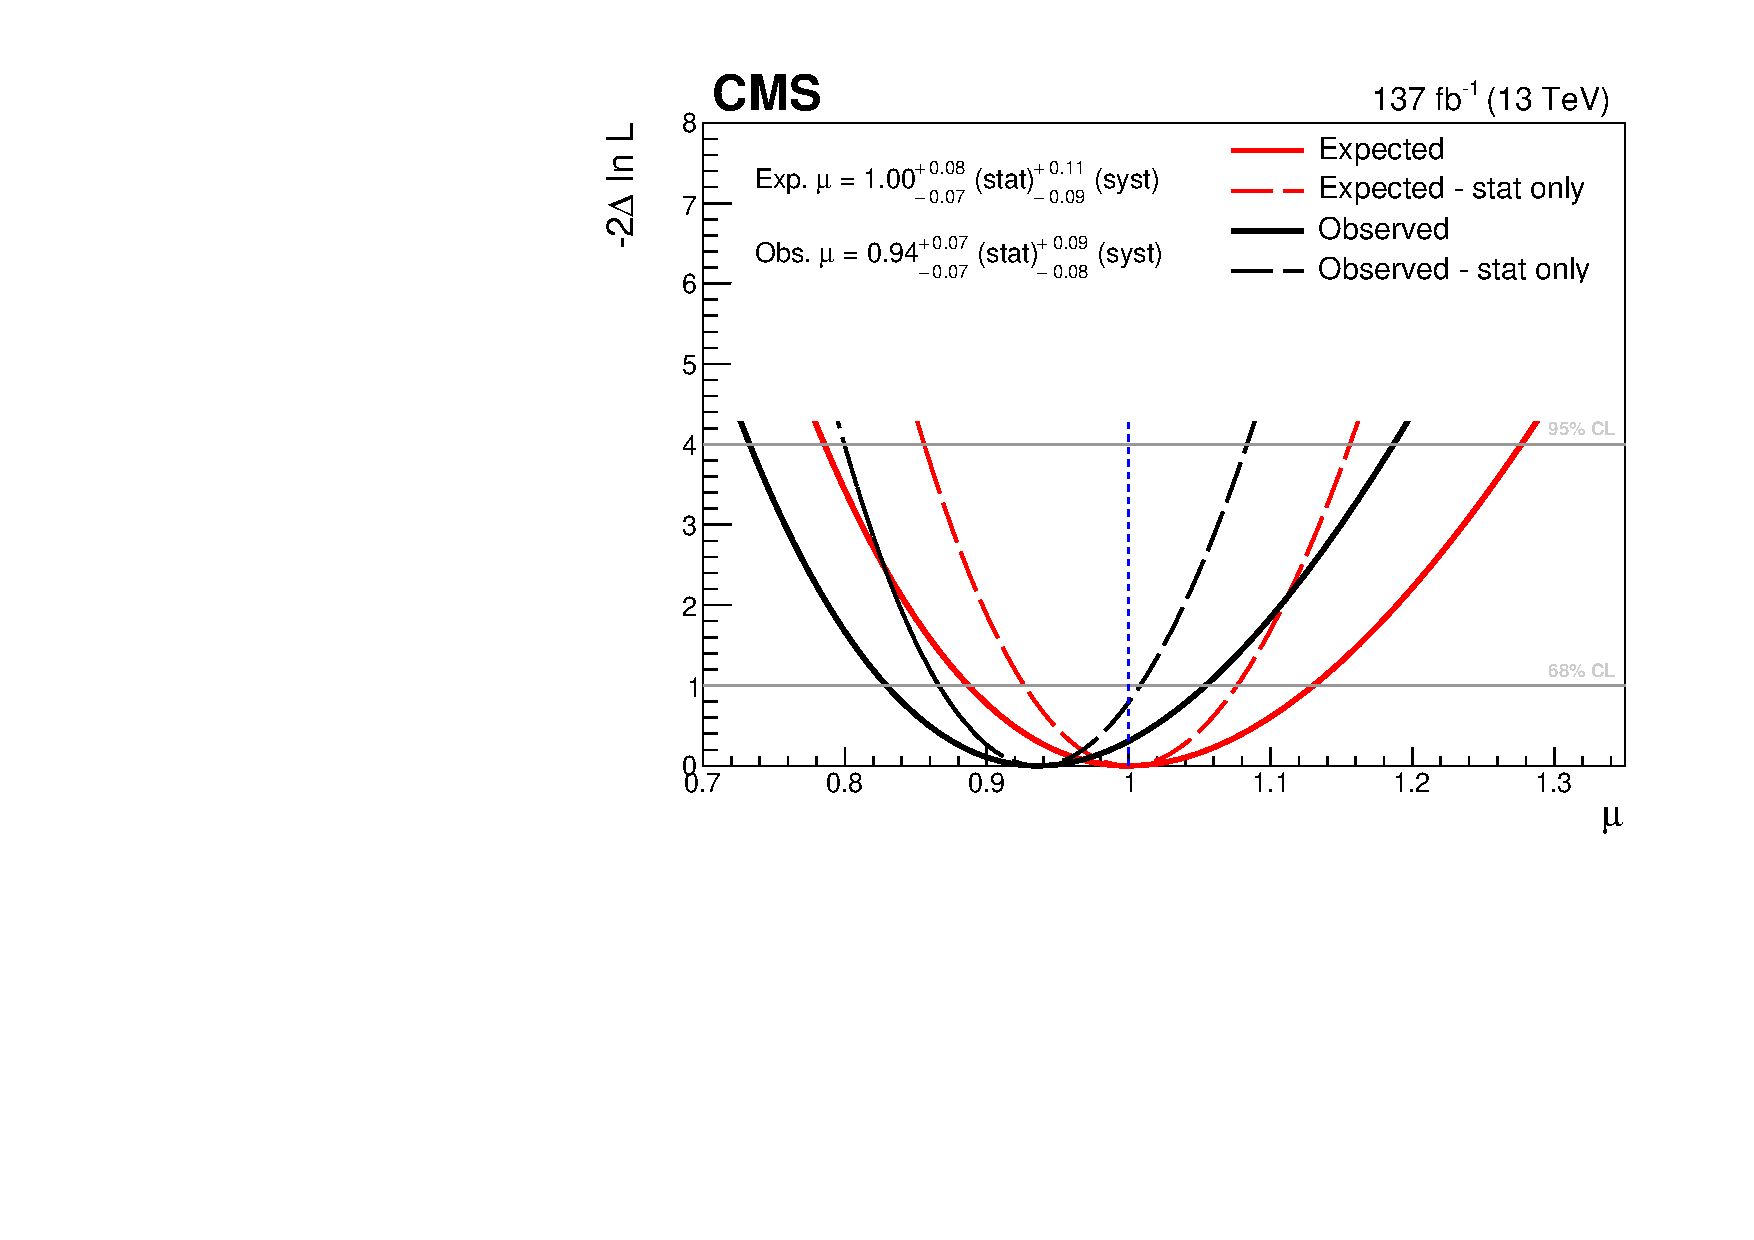
\includegraphics[width=0.49\linewidth]{Figures/results/signalstrength/InclusiveMu_125_38.pdf}
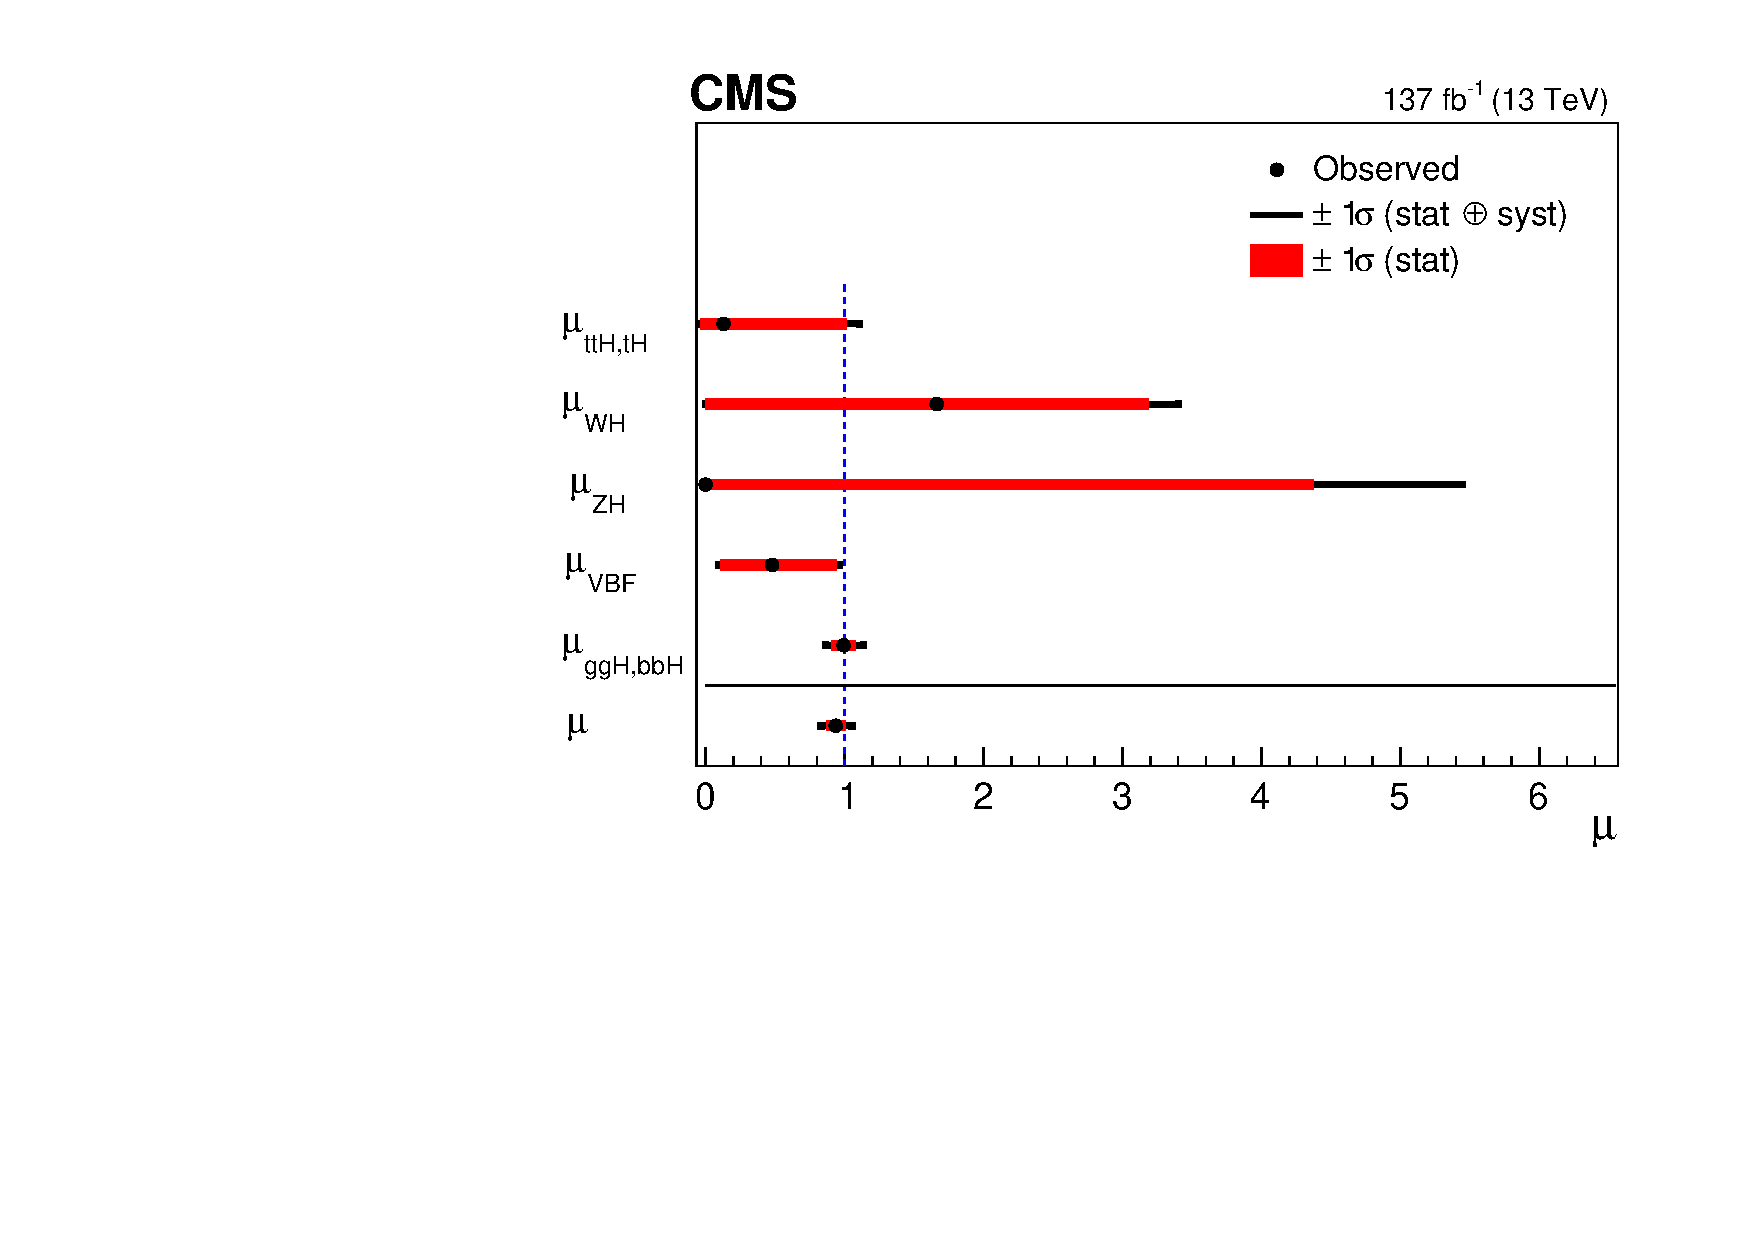
\includegraphics[width=0.49\linewidth]{Figures/results/signalstrength/mu_stage0_125_38.pdf}
\caption{
(Left) The observed and expected profile likelihood scans of the inclusive signal-strength modifier. The scans are shown both with (solid line) and without (dashed line) systematic uncertainties.
(Right) Results of likelihood scans for the signal-strength modifiers corresponding to the five main SM Higgs boson production mechanisms, compared to the inclusive signal strength modifier  $\mu$ shown as a vertical line.
The thick black lines report the $1\sigma$ confidence intervals including both statistical and systematic sources.
The thick red lines report the statistical uncertainties of the $1\sigma$ confidence intervals.
\label{fig:mucat}}
\end{center}
\end{figure}
%%%%%%%%%%%%%%%%%%%%%%%

\begin{table}[hb]
	\begin{center}
		\caption{
		Best-fit values and $\pm 1\sigma$ uncertainties for the expected and observed signal-strength modifiers.
		The uncertainty numbers are broken into statistical and systematic sources.
		The expected results are obtained for $\mH=125.38~\mathrm{GeV}$. %the observed results are obtained with $\mH$ profiled in the fit.
		\label{tab:sigstr}
			}
    \renewcommand{\arraystretch}{1.5}
    \begin{tabular}{ccc}
	\hline
	& Expected & Observed \\
	\hline
	$\mu_{\Pg\Pg\PH,\bbH}$ & $1.00~^{+0.10}_{-0.10}$~(stat)$~^ {+0.12}_{-0.10}~$(syst) & $0.99 ^{+0.09 }_{-0.09}$(stat)~$~^ {+0.11}_{-0.09}~$(syst) \\
  $\mu_{\mathrm{VBF}}$ & $1.00~^{+0.53}_{-0.44}$~(stat)$~^ {+0.18}_{-0.12}~$(syst) & $0.48 ^{+0.46}_{-0.37}$(stat)~$~^ {+0.14}_{-0.10}~$(syst) \\
  $\mu_{\ZH}$ & $1.00~^{+4.79}_{-1.00}~$(stat)$~^ {+6.76}_{-0.00}~$(syst) & $0. ^{+4.38}_{-0.00}$(stat)~$~^ {+3.24}_{-0.00}~$(syst) \\
  $\mu_{\WH}$ & $1.00~^{+1.83}_{-1.00}~$(stat)$~^{+0.75}_{-0.00}~$(syst) & $1.66 ^{+1.52}_{-1.66}$(stat)~$~^ {+0.85}_{-0.00}~$(syst) \\
	$\mu_{\ttH,\tH}$ & $1.00~^{+1.23}_{-0.77}~$(stat)$~^ {+0.51}_{-0.06}~$(syst) & $0.17 ^{+0.88}_{-0.17}$(stat)~$~^{+0.42}_{-0.00}~$(syst) \\
		  	\hline
	$\mu$ & $1.00~^{+0.08}_{-0.07}$~(stat)~$^{+0.10}_{-0.08}$~(syst) & $0.94~^{+0.07}_{-0.07}$~(stat)~$^{+0.09}_{-0.08}$~(syst)\\
	\hline
\end{tabular}
	\end{center}
\end{table}

Two signal strength modifiers $\muF$ and $\muV$ are introduced as scale factors for the fermion- and vector-boson induced contribution to the expected SM cross section.
A two-parameter fit is performed simultaneously to all reconstructed event categories, leading to the measurements of $\muF=\valMuF$ and $\muV=\valMuV$. 
%profiling $\mH$, 
The expected meaurements obtained for $\mH=125.38~\mathrm{GeV}$ are $\muF~=~1.00~^{+0.15}_{-0.13}$ and $\muV~=~1.00~^{+0.39}_{-0.33}$.
The 68\% and 95\%~CL contours in the ($\muF,\muV$) plane are shown in Fig.~\ref{fig:mu2D} and the SM predictions lie within the 68\%~CL regions of this measurement.

% %%%%%%%%%%%%%%%%%%%%%%%
\begin{figure}[!htb]
\begin{center}
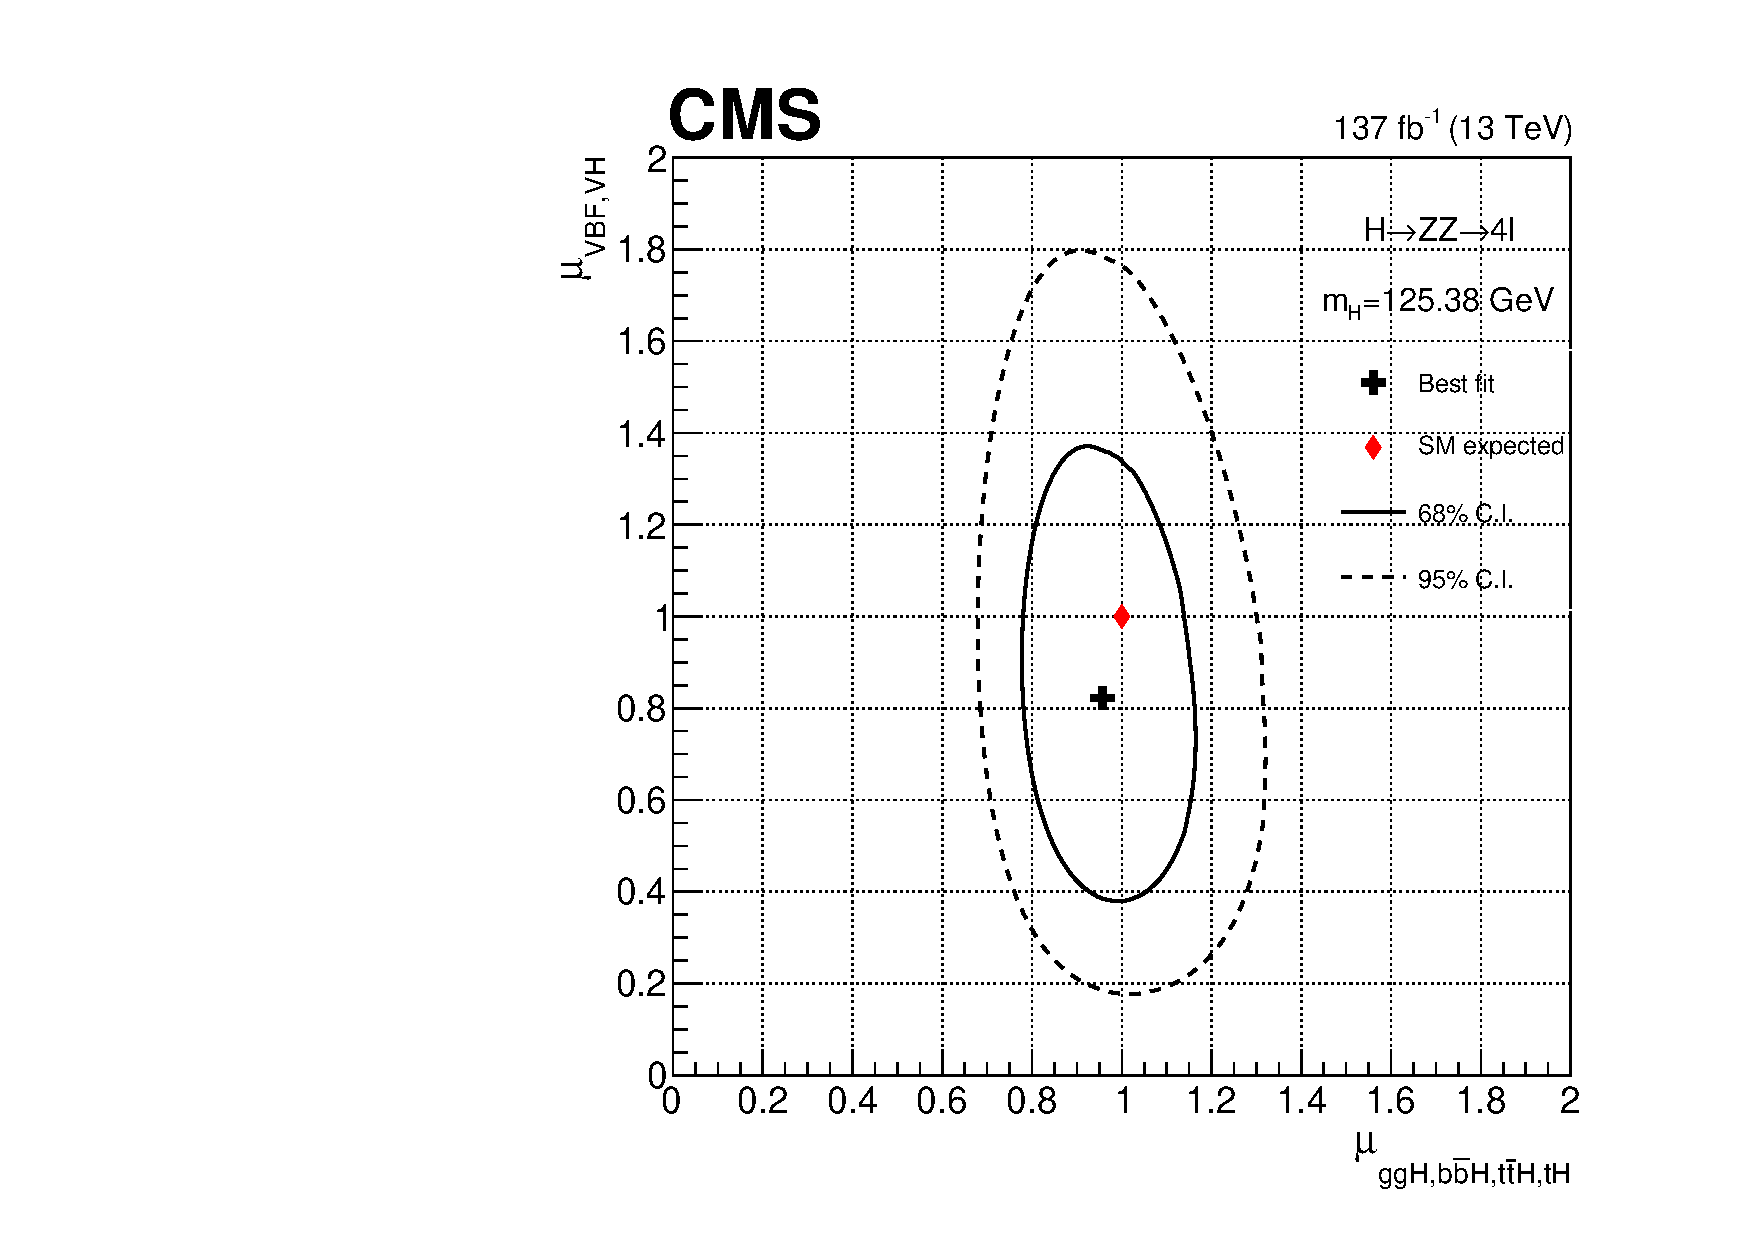
\includegraphics[width=0.9\linewidth]{Figures/results/signalstrength/rvrf_125_38.pdf}
\caption{
Result of the 2D likelihood scan for the $\muF$ and $\muV$ signal-strength modifiers.
The solid and dashed contours show the 68\% and 95\% CL regions, respectively.
The cross indicates the best-fit value, and the diamond represents the expected value for the SM Higgs boson.
\label{fig:mu2D}}
\end{center}
\end{figure}
% %%%%%%%%%%%%%%%%%%%%%%%






% OLD text

%\textbf{FIXME: Results shown here used 2017 yield parameterization and categorization but systematics, templates, etc... from 2016 analysis}
%With a 2D fit, the signal strength is measured to be $\mu = 0.98^{+0.11}_{-0.10}$  for a fixed mass hypothesis of $\mH=125~\GeV$. %.09~\GeV$
% (and $X.XX^{+X.XX}_{-X.XX}$ when constraining the Higgs boson mass to $\mH = 125.09\pm0.24\GeV$) 
 %for the inclusive event sample. The results are compared to the expected signal-strength modifiers in Table~\ref{tab:sigstr}.

%{\renewcommand{\arraystretch}{1.2}
%\begin{table}[!hb]
%\begin{center}
%\caption{ Expected and observed signal-strength modifiers. \textbf{FIXME: Numbers to be split by syst/stat uncertainties}
%\label{tab:sigstr}}
%\begin{tabular}{l|c|ccccc}
%   &  Inclusive & $\mu_{\Pg\Pg\PH}$ & $\mu_{\mathrm{VBF}}$ &  $\mu_{\rm VHhad}$ & $\mu_{\rm VHlep}$ & $\mu_{\ttH}$ \\
%\hline
%Expected  & $1.00^{+0.15}_{-0.14}({\rm stat.})^{+0.10}_{-0.09}({\rm sys.})$ & $1.00^{+0.24}_{-0.21}$ & $1.00^{+0.25}_{-0.97}$ & $1.00^{+3.97}_{-1.00}$  & $1.00^{+3.93}_{-1.00}$ & $1.00^{+3.22}_{-1.00}$ \\
%Expected &  $1.00^{+0.17}_{-0.15}$ & $1.00^{+0.21}_{-0.19}$ & $1.00^{+1.11}_{-0.85}$ & $1.00^{+3.84}_{-1.00}$  & $1.00^{+2.86}_{-1.00}$ & $1.00^{+2.50}_{-1.00}$ \\
%Observed  & $XX^{+XX}_{-XX}({\rm stat.})^{+XX}_{XX}({\rm sys.})$ & $XX^{XX}_{XX}$ & $XX^{XX}_{XX}$  & $XX^{+XX}_{-XX}$ & $0.00^{+XX}_{-XX}$ &  $0.00^{+XX}_{-XX}$ \\
%\hline
%\end{tabular}
%\end{center}
%\end{table}
%}

%{\renewcommand{\arraystretch}{1.2}
%\begin{table}[!hb]
%\begin{center}
%\caption{ Expected and observed signal-strength modifiers with 2D scan (with kinematic discriminant).
%\label{tab:sigstr}}
%\resizebox{\textwidth}{!}{\begin{tabular}{l|c|ccccc}
%   &  Inclusive & $\mu_{\Pg\Pg\PH}$ & $\mu_{\mathrm{VBF}}$ &  $\mu_{\rm VH}$ & $\mu_{\ttH}$\\
%\hline
%Expected  & $1.00^{+0.12}_{-0.10}$ & $1.00^{+0.14}_{-0.12}$ & $1.00^{+0.60}_{-0.47}$  & ${1.00}^{+1.09}_{-0.82}$ & $1.00^{+1.17}_{-0.72}$ \\
%Observed  & $0.97^{+0.11}_{-0.10}$ & ${0.67}^{+0.51}_{-0.39}$ & ${0.67}^{+0.51}_{-0.39}$  & ${1.21}^{+1.08}_{-0.85}$ & ${0.33}^{+0.91}_{-0.33}$\\

%\hline
%\end{tabular}}
%\end{center}
%\end{table}
%}


%\begin{figure}[htb]
%\begin{center}
%\includegraphics[width=0.6\linewidth]{Figures/Results/signalstrength/signal_strength_categories_unblind_2017.pdf}
%\caption{Values of $\mu=\sigma/\sigma_{SM}$ for the six categories. 
%The vertical line shows the combined $\mu$, together with its associated $\pm$ 1$\sigma$ uncertainties shown as filled band.  
%The horizontal bars indicate the $\pm$ 1$\sigma$ uncertainties on $\mu$ for the different categories. 
%The uncertainties include both statistical and systematic sources.
%\label{fig:mucat}}
%\end{center}
%\end{figure}

% TO BE ADDED. COMMENTED FOR NOW
%Two signal-strength modifiers $\muF$ and $\muV$ are introduced as scale factors for the fermion and vector-boson induced contribution to the expected SM cross section.
%A two-dimensional fit is performed, profiling the likelihood for all nuisance parameters including the \mH, leading to the measurements of  $\muF=0.98^{+0.13}_{-0.12}$ and $\muV=0.85^{+0.37}_{-0.30}$.
%The 68\% and 95\% CL contours in the ($\muF,\muV$) plane are shown in Fig.~\ref{fig:RVRF}. 
%When constraining the Higgs boson mass to $\mH = 125.09\pm0.24\GeV$ instead of fixing it, the best fit values are $\muF=X.XX$ and $\muV=X.XX$.
%All results for $\mu$, $\muF$ and $\muV$ are reported in Tables~\ref{tab:muvalues_exp} and~\ref{tab:muvalues_obs}.

%\begin{figure}[htb]
%\begin{center}
%    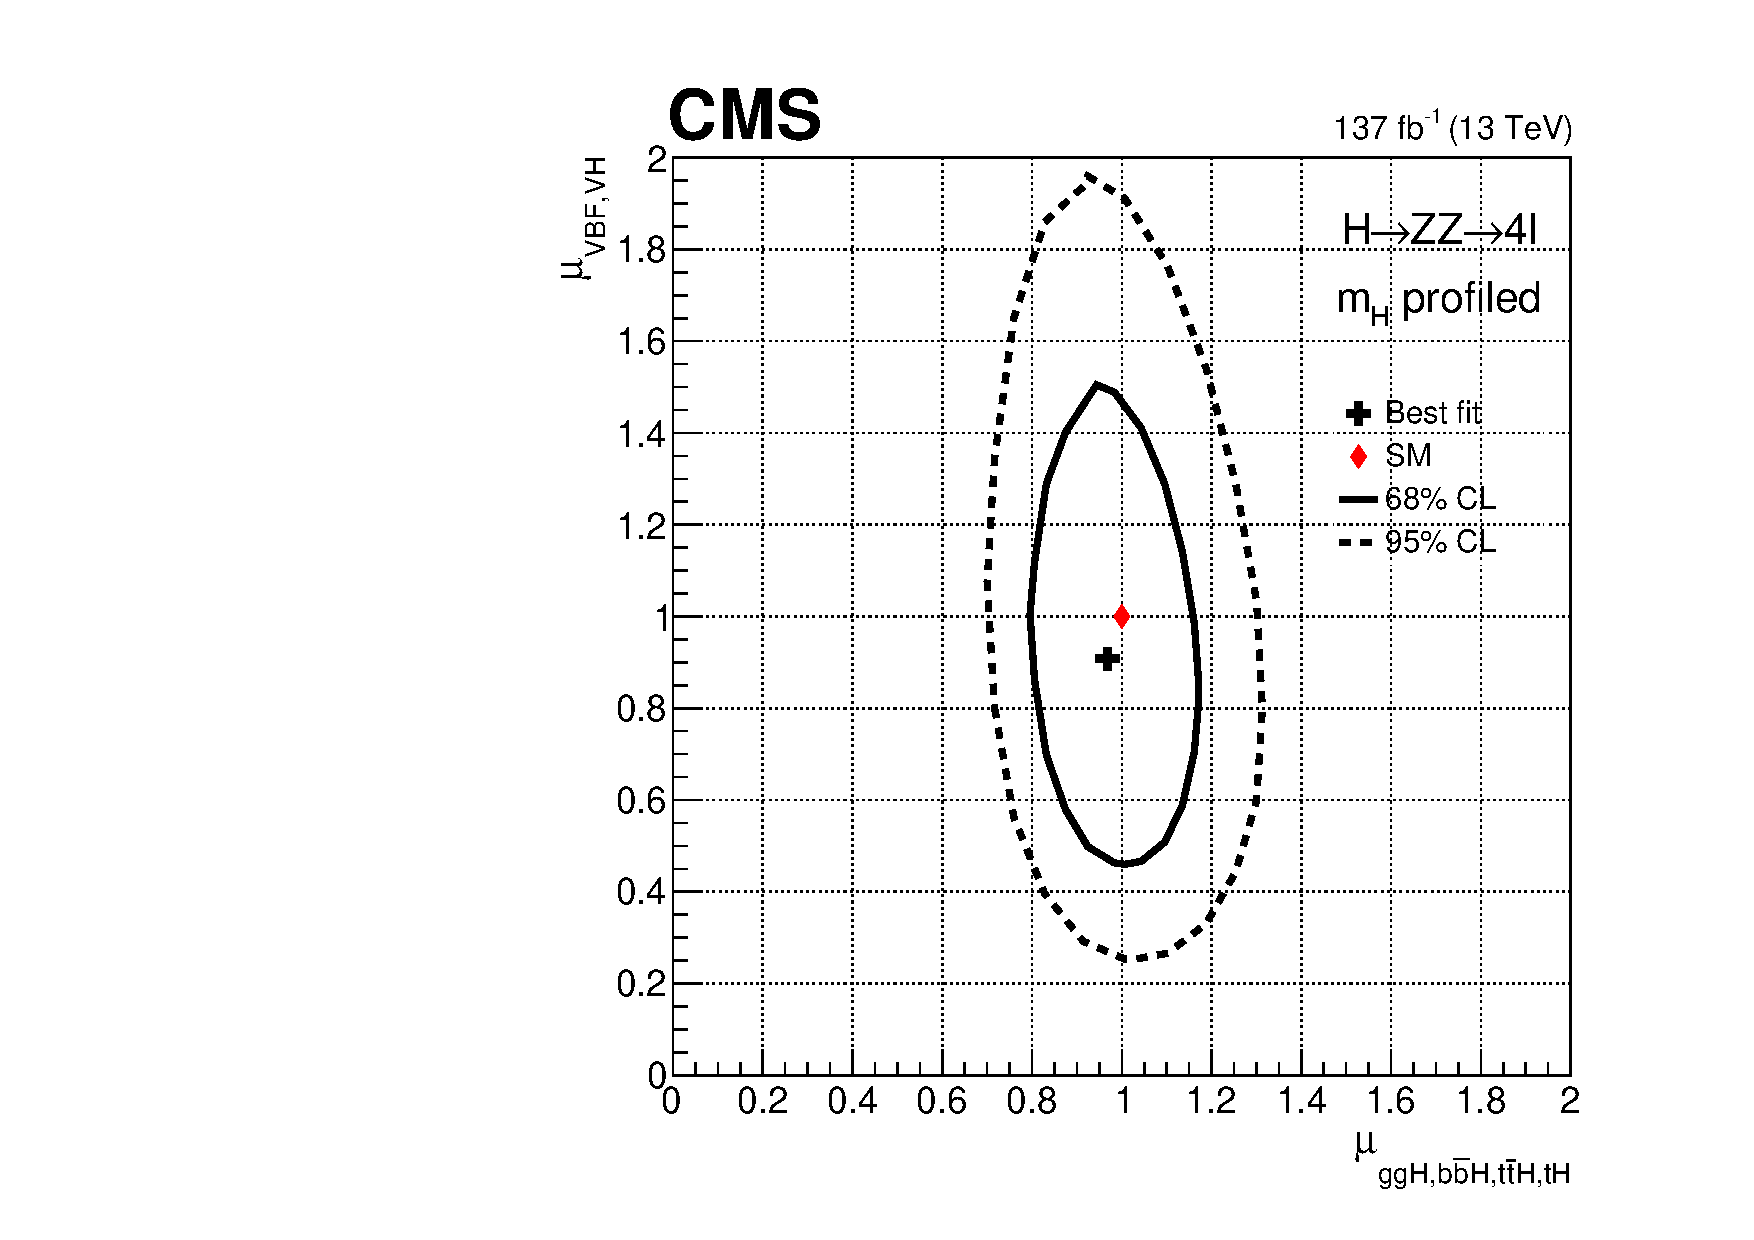
\includegraphics[width=0.6\linewidth]{Figures/results/signalstrength/rvrf.pdf}
%    \caption{ Result of the 2D likelihood scan for the $\muF$ and $\muV$ signal-strength modifiers. 
%   The solid and dashed contours show the 68\% and 95\% CL regions, respectively. 
%    The cross indicates the best-fit values, and the diamond represents the expected values for the SM Higgs boson.
%\label{fig:RVRF}}
%\end{center}
%\end{figure}


%{\renewcommand{\arraystretch}{1.5}
%%%============
%\begin{table}[!hb]
%\begin{center}
%\caption{Expected signal strength values for different measurement setups.
%\label{tab:muvalues_exp}}
%\begin{tabular}{lcccc}
%\hline  
% Categorization  & 1D: ${\cal L}(m_{4l})$ & 2D: ${\cal L}(m_{4l},\KD)$ &   1D: ${\cal L}(m_{4l}')$ & 2D: ${\cal L}(m_{4l}',\KD)$ \\ \hline 
%Inclusive &  $\mu=$1.000$^{+XX}_{-XX}$ & $\mu=$1.000$^{+XX}_{-XX}$ &  $\mu=$1.000$^{+XX}_{-XX}$ & $\mu=$1.000$^{+XX}_{-XX}$ \\ \hline
% &  $\mu=$1.000$^{+XX}_{-XX}$ & $\mu=$1.000$^{+XX}_{-XX}$ &  $\mu=$1.000$^{+XX}_{-XX}$ & $\mu=$1.000$^{+XX}_{-XX}$ \\
%Two categories & $\muV$=1.000$^{+XX}_{-XX}$ & $\muV=$1.000$^{+XX}_{-XX}$ &  $\muV=$1.000$^{+XX}_{-XX}$ & $\muV=$1.000$^{+XX}_{-XX}$ \\
% & $\muF=$1.000$^{+XX}_{-XX}$ & $\muF=$1.000$^{+XX}_{-XX}$ &  $\muF=$1.000$^{+XX}_{-XX}$ & $\muF=$1.000$^{+XX}_{-XX}$ \\
%\hline
%\end{tabular}
%\end{center}
%\end{table}
%%%============
%}
%
%{\renewcommand{\arraystretch}{1.5}
%%%============
%\begin{table}[!hb]
%\begin{center}
%\caption{Expected and observed signal strength values for different measurement setups.
%\label{tab:muvalues_obs}}
%\begin{tabular}{lcccc}
%\hline  
% Categorization  & 1D: ${\cal L}(m_{4l})$ & 2D: ${\cal L}(m_{4l},\KD)$ &   1D: ${\cal L}(m_{4l}')$ & 2D: ${\cal L}(m_{4l}',\KD)$ \\ \hline 
%Inclusive &  $\mu=$X.XX$^{+XX}_{-XX}$ & $\mu=$X.XX$^{+XX}_{-XX}$ &  $\mu=$X.XX$^{+XX}_{-0.XX}$ & $\mu=$X.XX$^{+XX}_{-XX}$ \\ \hline
% &  $\mu=$X.XX$^{+XX}_{-XX}$ & $\mu=$X.XX$^{+XX}_{-XX}$ &  $\mu=$X.XX$^{+XX}_{-XX}$ & $\mu=$X.XX$^{+XX}_{-XX}$ \\
%Two categories & $\muV$=X.XX$^{+XX}_{-XX}$ & $\muV=$X.XX$^{+XX}_{-XX}$ &  $\muV=$X.XX$^{+XX}_{-XX}$ & $\muV=$X.XX$^{+XX}_{-XX}$ \\
% & $\muF=$X.XX$^{+XX}_{-XX}$ & $\muF=$X.XX$^{+XX}_{-XX}$ &  $\muF=$X.XX$^{+XX}_{-XX}$ & $\muF=$X.XX$^{+XX}_{-XX}$ \\
%\hline
%\end{tabular}
%\end{center}
%\end{table}
%%%============
%}

%Signal-strength modifiers for the five main Higgs production modes, $\mu_{\Pg\Pg\PH}$, $\mu_{\mathrm{VBF}}$, $\mu_{\WH}$, $\mu_{\ZH}$ and $\mu_{\ttH}$ are also introduced as scale factors to the expected SM cross section. 
%Similarly, the fits are performed fixing the mass to $\mH = 125~\GeV$ and profiling the likelihood for all nuisance parameters, leading to the results 
%reported in Table~\ref{tab:muprocesses} and 
%illustrated in Fig.~\ref{fig:muprocesses},
% Three models are tested, 
% in Fig.~\ref{fig:muprocesses}(top left) $\mu_{\WH}$ are $\mu_{\ZH}$ are separated, 
% in Fig.~\ref{fig:muprocesses}(top right) $\mu_{\WH}$ are $\mu_{\ZH}$ are grouped in $\mu_{\VH}$, 
% and in Fig.~\ref{fig:muprocesses}(bottom) 
%where $\mu_{\WH}$ and  $\mu_{\ZH}$ are merged to $\mu_{VH}$.
%splitted in the leptonically decay bosons  $\mu_{\WH lep}$/$\mu_{\ZH lep}$ and hadronically decay  bosons $\mu_{\WH lep}$/$\mu_{\ZH lep}$.


%%%============
%\begin{table}[hb]
%\begin{center}
%\caption{Expected and observed results of likelihood scans for the signal strength modifiers corresponding to the five main Higgs boson production modes.
%\label{tab:muprocesses}}
%\begin{tabular}{l|c|c}
%\hline
%   & Expected & Observed  \\
%\hline
%$\mu_{\Pg\Pg\PH}$  & 1.00$^{+0.48}_{-0.43}$ & 1.09$^{+0.47}_{-0.42}$  \\
%$\mu_{\mathrm{VBF}}$  & 1.00$^{+2.51}_{-1.00}$ & 0.00$^{+0.59}_{-0.00}$  \\
%$\mu_{\WH}$  & 1.00$^{+9.20}_{-1.00}$ & 0.00$^{+8.49}_{0.00}$  \\
%$\mu_{\ZH}$  & 1.00$^{+17.96}_{-1.00}$ & 2.48$^{+17.43}_{-2.48}$  \\
%$\mu_{\ttH}$  & 1.00$^{+8.01}_{-1.00}$ & 8.83$^{+16.39}_{-8.83}$ \\
%\hline
%\end{tabular}
%\end{center}
%\end{table}
%%%============

%\begin{figure}[htb]
%\begin{center}
% \includegraphics[width=0.45\linewidth]{Figures/Results/signalstrength/compatibility_process_ZHWH.pdf}
% \includegraphics[width=0.45\linewidth]{Figures/Results/signalstrength/compatibility_process_VH.pdf} \\
%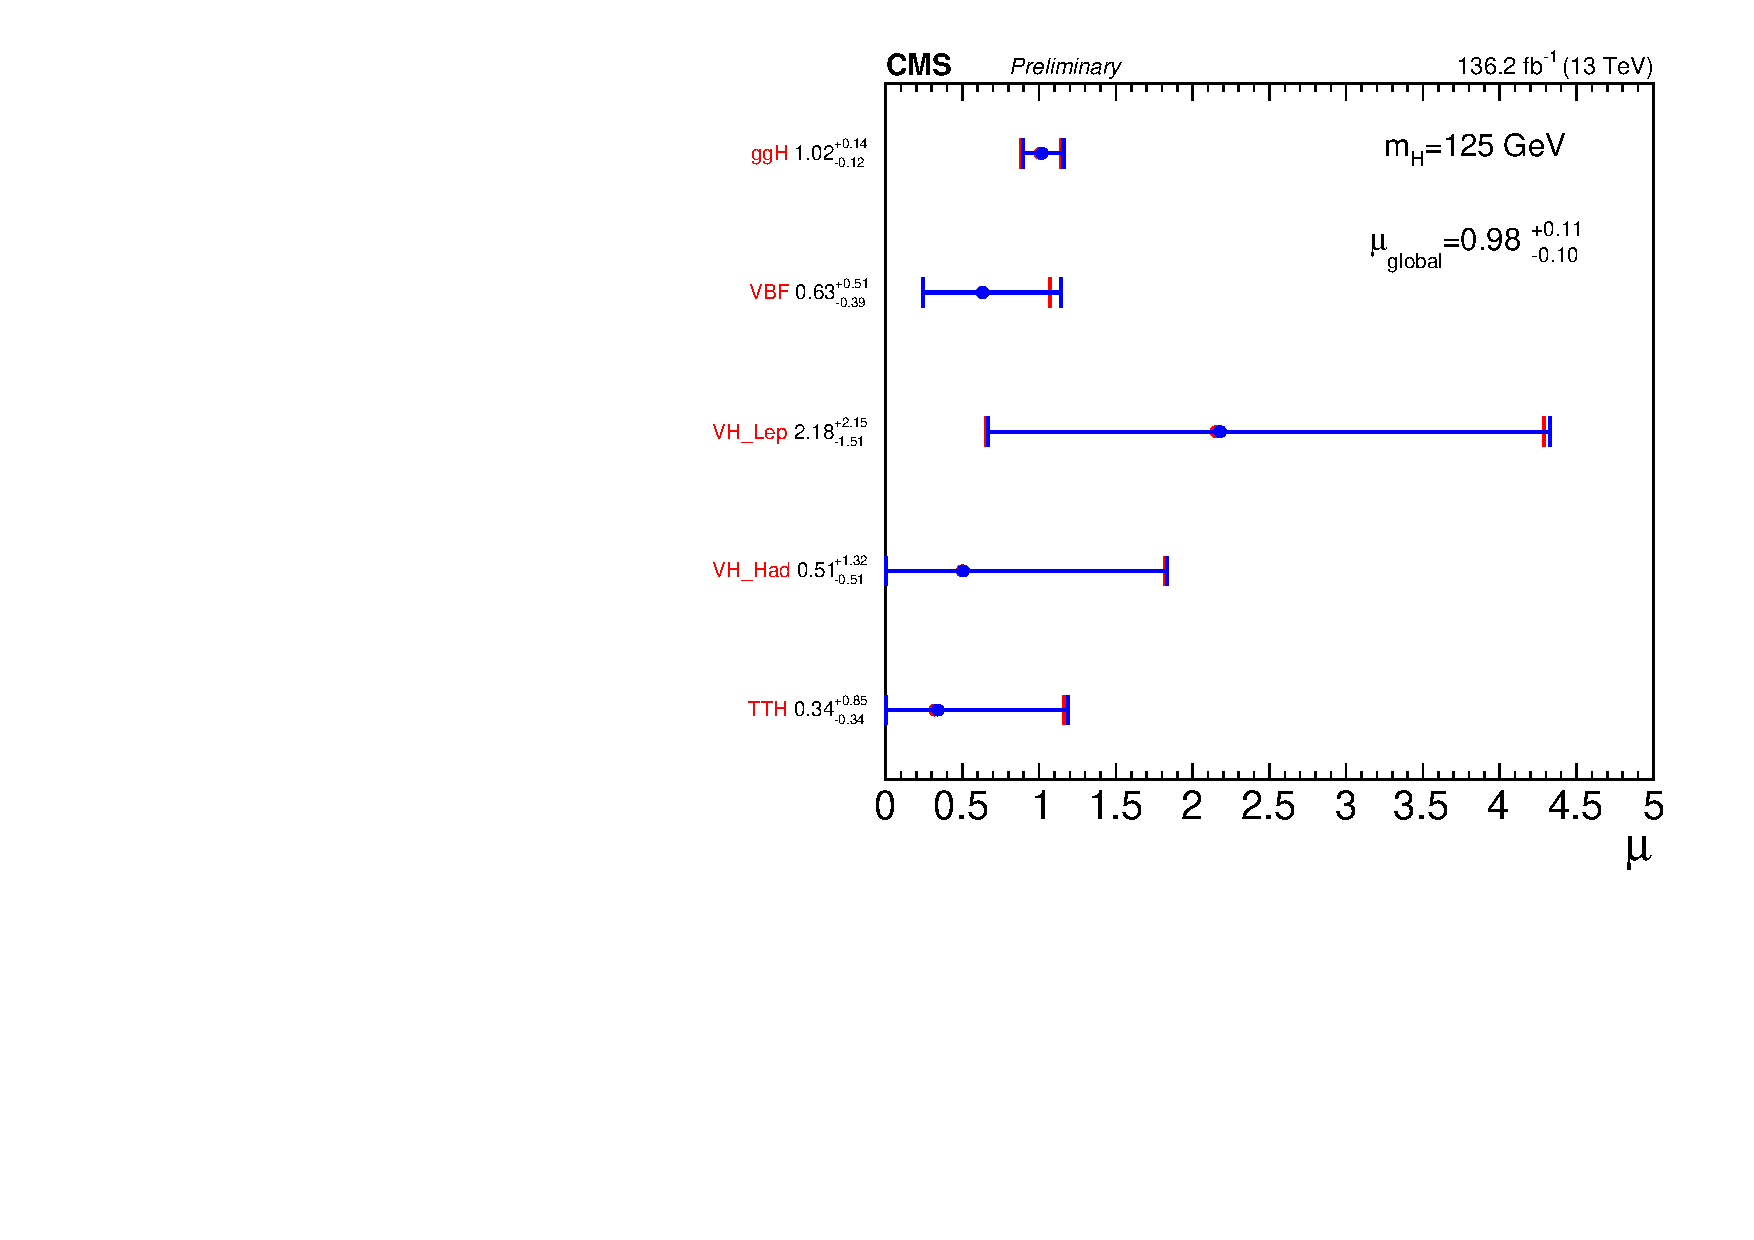
\includegraphics[width=0.80\linewidth]{Figures/results/signalstrength/mu_stage0_hadlep1_obs.pdf}
%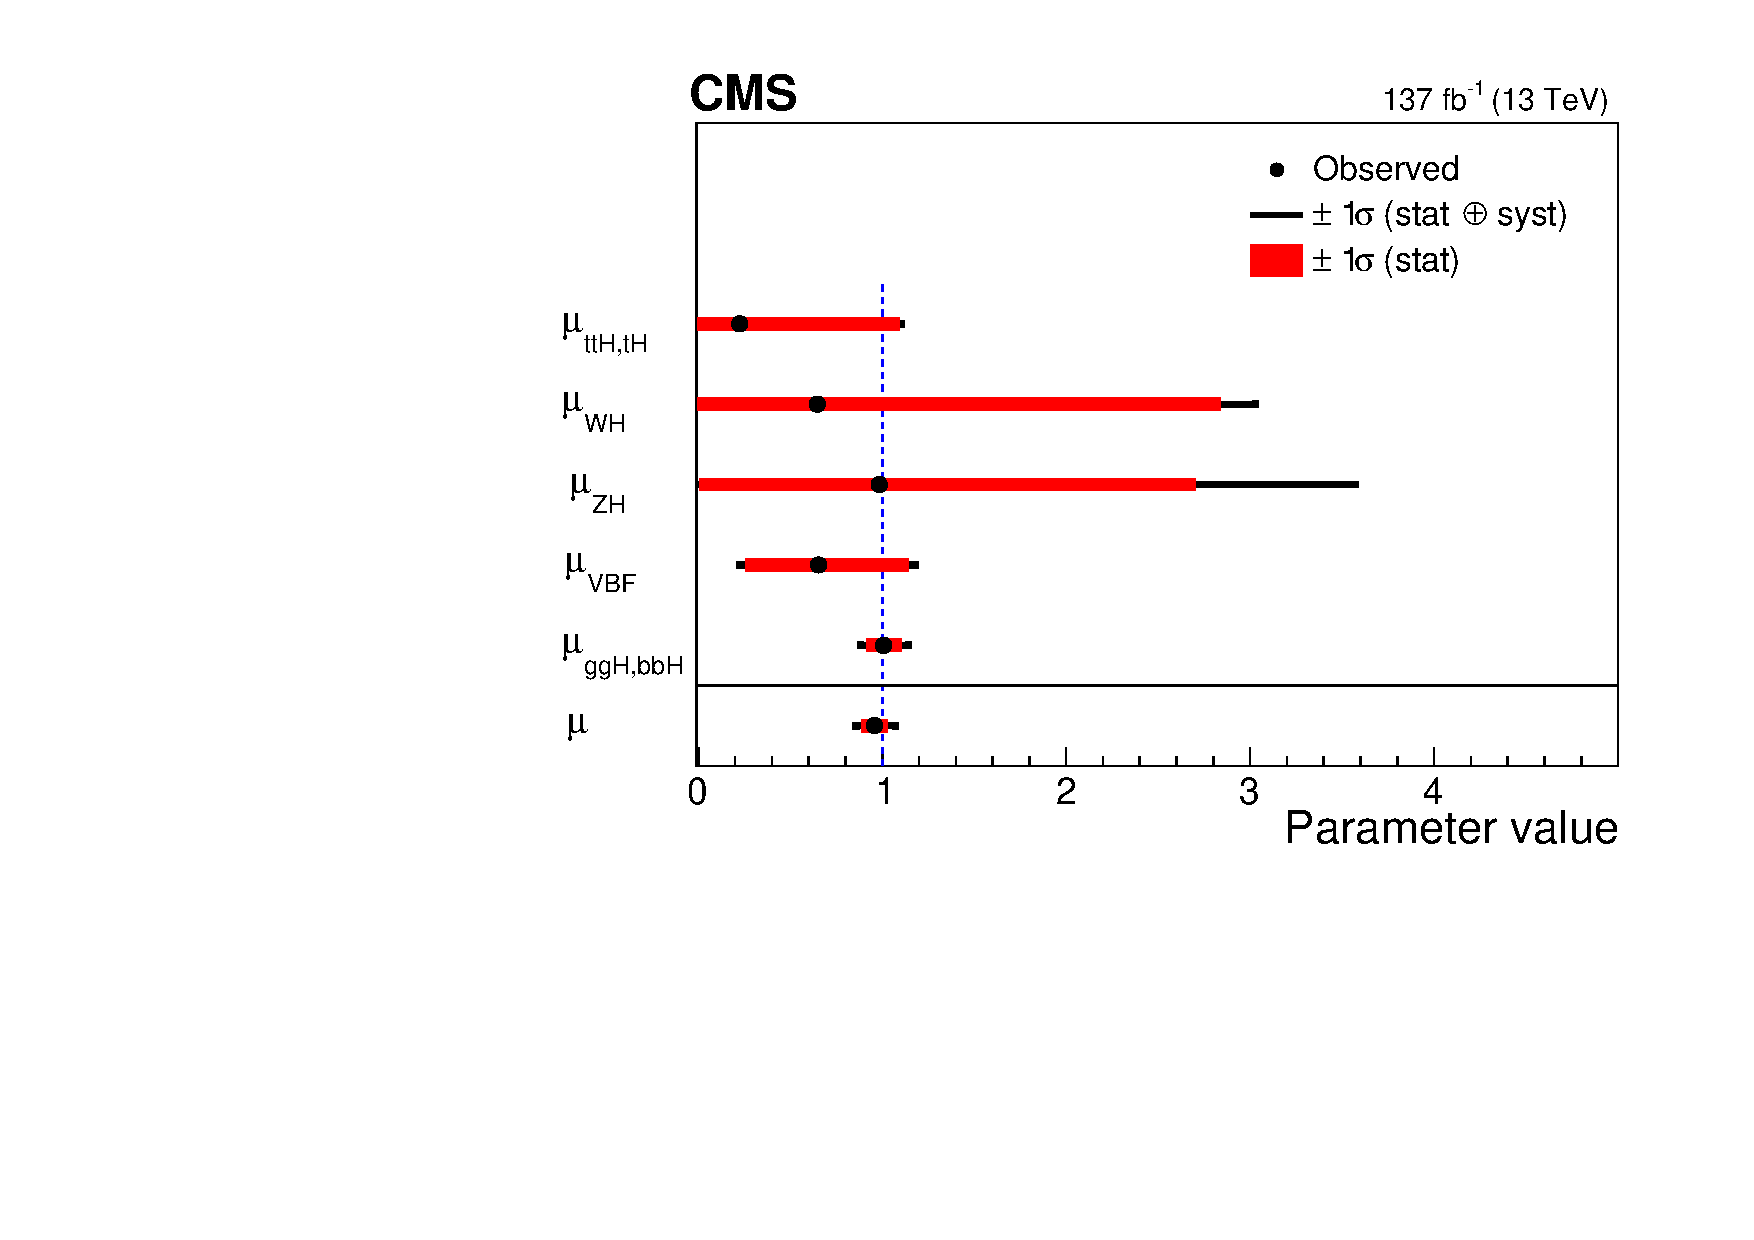
\includegraphics[width=0.45\linewidth]{Figures/results/signalstrength/mu_stage0.pdf}
%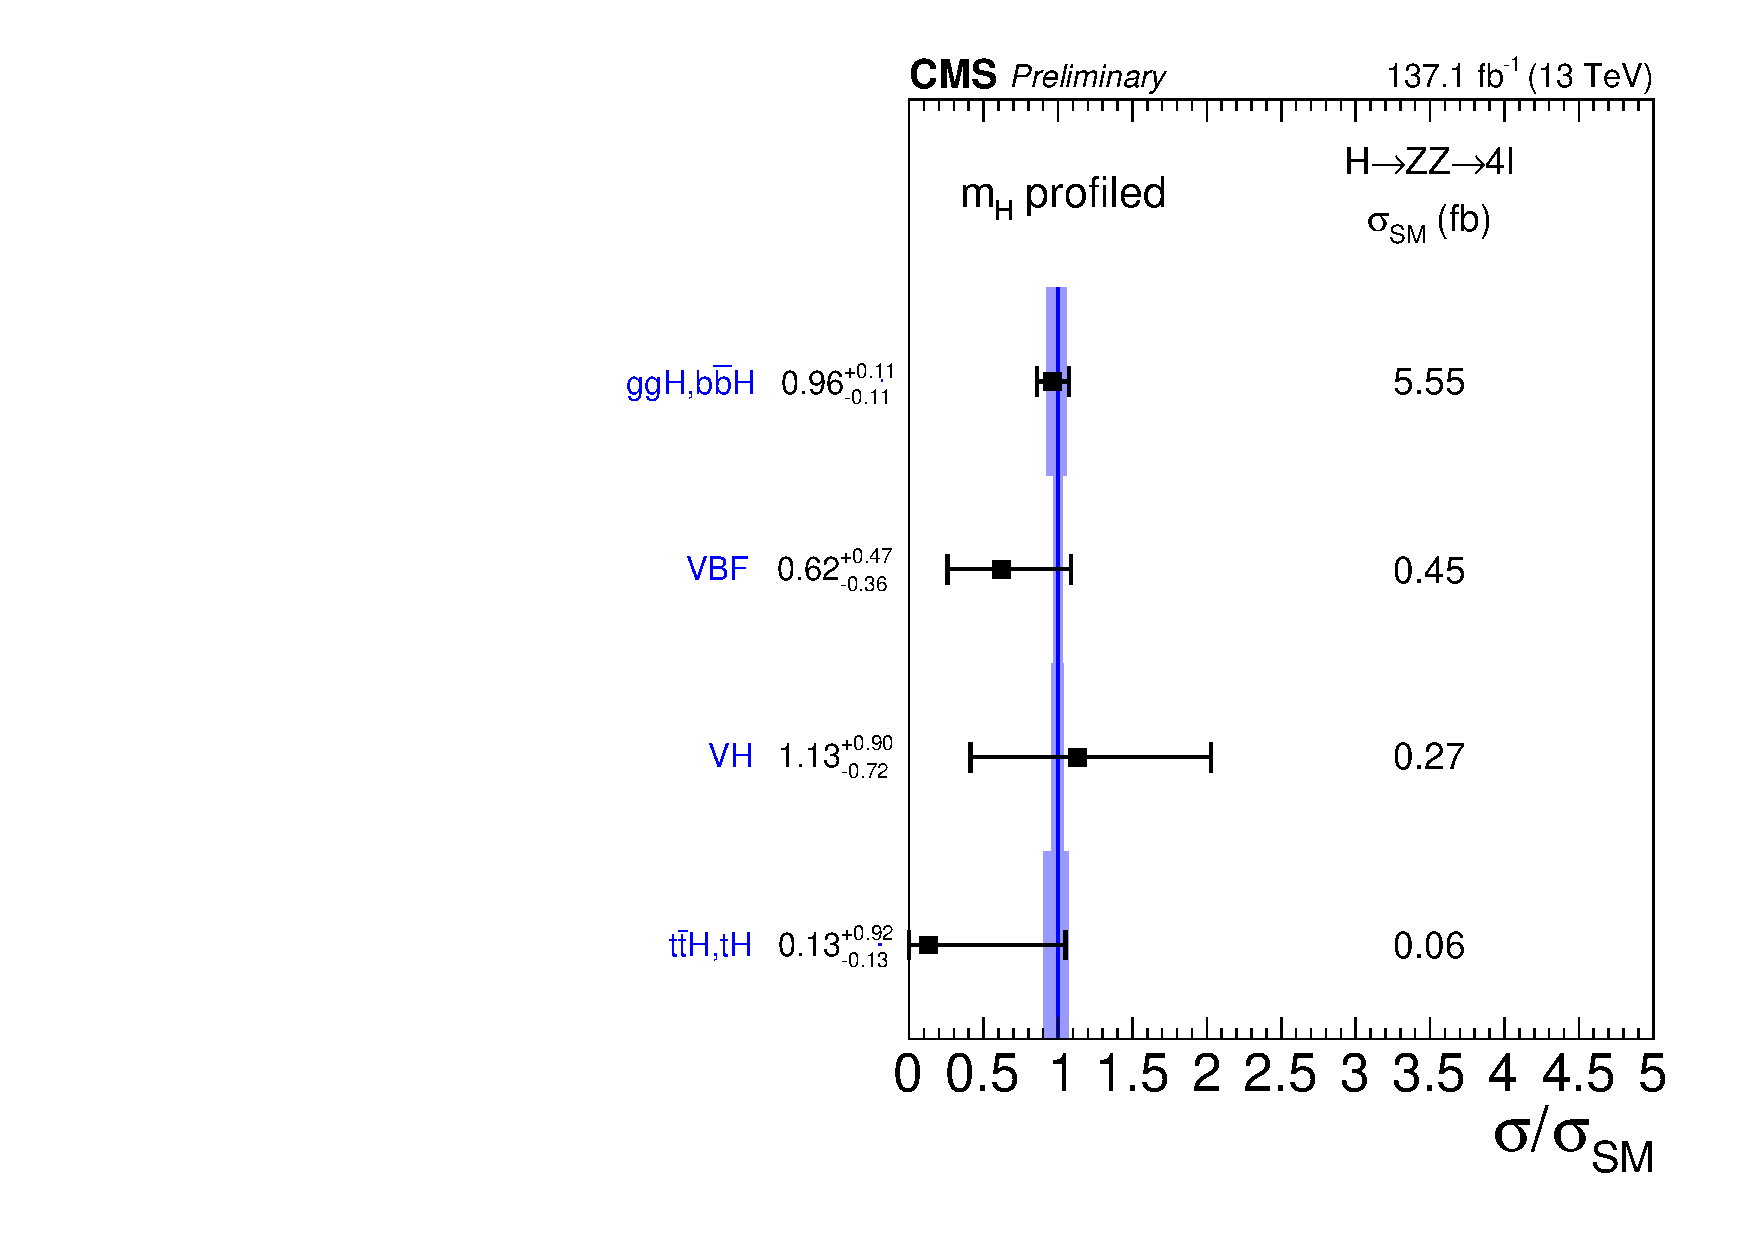
\includegraphics[width=0.45\linewidth]{Figures/results/signalstrength/mu_stage0_xsec.pdf}
%\caption{Results of likelihood scans for the signal strength modifiers (left) and cross section (right) corresponding to the four main Higgs boson production modes.
%On the left figure, the vertical line shows the combined $\mu$, together with its associated $\pm$ 1$\sigma$ uncertainties shown as filled band.  
%On the right figure, the band of the vertical line shows the theoretical uncertainties on the SM cross sections.
%The horizontal bars indicate the $\pm$ 1$\sigma$ uncertainties on $\mu$ for the different production modes. 
%The uncertainties include both statistical and systematic sources.
%\label{fig:muprocesses}}
%\end{center}
%\end{figure}
 
%
%\clearpage 
%
%%\subsection{Simplified Template Cross Sections}
%%\label{sec:stxs}
%\subsection{Simplified template cross section}
\label{subsec:stxs}

The measurements of the product $\sigma\cdot\mathcal{B}$ of the Higgs boson production cross-section and the branching ratio normalised by the SM expectation,
$(\sigma\cdot\mathcal{B})_{\mathrm{SM}}$, for the stages of production bins defined in Section~\ref{subsec:STXS_Categories} are shown in Fig.~\ref{fig:stxs_0} for the stage 0 and in Fig.~\ref{fig:stxs_1} for the reduce stage 1.2.
The corresponding numerical values are given in Table~\ref{tab:stage0} and Table~\ref{tab:stage1p2}.
In the ratio calculation, the uncertainties in the SM expectation are not taken into account while the theoretical uncertainties which can cause migration of events between the various categories are kept in this measurement.
The correlation matrices are shown in Fig.~\ref{fig:corrmatrix}.
The dominant experimental sources of systematic uncertainty are the same as in the measurement of the signal-strength modifiers, while the dominant theoretical source is the uncertainty in the category migration for the $\ggH$ process.

As for the signal strenght, all measurements are reported at $\mH=125.38$ GeV.%, the best mass obtained by CMS from the combination of $H\rightarrow$ZZ and $H\rightarrow\gamma\gamma$ channels.

%%%%%%%%%%%%%%%%%%%%%%%
\begin{figure}[!htb]
\begin{center}
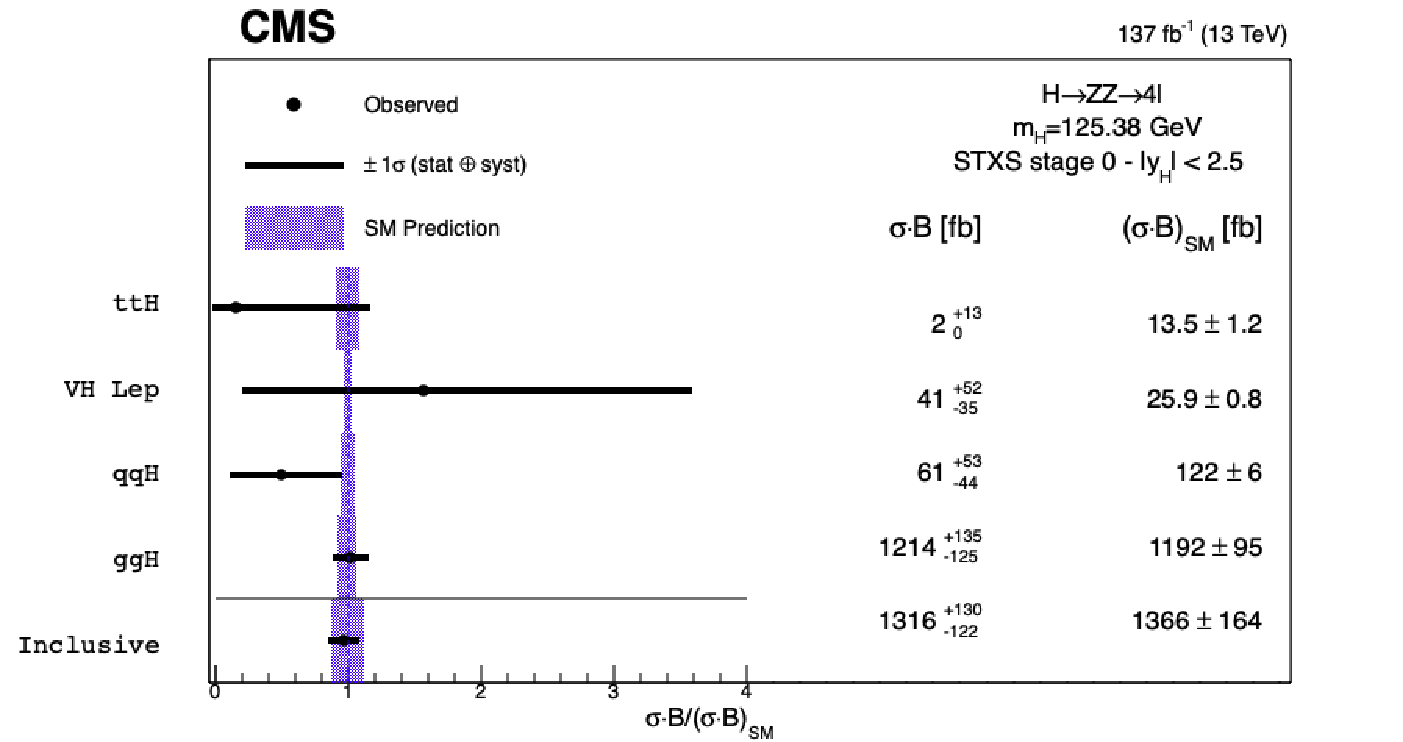
\includegraphics[width=0.7\linewidth]{Figures/results/stxs/stage0_125_38.pdf}
\caption{
		The ratios between measured cross sections $\sigma\cdot\mathcal{B}$ and the SM predictions $(\sigma\cdot\mathcal{B})_{\mathrm{SM}}$ for the stage 0 production bins.%, with $\mH$ profiled in the fit.
		The gray band around the vertical band shows the theoretical uncertainties on the SM Higgs boson cross section predictions for each of the bin.
		%Cross section values are reported for the best fit mass value $\mH = 125.1~\GeV$.
			\label{fig:stxs_0}
			}
	\end{center}
\end{figure}
%%%%%%%%%%%%%%%%%%%%%%%

%%%%%%%%%%%%%%%%%%%%%%%
\begin{table}[hb]
	\begin{center}
		\caption{
		Best-fit values and $\pm 1\sigma$ uncertainties for the measured cross sections $\sigma\cdot\mathcal{B}$ and the SM predictions $(\sigma\cdot\mathcal{B})_{\mathrm{SM}}$ for the stage 0 production bins.
		The results are obtained with $\mH=125.38$ GeV. % profiled in the fit.
		\label{tab:stage0}
			}
    \renewcommand{\arraystretch}{1.5}
    \begin{tabular}{ccc}
	\hline
	& $\sigma\cdot\mathcal{B}$ & $(\sigma\cdot\mathcal{B})_{\mathrm{SM}}$ \\
	\hline
        {\tt ttH} & $2~^{+13}_{-2}~$fb & $13~^{+18}_{-10}~$fb \\
	{\tt VH-lep} & $41~^{+52}_{-35}~$fb & $26~^{+42}_{-25}~$fb \\
	{\tt qqH} & $61~^{+53}_{-44}~$fb & $122~^{+62}_{-52}~$fb \\
%	{\tt ggH} & $1214~\pm 124~$fb & $1174\pm 123~$fb \\
	{\tt ggH} & $1214~^{+135}_{-125}~$fb & $1192~^{+139}_{-129}~$fb \\
    \hline
    {\tt Inclusive} & $1316~^{+130}_{-122}~$fb & $1366~^{+138}_{-126}~$fb  \\
	\hline
	\end{tabular}
 \end{center}
 \end{table}
 %%%%%%%%%%%%%%%%%%%%%%%

%%%%%%%%%%%%%%%%%%%%%%%
\begin{figure}[!htb]
\begin{center}
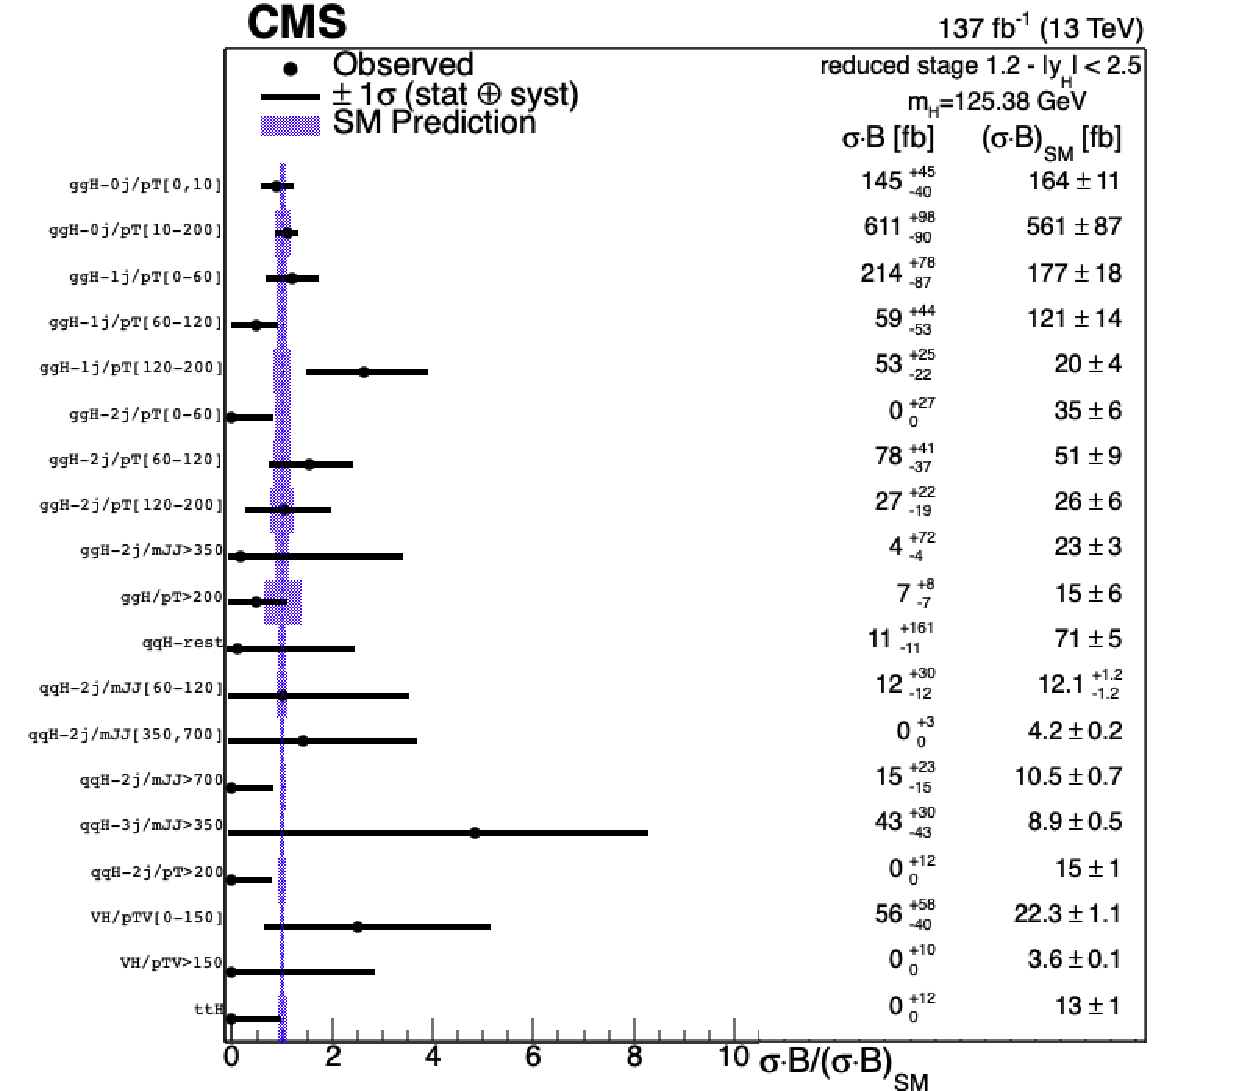
\includegraphics[width=0.9\linewidth]{Figures/results/stxs/stage1p2_125_38.pdf}
\caption{
The ratios between measured cross sections $\sigma\cdot\mathcal{B}$ and the SM predictions $(\sigma\cdot\mathcal{B})_{\mathrm{SM}}$ for the merged stage 1.2 production bins, with $\mH=125.38$ GeV. % profiled in the fit.
The gray band around the vertical band shows the theoretical uncertainties on the SM Higgs boson cross section predictions for each of the bin.
\label{fig:stxs_1}
}
\end{center}
\end{figure}
%%%%%%%%%%%%%%%%%%%%%%%

%%%%%%%%%%%%%%%%%%%%%%%
\begin{table}[hb]
	\begin{center}
		\caption{
		Best-fit values and $\pm 1\sigma$ uncertainties for the measured cross sections $\sigma\cdot\mathcal{B}$ and the SM predictions $(\sigma\cdot\mathcal{B})_{\mathrm{SM}}$ for the stage 1.2 production bins.
		The results are obtained with $\mH$ profiled in the fit.
		\label{tab:stage1p2}
			}
    \renewcommand{\arraystretch}{1.5}
    \begin{tabular}{ccc}
	\hline
	& $\sigma\cdot\mathcal{B}$ & $(\sigma\cdot\mathcal{B})_{\mathrm{SM}}$ \\
	\hline
	{\tt ggH-0j/pT[0-10]} & $145~^{+45}_{-40}~$fb & $164~^{+48}_{-42}~$fb \\
	{\tt ggH-0j/pT[10-200]} & $611~^{+98}_{-90}~$fb & $560~^{+98}_{-91}~$fb \\
	{\tt ggH-1j/pT[0-60]} & $214~^{+78}_{-87}~$fb & $177~^{+98}_{-91}~$fb \\
    {\tt ggH-1j/pT[60-120]} & $59~^{+44}_{-53}~$fb & $121~^{+66}_{-55}~$fb \\
	{\tt ggH-1j/pT[120-200]} & $53~^{+25}_{-22}~$fb & $20~^{+21}_{-18}~$fb \\
	{\tt ggH-2j/pT[0-60]} & $0~^{+27}_{-0}~$fb & $35~^{+53}_{-35}~$fb \\
	{\tt ggH-2j/pT[60-120]} & $78~^{+41}_{-37}~$fb & $51~^{+50}_{-42}~$fb \\
	{\tt ggH-2j/pT[120-200]} & $27~^{+22}_{-19}~$fb & $26~^{+27}_{-21}~$fb \\
	{\tt ggH-2j/mJJ>350} & $4~^{+72}_{-4}~$fb & $23~^{+57}_{-0.23}~$fb \\
	{\tt ggH/pT>200} & $7~^{+8}_{-7}~$fb & $15~^{+15}_{-12}~$fb \\
	{\tt qqH-rest} & $11~^{+161}_{-11}~$fb & $71~^{+190}_{-71}~$fb \\
	{\tt qqH-2j/mJJ[60-120]} & $12~^{+30}_{-12}~$fb & $12~^{+69}_{-12}~$fb \\
	{\tt qqH-2j/mJJ[350-700]} & $0~^{+3}_{-0}~$fb & $4~^{+9}_{-4}~$fb \\
	{\tt qqH-2j/mJJ>700} & $15~^{+23}_{-15}~$fb & $10~^{+26}_{-10}~$fb \\
	{\tt qqH-3j/mJJ>350} & $43~^{+30}_{-43}~$fb & $9~^{+35}_{-9}~$fb \\
	{\tt qqH-2j/pT>200} & $0~^{+12}_{-0}~$fb & $15~^{+20}_{-14}~$fb \\
	{\tt VH-lep/pTV[0-150]} & $56~^{+58}_{-40}~$fb & $22~^{+44}_{-22}~$fb \\
	{\tt VH-lep/pTV>150} & $0~^{+10}_{-0}~$fb & $4~^{+16}_{-4}~$fb \\
	{\tt ttH} & $0~^{+12}_{-0}~$fb & $13~^{+18}_{-10}~$fb \\
	\hline
	\end{tabular}
 \end{center}
 \end{table}
 %%%%%%%%%%%%%%%%%%%%%%%

%%%%%%%%%%%%%%%%%%%%%%%
\begin{figure}[!htb]
	\begin{center}
		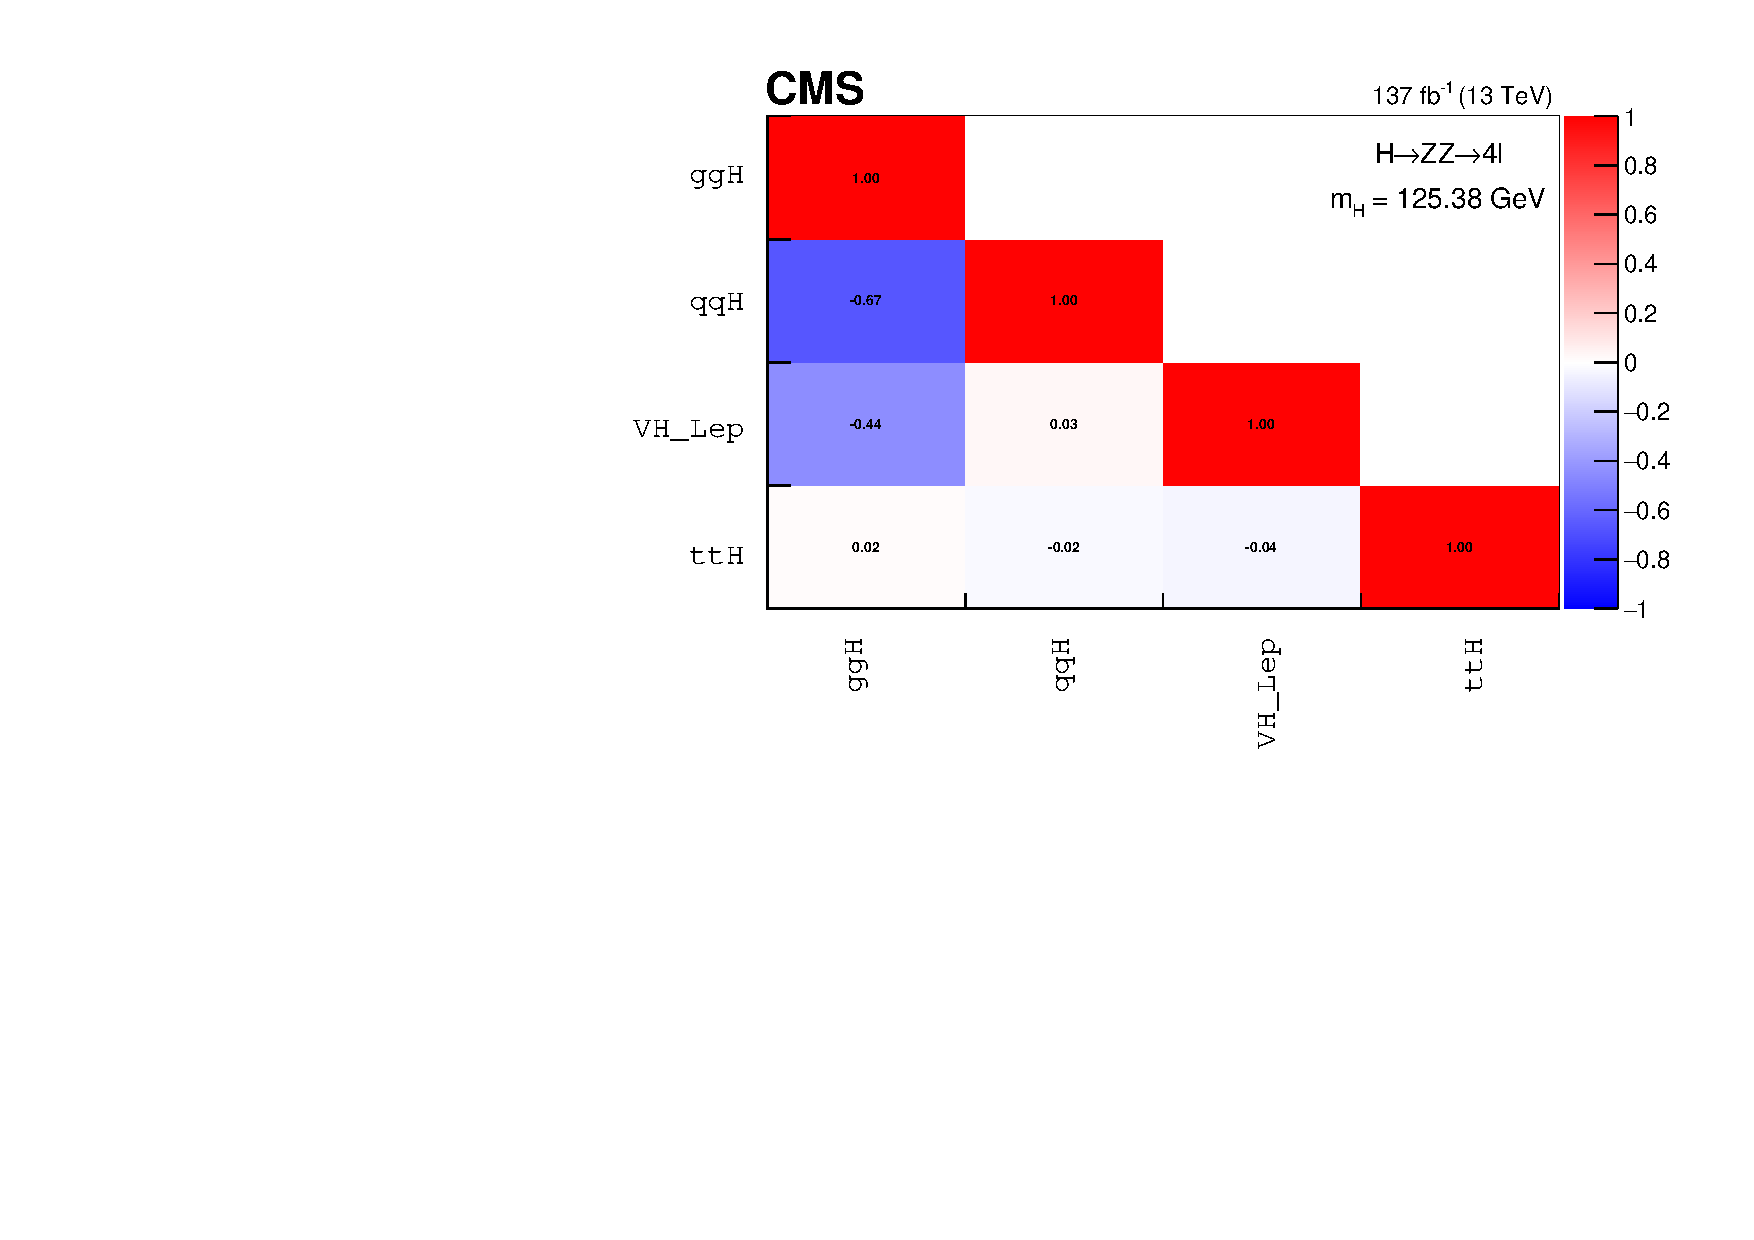
\includegraphics[height=0.6\linewidth]{Figures/results/stxs/scov_stxs0_125_38.pdf}
		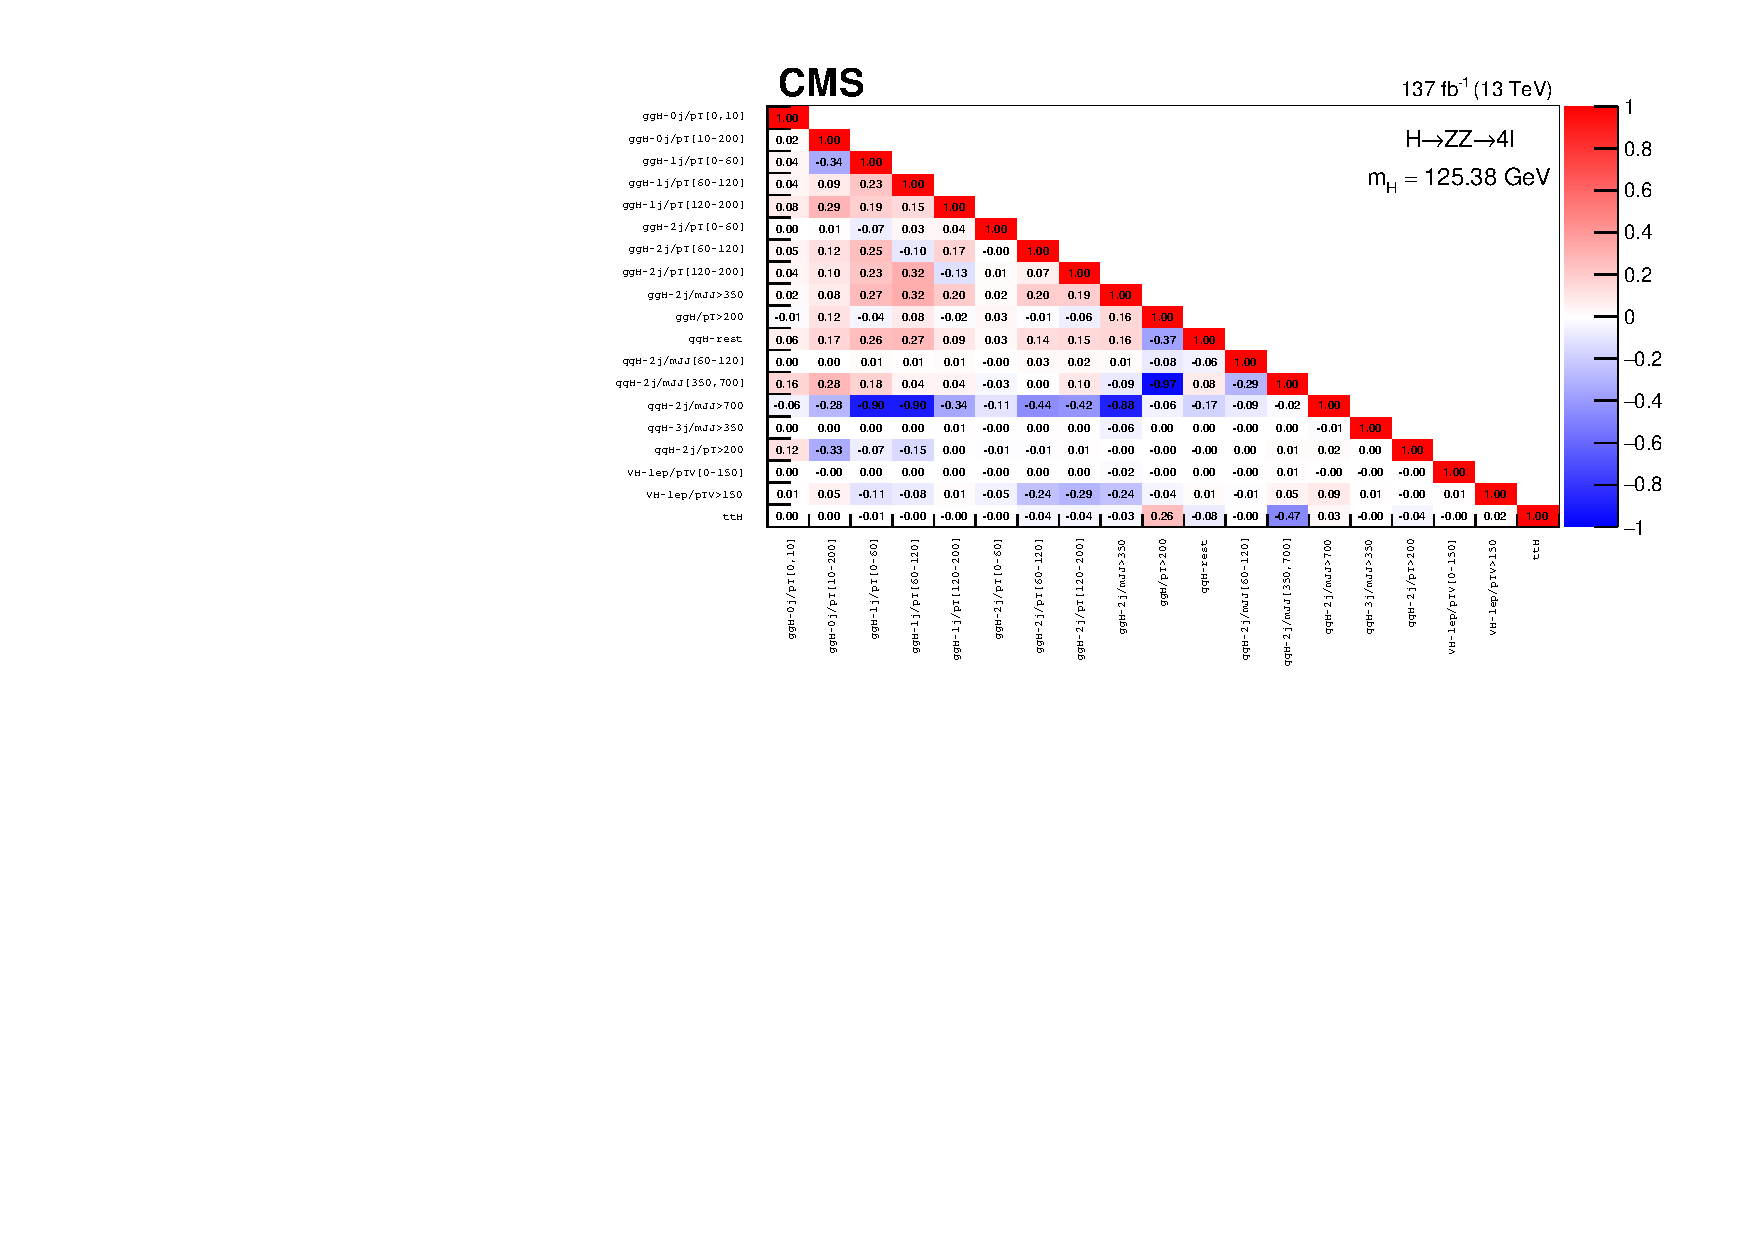
\includegraphics[height=0.6\linewidth]{Figures/results/stxs/scov_stxs1p2_125_38.pdf}
		\caption{The correlation matrices between the measured cross-sections are shown for the stage 0 (left) and the merged stage 1.2 (right).
			\label{fig:corrmatrix}}
	\end{center}
\end{figure}
%%%%%%%%%%%%%%%%%%%%%%%




%In this section we present the results for simplified template cross sections Stage 1.1, a measurement strategy detailed in the CERN Yellow Report 4 of the LHC-HXSWG~\cite{YR4}. The reduced stage 1.1 bins are measured in forms of signal strength modifier. Figure~\ref{fig:stage1p1_mu} shows the results. The covariance matrix of the fitted results are shown in Figure~\ref{fig:cov} 

%%=======
%\begin{figure}[!htb]
%        \vspace*{0.3cm}
%        \begin{center}
%                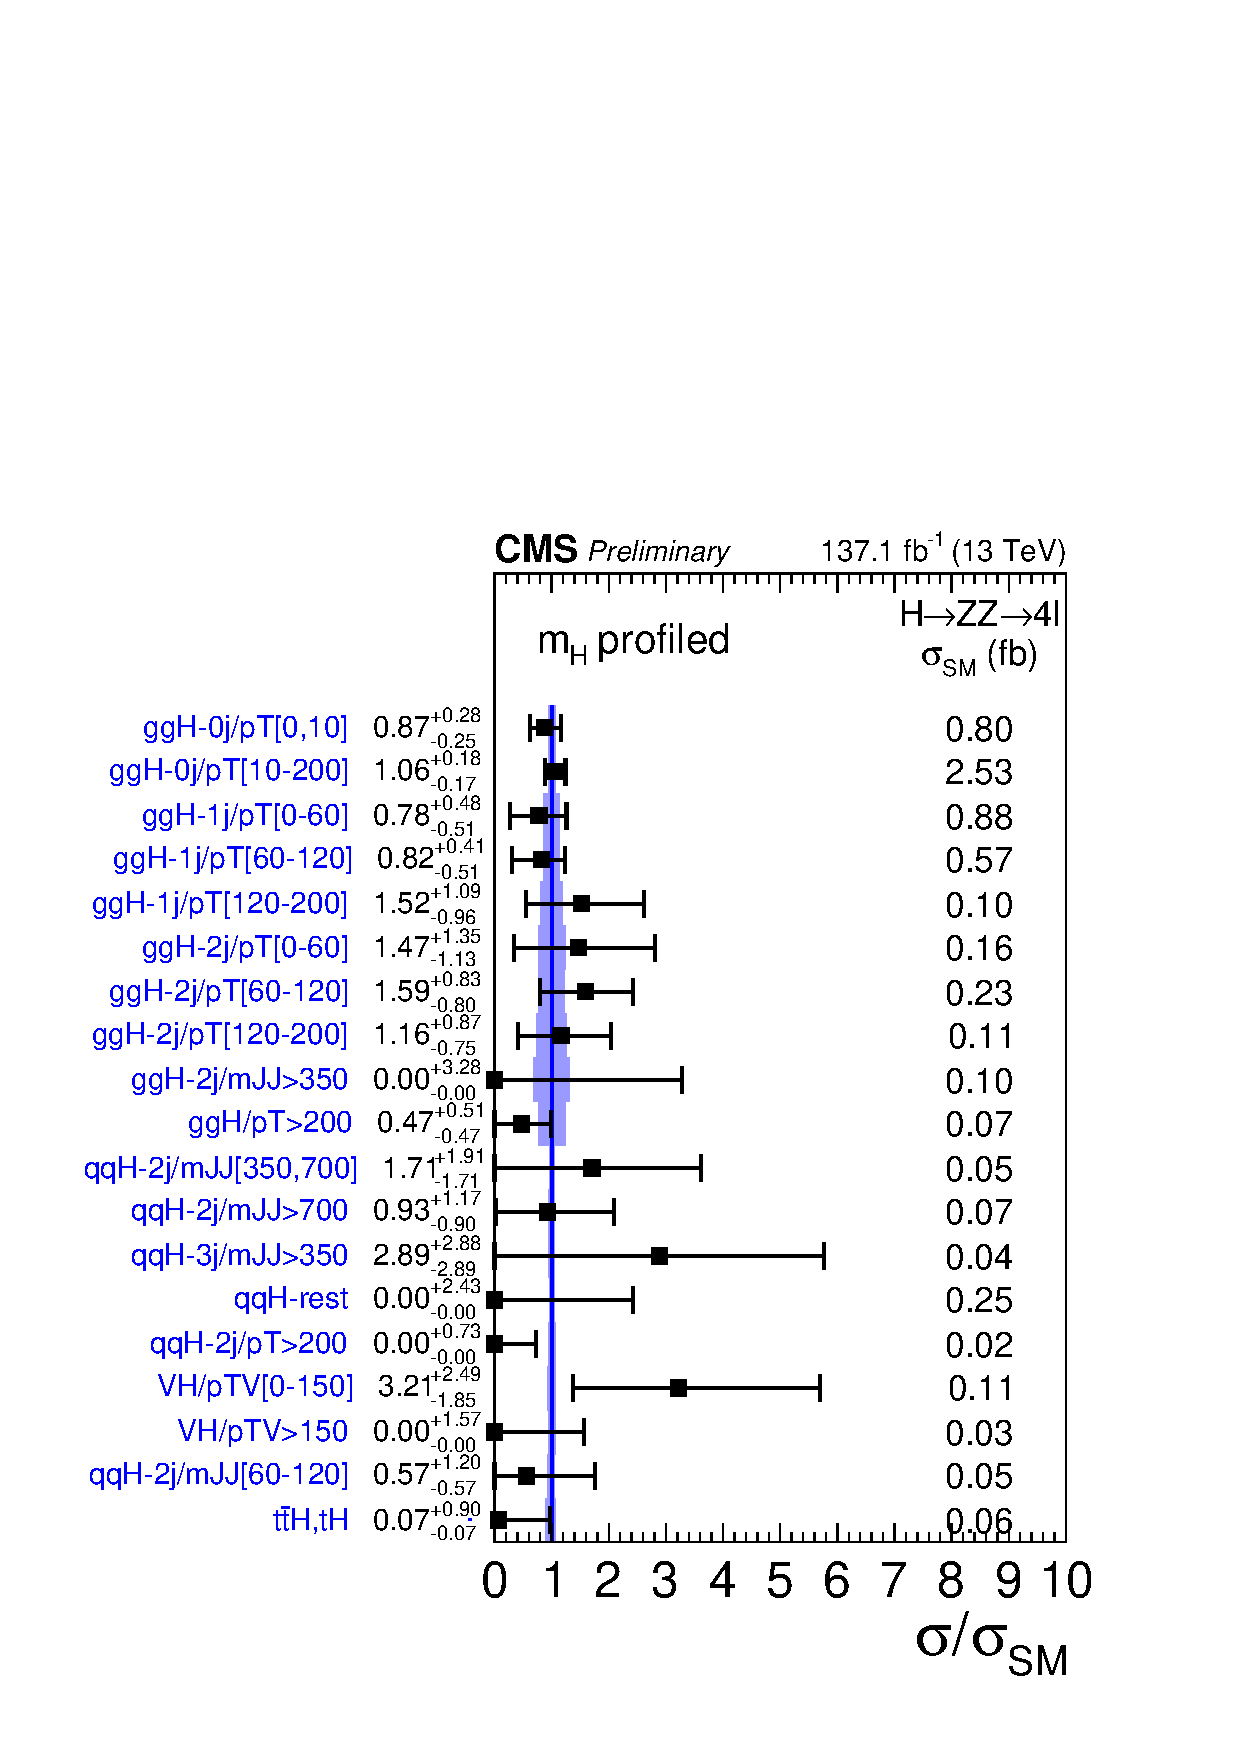
\includegraphics[width=0.8\textwidth]{Figures/results/stxs/mu_stage1_xsec.pdf}
%                \caption{The ratios between measured cross sections and the SM prediction for stage1.1 bins, the \mH is profiled. The band around the vertical band shows the theoretical uncertainties on the SM cross section predictions for each stage 1.1 bin.}
%                \label{fig:stage1p1_mu}}
%        \end{center}
%\end{figure}
%=======

%=======
%\begin{figure}[!htb]
%        \vspace*{0.3cm}
%        \begin{center}
%                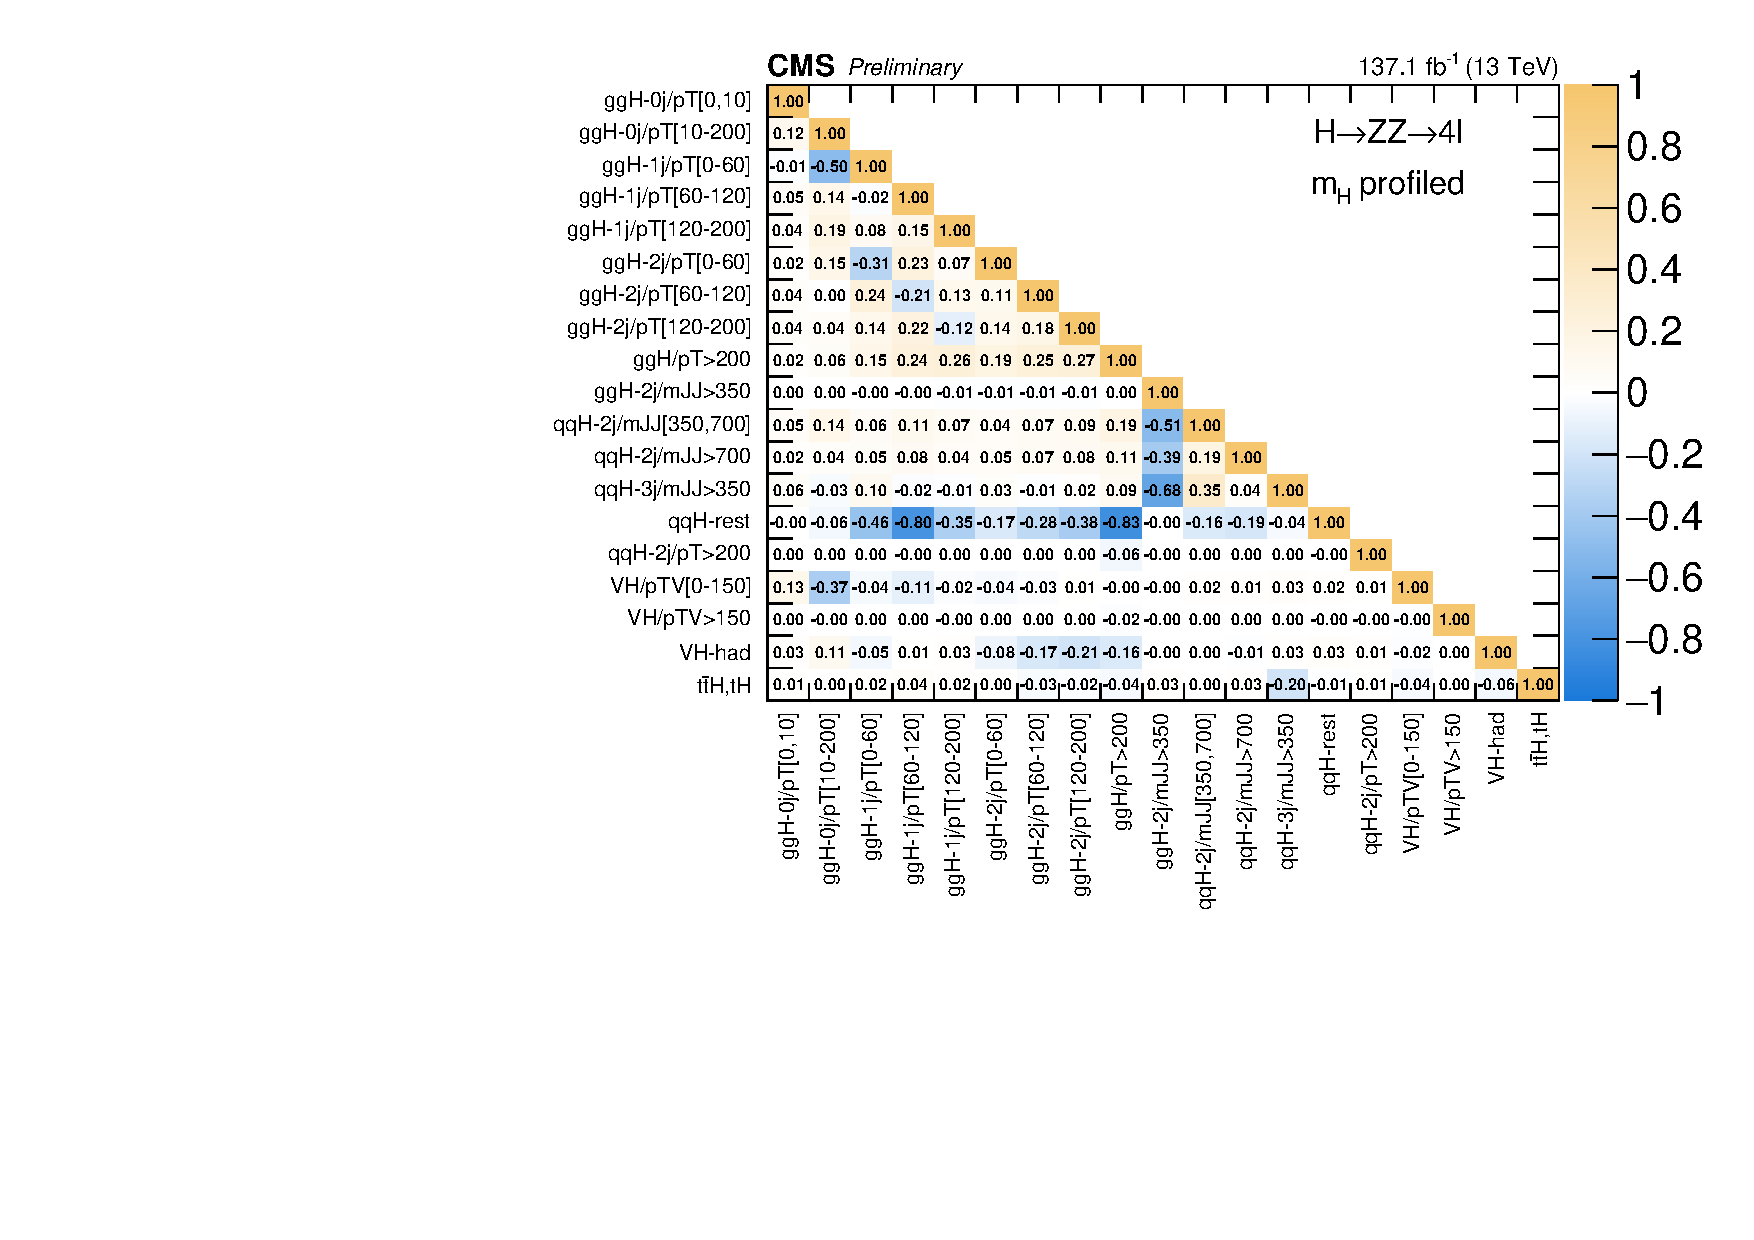
\includegraphics[width=0.8\textwidth]{Figures/results/stxs/scov_stage1.pdf}
%                \caption{Covariance matrix of the fitted signal strength.}
%                \label{fig:cov}}
%        \end{center}
%\end{figure}
%=======
 

\clearpage 

%\subsection{Differential Cross Sections}
\subsection{Differential Cross Sections and EFT interpretations}
\label{sec:diff_xsec}
\textbf{FIXME: Results to be updated with final processing}

\subsubsection{Fiducial Volume Definition}

The fiducial volume is defined to match closely the reconstruction level selection and is very similar to the definition
used in Refs.~\cite{CMSH4lFiducial8TeV}. With respect to the Run 1 analysis, 
the leptons are defined as ``dressed'' leptons rather than Born level leptons. 
Leptons are dressed by adding the four-momenta of leptons within $\Delta R<0.3$ to the bare leptons.  
The fiducial lepton isolation criteria is also updated to match the Run 2 reconstruction level isolation. Leptons are considered isolated at generator level if the sum pt of particles within a cone  $\Delta R<0.3$ is less than 0.35.
The fiducial volume definition can be seen in Table~\ref{tab:FidDef}. 
The fiducial volume acceptance for various SM production modes can be seen in Table~\ref{tab:summarySM}.

\begin{table}[!h!tb]
	\begin{center}
		\small
		\caption{
			Summary of requirements and selections used in the definition of the fiducial phase space for the $\Hllll$ cross section measurements.
			\label{tab:FidDef}
		}
		\begin{tabular}{|lc|} 
			\hline %---------------------------------------------------------
			\hline %---------------------------------------------------------
			\multicolumn{2}{|c|}{\textbf{Requirements for the $\Hllll$ fiducial phase space}} \\
			\hline %---------------------------------------------------------
			\hline %---------------------------------------------------------
			\multicolumn{2}{|c|}{Lepton kinematics and isolation} \\
			\hline %---------------------------------------------------------
			\vspace{-0.4cm} & \\
			leading lepton $\pt$ & $\pt  > 20$~GeV \\ 
			\vspace{-0.4cm} & \\
			next-to-leading lepton $\pt$ & $\pt  > 10$~GeV \\ 
			\vspace{-0.4cm} & \\
			additional electrons (muons) $\pt$ & $\pt  > 7(5)$~GeV \\ 
			\vspace{-0.4cm} & \\
			pseudorapidity of electrons (muons) & $|\eta| < 2.5(2.4)$ \\ 
			\vspace{-0.4cm} & \\
			$\pt$ sum of all stable particles within $\Delta R < 0.3$ from lepton & less than $0.35 \cdot \pt$ \\ 
			%\vspace{-0.4cm} & \\
			\hline %---------------------------------------------------------
			\hline %---------------------------------------------------------
			\multicolumn{2}{|c|}{Event topology} \\
			\hline %---------------------------------------------------------
			\multicolumn{2}{|l|}{existence of at least two SFOS lepton pairs, where leptons satisfy criteria above} \\
			%\vspace{-0.4cm} & \\
			inv. mass of the Z$_1$ candidate & $40 \GeV < m($Z$_{1}$)$< 120 \GeV$ \\ 
			\vspace{-0.4cm} & \\
			inv. mass of the Z$_2$ candidate & $12 \GeV < m($Z$_{2}$)$< 120 \GeV$ \\ 
			\vspace{-0.4cm} & \\
			distance between selected four leptons & $\Delta R(\ell_{i}\ell_{j})>0.02$ for any $i\neq j$  \\ 
			\vspace{-0.4cm} & \\
			inv. mass of any opposite sign lepton pair & m$(\ell^{+}\ell'^{-})>4 \GeV$ \\ 
			\vspace{-0.4cm} & \\
			inv. mass of the selected four leptons & $105 \GeV < m_{4\ell} < 140 \GeV$  \\ 
			\vspace{-0.4cm} & \\
			\multicolumn{2}{|l|}{the selected four leptons must originate from the $\Hllll$ decay} \\
			\hline %---------------------------------------------------------
			\hline %---------------------------------------------------------
		\end{tabular}
		\normalsize
	\end{center}
\end{table}

\subsubsection{Measurement Strategy}

We measure the integrated and differential fiducial cross section for $pp\to$H$\to4\ell$ by performing a maximum likelihood fit of the signal and background parameterisations to the observed $4\ell$ mass distribution, $N_{\mathrm{obs}}(m_{4\ell})$, and the fiducial cross section ($\sigma_{\mathrm{fid}}$) is directly extracted from the fit. The systematic uncertainties are included in the form of nuisance parameters and are effectively integrated out in the fit procedure. The results are obtained using an asymptotic approach~\cite{LHC-HCG} with a test statistic based on the profile likelihood ratio~\cite{Cowan:2010js}. This procedure for the unfolding of the detector effects from the observed distributions is the same as in Refs.~\cite{CMSH4lFiducial8TeV}~and~\cite{CMSHggFiducial8TeV}. In the case of the differential cross section measurements,  the finite efficiencies and resolution effects are encoded in a detector response matrix which describes how events migrate from a given observable bin at the fiducial level to a given bin at the reconstruction level. This matrix is diagonally dominant, with sizeable off-diagonal elements for observables involving jets.

Following the models for signal and background contributions described above, the number of expected events in each final state f and in each bin $i$ of a considered observable is expressed as a function of $m_{4\ell}$ given by: 
\begin{eqnarray}
\label{eqn:m4l}
\begin{aligned}
N_{\mathrm{obs}}^{\mathrm{f},i}(m_{4\ell}) &= N_{\mathrm{fid}}^{\mathrm{f},i}(m_{4\ell})+N_{\mathrm{nonfid}}^{\mathrm{f},i}(m_{4\ell})+N_{\mathrm{nonres}}^{\mathrm{f},i}(m_{4\ell})+N_{\mathrm{bkg}}^{\mathrm{f},i}(m_{4\ell}) \\
&=\epsilon_{i,j}^{\mathrm{f}} \cdot \left(1+f_{\rm nonfid}^{\mathrm{f},i} \right)\cdot\sigma_{\mathrm{fid}}^{\mathrm{f},j} \cdot \mathcal{L}\cdot\mathcal{P}_{\mathrm{res}}(m_{4\ell}) \\
&~~~~~+ N_{\mathrm{nonres}}^{\mathrm{f},i}\cdot\mathcal{P}_{\mathrm{nonres}}(m_{4\ell})+N_{\mathrm{bkg}}^{\mathrm{f},i}\cdot\mathcal{P}_{\mathrm{bkg}}(m_{4\ell}),
\end{aligned}
\end{eqnarray}

The parameter $\sigma_{\mathrm{fid}}^{\mathrm{f},j}$ is the signal cross section in bin $j$ of the fiducial phase space, and it is the parameter extracted from the measurement. 

The shape of the resonant signal contribution, $\mathcal{P}_{\mathrm{res}}(m_{4\ell})$, is described by a double-sided Crystal Ball function as described in Section~\ref{sec:signalshapes} whose normalisation is proportional to the fiducial cross section. The shape of the non-resonant signal contribution, $\mathcal{P}_{\mathrm{nonres}}(m_{4\ell})$, which arises from WH, ZH, and $\ttH$ production where one of the leptons from the Higgs boson decay is lost or not selected, is empirically modelled by a Landau distribution whose shape parameters are constrained in the fit to be within a range determined from simulation. This contribution is treated as a background and hereafter we will refer to this contribution as the ``non-resonant signal'' contribution.

The $\epsilon_{i,j}^{\mathrm{f}}$ represents the detector response matrix that maps the number of expected events in a given observable bin $j$ at the fiducial level to the number of expected events in the bin $i$ at the reconstruction level. The $f_{\rm nonfid}^{i}$ fraction describes the ratio of the non-fiducial and fiducial signal contribution in bin $i$ at the reconstruction level.  The efficiency is measured using signal simulation samples and corrected for residual differences between data and simulation. In the case of the integrated fiducial cross section measurement the efficiencies reudce to a single values.

An  additional resonant contribution arises from events which are reconstructed but which do not originate from the fiducial phase space. These events are due to detector effects which cause differences between the quantities used for the fiducial phase space definition and the analagous quantities are the reconstruction level. This contribution is treated as background and is referred to as the ``non-fiducial signal'' contribution. The shape of these events is verified using simulation to be identical to the shape of the fiducial signal and its normalisation is fixed to be a fraction of the fiducial signal component. The value of this fraction, which we denote by $f_{\mathrm{nonfid}}$, which has been determined from simulation for each of the studied signal models. 

The variation between different models of the factor in the final column of Table~\ref{tab:summarySM}, $(1+f_{\rm{nonfid}})\epsilon$, is directly related to the model dependence of the measurement. 
The model dependence is defined as the variation of the factor $(1+f_{\rm{nonfid}})\epsilon$ when the relative fraction of each the production modes are varied within there experimental constraints. An increase in model dependence compared to Run 1 is observed when using the ZZ candidate selection at reconstruction level where the the candidate with the best $\KD$ discriminant value is chosen. Therefore the fiducial cross section measurement is performed with a different event selection algorithm than the other measurements, namely that the ZZ candidate selection is made using the same algorithm as in Run 1. 

\begin{table}[!h!tb]
	\begin{center}
		\small
		\caption{
			Summary of different Standard Model signal models. The MC samples are from 2016 production.
			\label{tab:summarySM}
		}
		\begin{tabular}{|l|c|c|c|c|} \hline \hline 
			\textbf{Signal process} & $\mathcal{A}_{\rm fid}$ & $\epsilon$ & $f_{\rm nonfid}$  & $(1+f_{\rm nonfid})\epsilon$ \\ \hline \hline 
			\multicolumn{5}{|c|}{Individual Higgs boson production modes} \\ \hline 
			gg$\rightarrow$H ({\sc powheg})& 0.398 & 0.592 $\pm$ 0.001 & 0.049 $\pm$ 0.001 & 0.621 $\pm$ 0.001 \\ 
			%gg$\rightarrow$H ({\sc minloHJ NNLOPS})& 0.442 & 0.595 $\pm$ 0.001 & 0.049 $\pm$ 0.001 & 0.624 $\pm$ 0.001 \\ 
			VBF ({\sc powheg})& 0.445 & 0.601 $\pm$ 0.002 & 0.038 $\pm$ 0.001 & 0.624 $\pm$ 0.002 \\ 
			WH ({\sc powheg+minlo})& 0.314 & 0.577 $\pm$ 0.002 & 0.068 $\pm$ 0.001 & 0.616 $\pm$ 0.002 \\ 
			ZH ({\sc powheg+minlo})& 0.342 & 0.592 $\pm$ 0.003 & 0.071 $\pm$ 0.002 & 0.634 $\pm$ 0.003 \\ 
			ttH ({\sc powheg})& 0.311 & 0.572 $\pm$ 0.003 & 0.136 $\pm$ 0.003 & 0.650 $\pm$ 0.004 \\ 
			\hline \hline
		\end{tabular}
		\normalsize
	\end{center}
\end{table}



\begin{table}[!h!tb]
	\begin{center}
		\small
		\caption{
			Summary of different Standard Model signal models. The MC samples are from 2017 production.
			\label{tab:summarySM}
		}
		\begin{tabular}{|l|c|c|c|c|} \hline \hline 
			\textbf{Signal process} & $\mathcal{A}_{\rm fid}$ & $\epsilon$ & $f_{\rm nonfid}$  & $(1+f_{\rm nonfid})\epsilon$ \\ \hline \hline 
			\multicolumn{5}{|c|}{Individual Higgs boson production modes} \\ \hline 
 gg$\rightarrow$H ({\sc powheg}) & 0.404 $\pm$ 0.001 & 0.593 $\pm$ 0.001 & 0.054 $\pm$ 0.001 & 0.625 $\pm$ 0.001 \\ 
 VBF ({\sc powheg}) & 0.443 $\pm$ 0.001 & 0.605 $\pm$ 0.002 & 0.045 $\pm$ 0.001 & 0.632 $\pm$ 0.002 \\ 
 WH ({\sc powheg+minlo}) & 0.329 $\pm$ 0.001 & 0.589 $\pm$ 0.002 & 0.080 $\pm$ 0.001 & 0.637 $\pm$ 0.002 \\ 
 ZH ({\sc powheg+minlo}) & 0.341 $\pm$ 0.002 & 0.593 $\pm$ 0.003 & 0.083 $\pm$ 0.002 & 0.643 $\pm$ 0.004 \\ 
 ttH ({\sc powheg}) & 0.316 $\pm$ 0.002 & 0.597 $\pm$ 0.003 & 0.172 $\pm$ 0.004 & 0.700 $\pm$ 0.004 \\ 
			\hline \hline
		\end{tabular}
		\normalsize
	\end{center}
\end{table}


\begin{table}[!h!tb]
	\begin{center}
		\small
		\caption{
			Summary of different Standard Model signal models. The MC samples are from 2018 production. {\color{red} FIXME: Scale factors not yet applied}
			\label{tab:summarySM}
		}
		\begin{tabular}{|l|c|c|c|c|} \hline \hline 
			\textbf{Signal process} & $\mathcal{A}_{\rm fid}$ & $\epsilon$ & $f_{\rm nonfid}$  & $(1+f_{\rm nonfid})\epsilon$ \\ \hline \hline 
			\multicolumn{5}{|c|}{Individual Higgs boson production modes} \\ \hline 
 gg$\rightarrow$H ({\sc powheg})  & 0.403 $\pm$ 0.001 & 0.630 $\pm$ 0.001 & 0.055 $\pm$ 0.001 & 0.664 $\pm$ 0.001 \\ 
 VBF ({\sc powheg})  & 0.443 $\pm$ 0.001 & 0.645 $\pm$ 0.002 & 0.043 $\pm$ 0.001 & 0.673 $\pm$ 0.002 \\ 
 WH ({\sc powheg+minlo})  & 0.330 $\pm$ 0.001 & 0.632 $\pm$ 0.002 & 0.075 $\pm$ 0.001 & 0.679 $\pm$ 0.002 \\ 
 ZH ({\sc powheg+minlo})  & 0.338 $\pm$ 0.002 & 0.638 $\pm$ 0.003 & 0.086 $\pm$ 0.003 & 0.693 $\pm$ 0.004 \\ 
 ttH ({\sc powheg})  & 0.314 $\pm$ 0.002 & 0.620 $\pm$ 0.003 & 0.184 $\pm$ 0.004 & 0.733 $\pm$ 0.004 \\
			\hline \hline
		\end{tabular}
		\normalsize
	\end{center}
\end{table}






Examples of the efficiency matrices for gluon fusion and VBF production can be seen in Fig.~\ref{fig:eff2d}. The matrices for the $\pt_{\rm H}$ and N(jets) observables are shown.

\begin{figure}[!h]
	\centering
	\includegraphics[width=0.32\linewidth]{Figures/results/fiducial/2016/eff2d_ggH_powheg_JHUgen_125_pT4l_2e2mu.pdf}
	\includegraphics[width=0.32\linewidth]{Figures/results/fiducial/2017/eff2d_ggH_powheg_JHUgen_125_pT4l_2e2mu.pdf}
	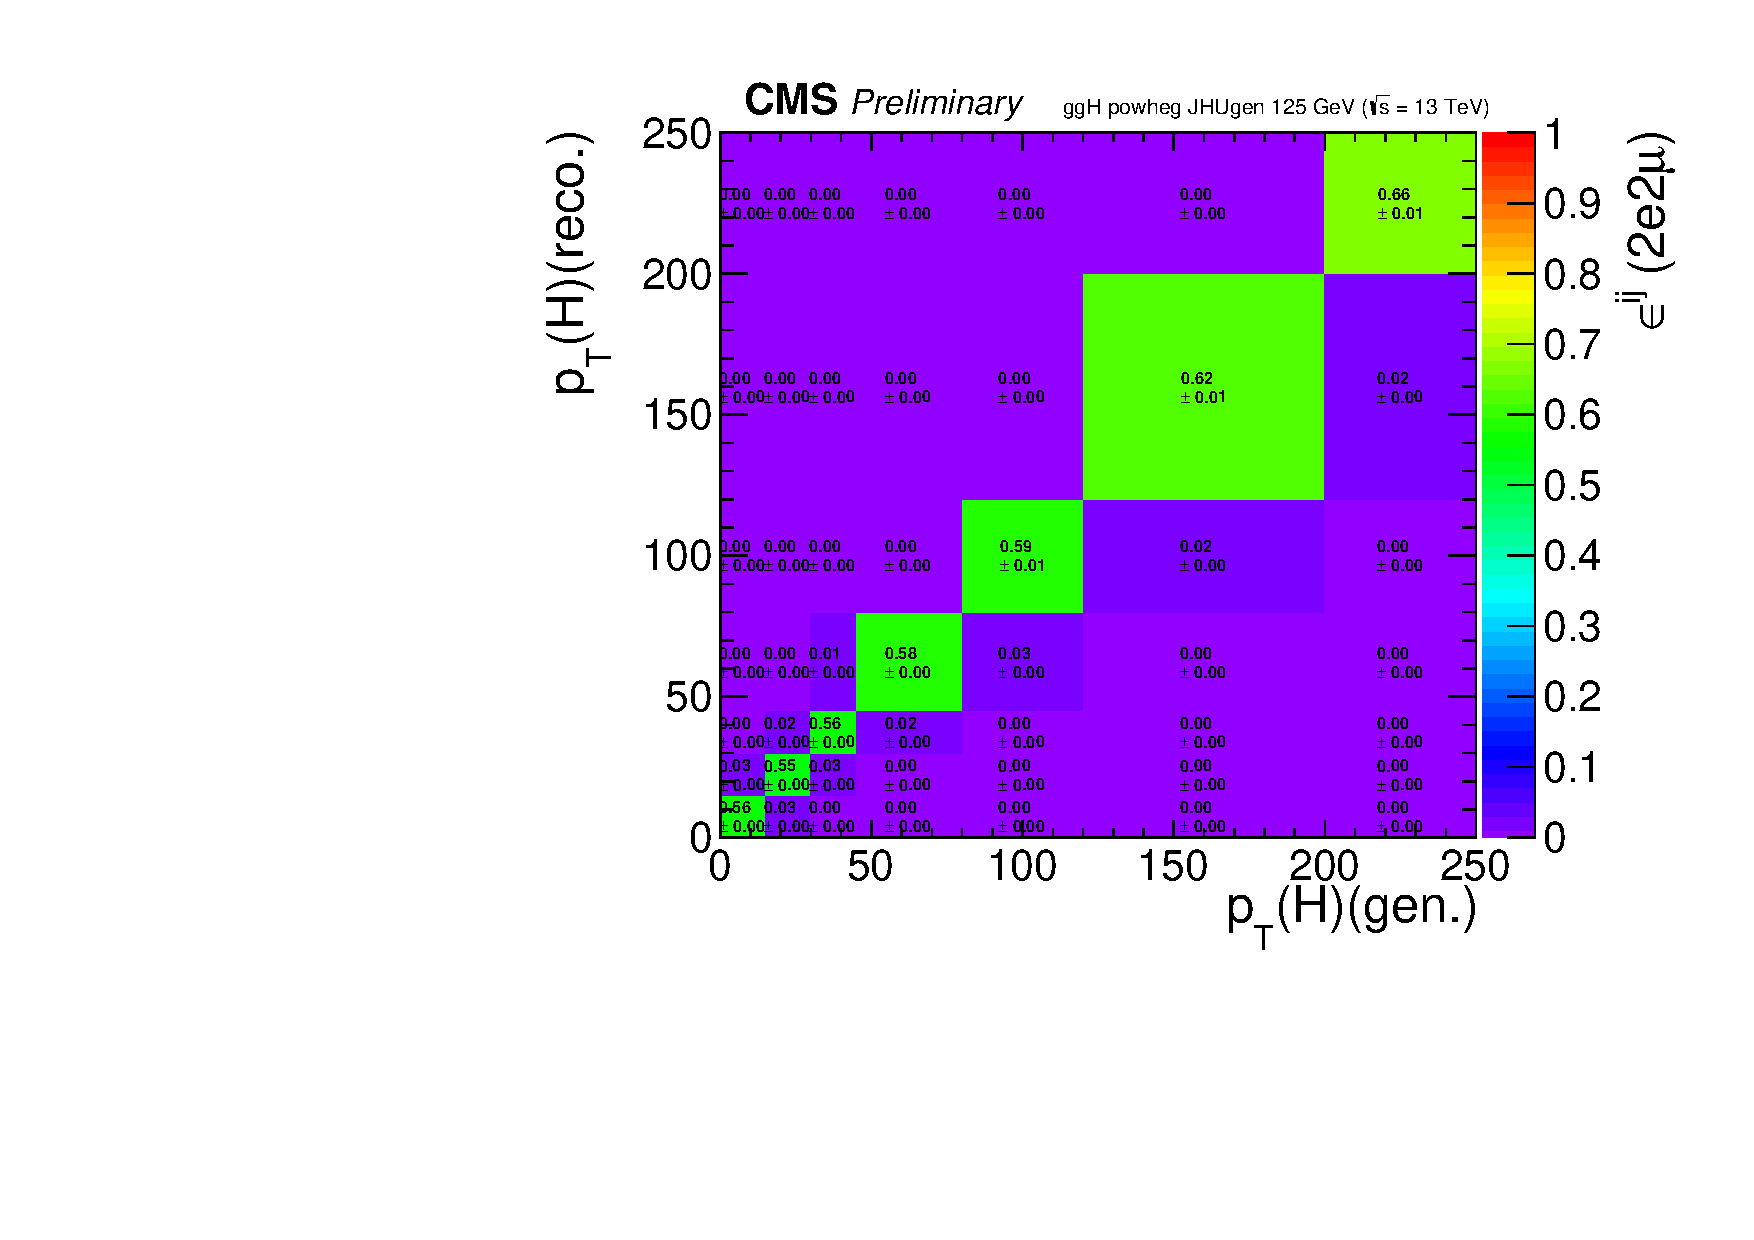
\includegraphics[width=0.32\linewidth]{Figures/results/fiducial/2018/eff2d_ggH_powheg_JHUgen_125_pT4l_2e2mu.pdf} \\
	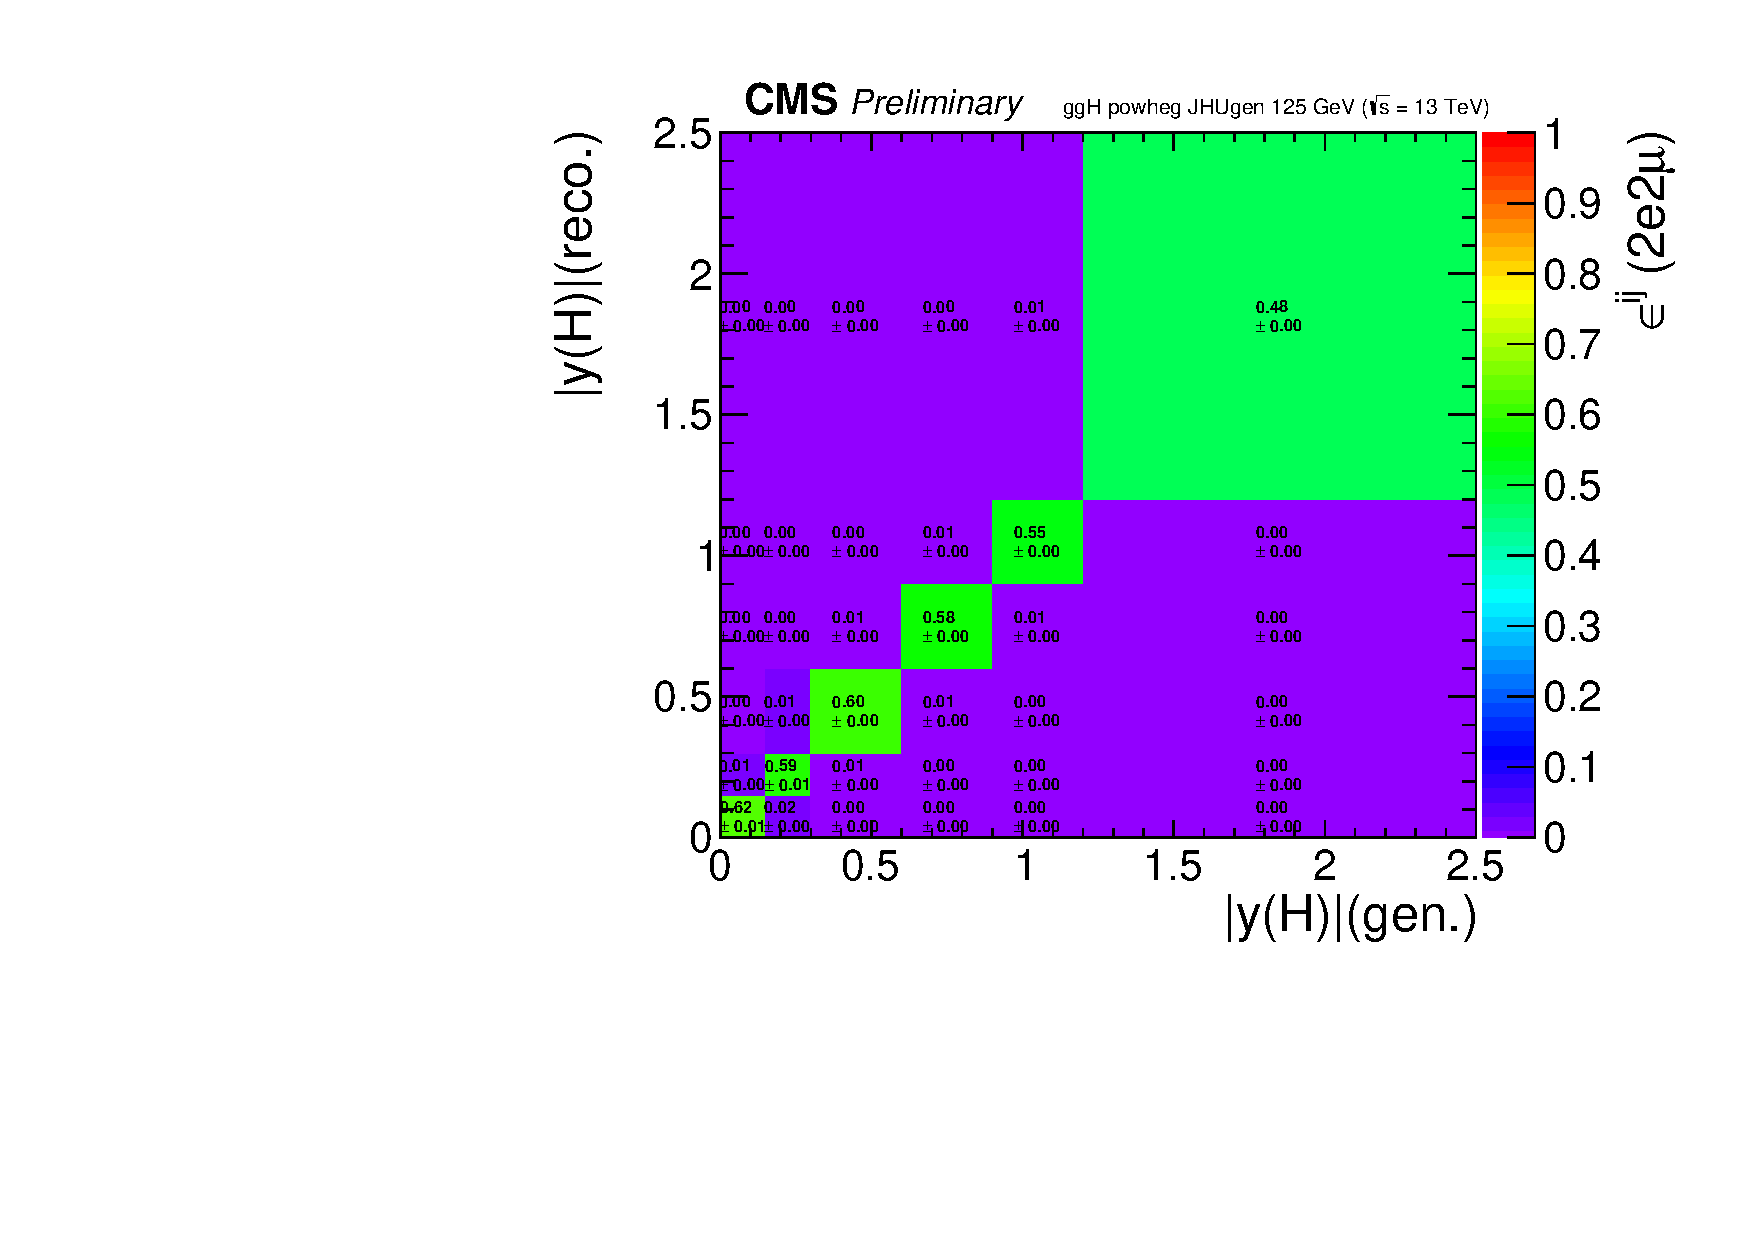
\includegraphics[width=0.32\linewidth]{Figures/results/fiducial/2016/eff2d_ggH_powheg_JHUgen_125_rapidity4l_2e2mu.pdf}
	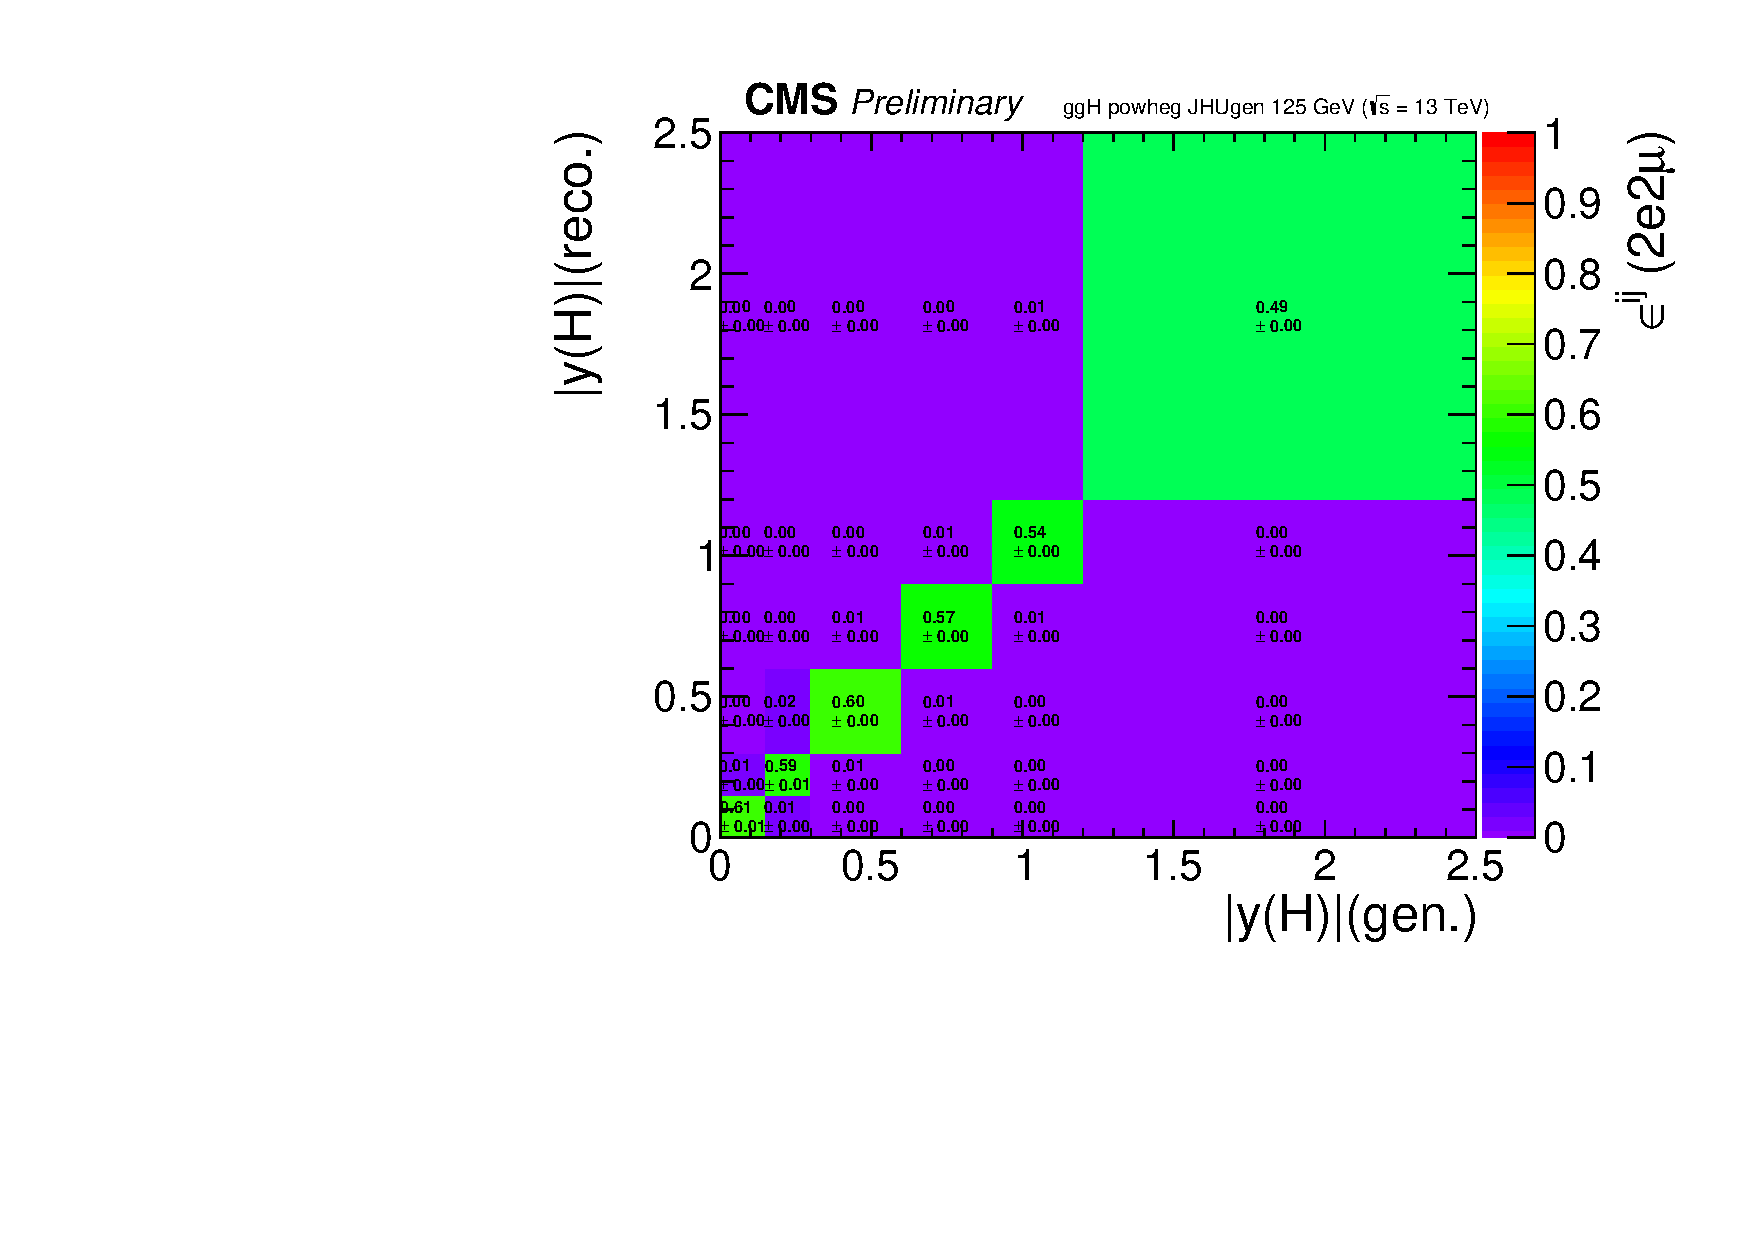
\includegraphics[width=0.32\linewidth]{Figures/results/fiducial/2017/eff2d_ggH_powheg_JHUgen_125_rapidity4l_2e2mu.pdf}
	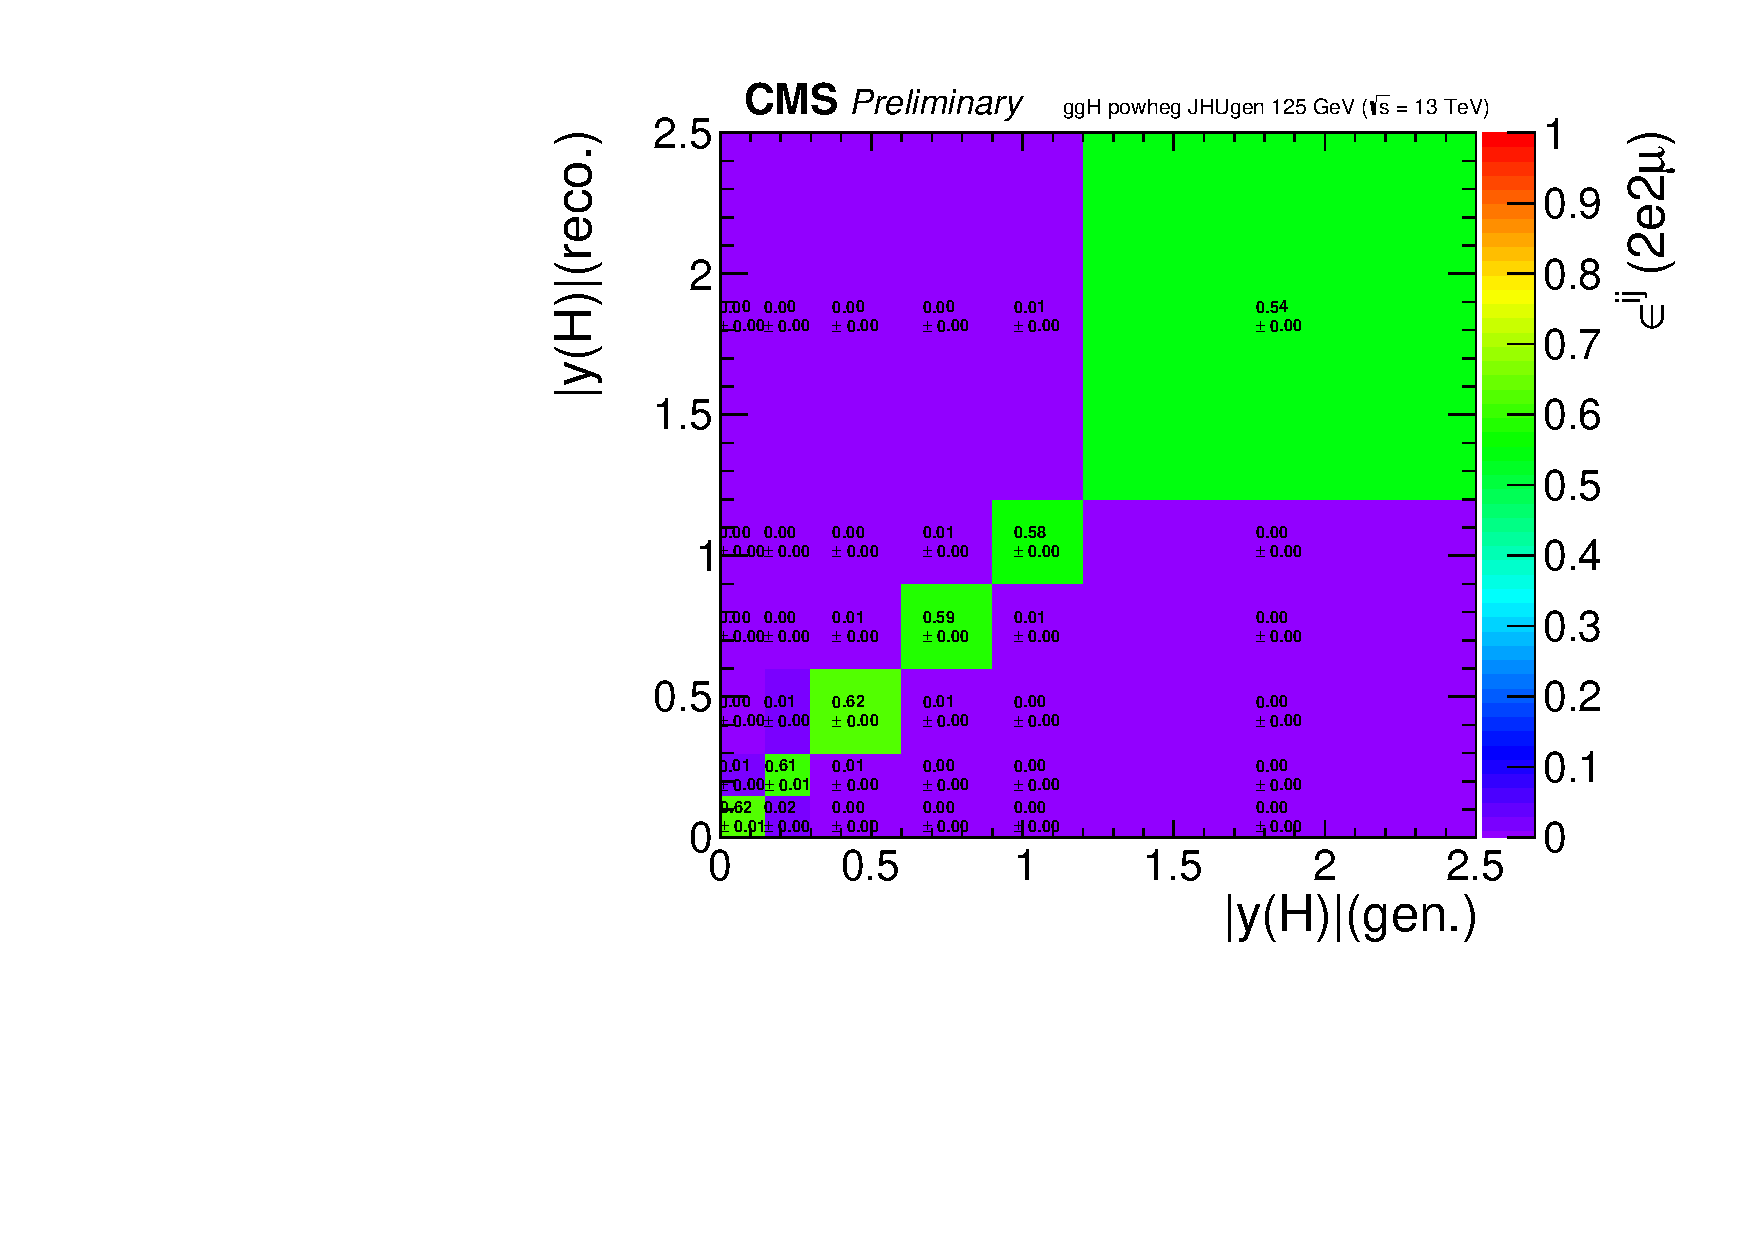
\includegraphics[width=0.32\linewidth]{Figures/results/fiducial/2018/eff2d_ggH_powheg_JHUgen_125_rapidity4l_2e2mu.pdf} \\
	\includegraphics[width=0.32\linewidth]{Figures/results/fiducial/2016/eff2d_ggH_powheg_JHUgen_125_njets_pt30_eta2p5_2e2mu.pdf}
	\includegraphics[width=0.32\linewidth]{Figures/results/fiducial/2017/eff2d_ggH_powheg_JHUgen_125_njets_pt30_eta2p5_2e2mu.pdf}
	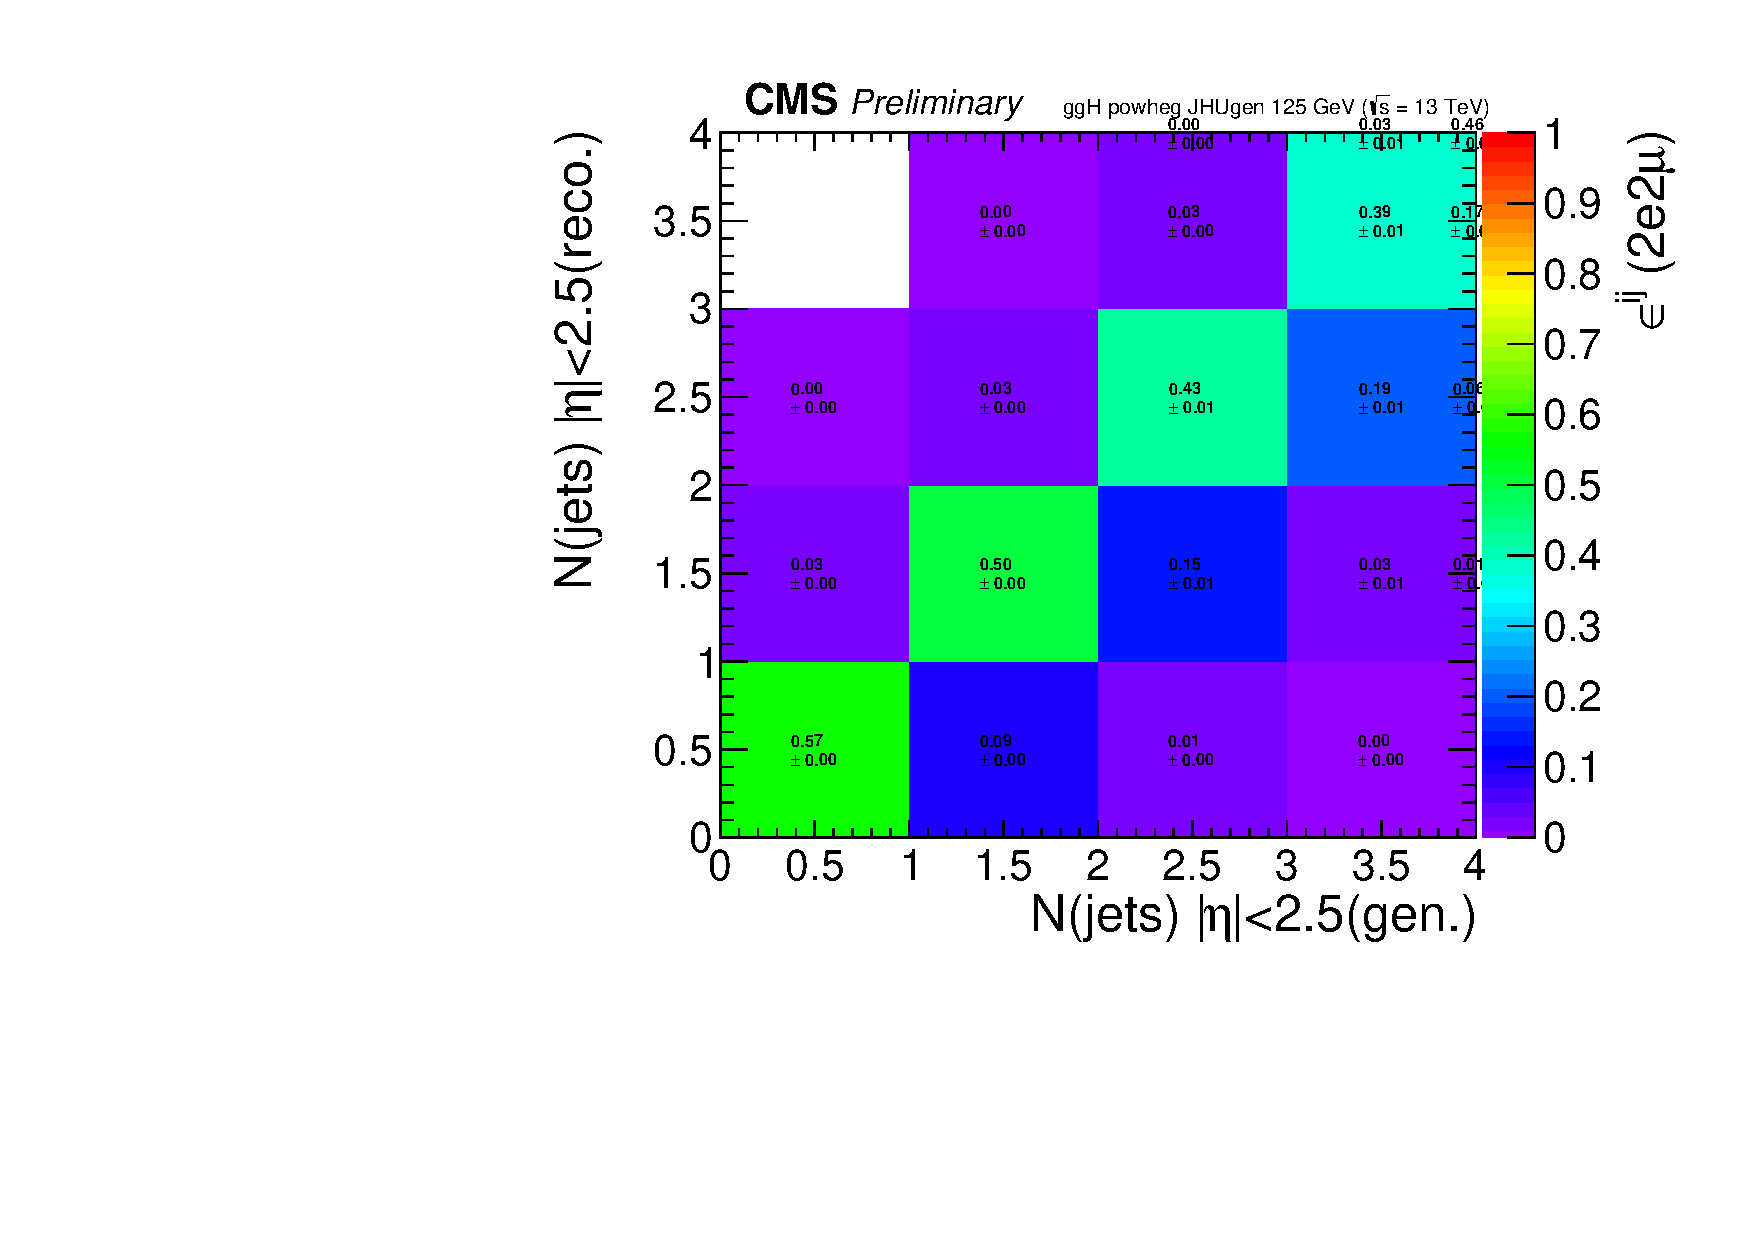
\includegraphics[width=0.32\linewidth]{Figures/results/fiducial/2018/eff2d_ggH_powheg_JHUgen_125_njets_pt30_eta2p5_2e2mu.pdf} 
	
	\caption{Efficiency matrices for the $\pt_{\rm H}$ (top) and $y{\rm H}$ (middle) and N(jets) (bottom) observables for gluon fusion production
		modes in the $2e2\mu$ final state in 2016 (left) 2017 (middle) and 2018 (right). \label{fig:eff2d}}
\end{figure}


\subsubsection{Measurement results}

The result of the simultaneous fit to to the $\mllll$ spectrum is shown for each final state in Fig.~\ref{fig:fiducialfit}. The fiducial cross section using this defintion is measured to be:

\begin{eqnarray}
\label{eqn:fidresult}
2.85^{+0.24}_{-0.23}({\rm stat.})^{+0.15}_{-0.14}({\rm sys.})~{\rm fb}
\end{eqnarray}

This can be compared to the SM expectation of $\sigma_{{\rm fid.}}^{\rm SM}=2.72\pm0.14~{\rm fb}$.

\begin{figure}[!h]
	\centering
	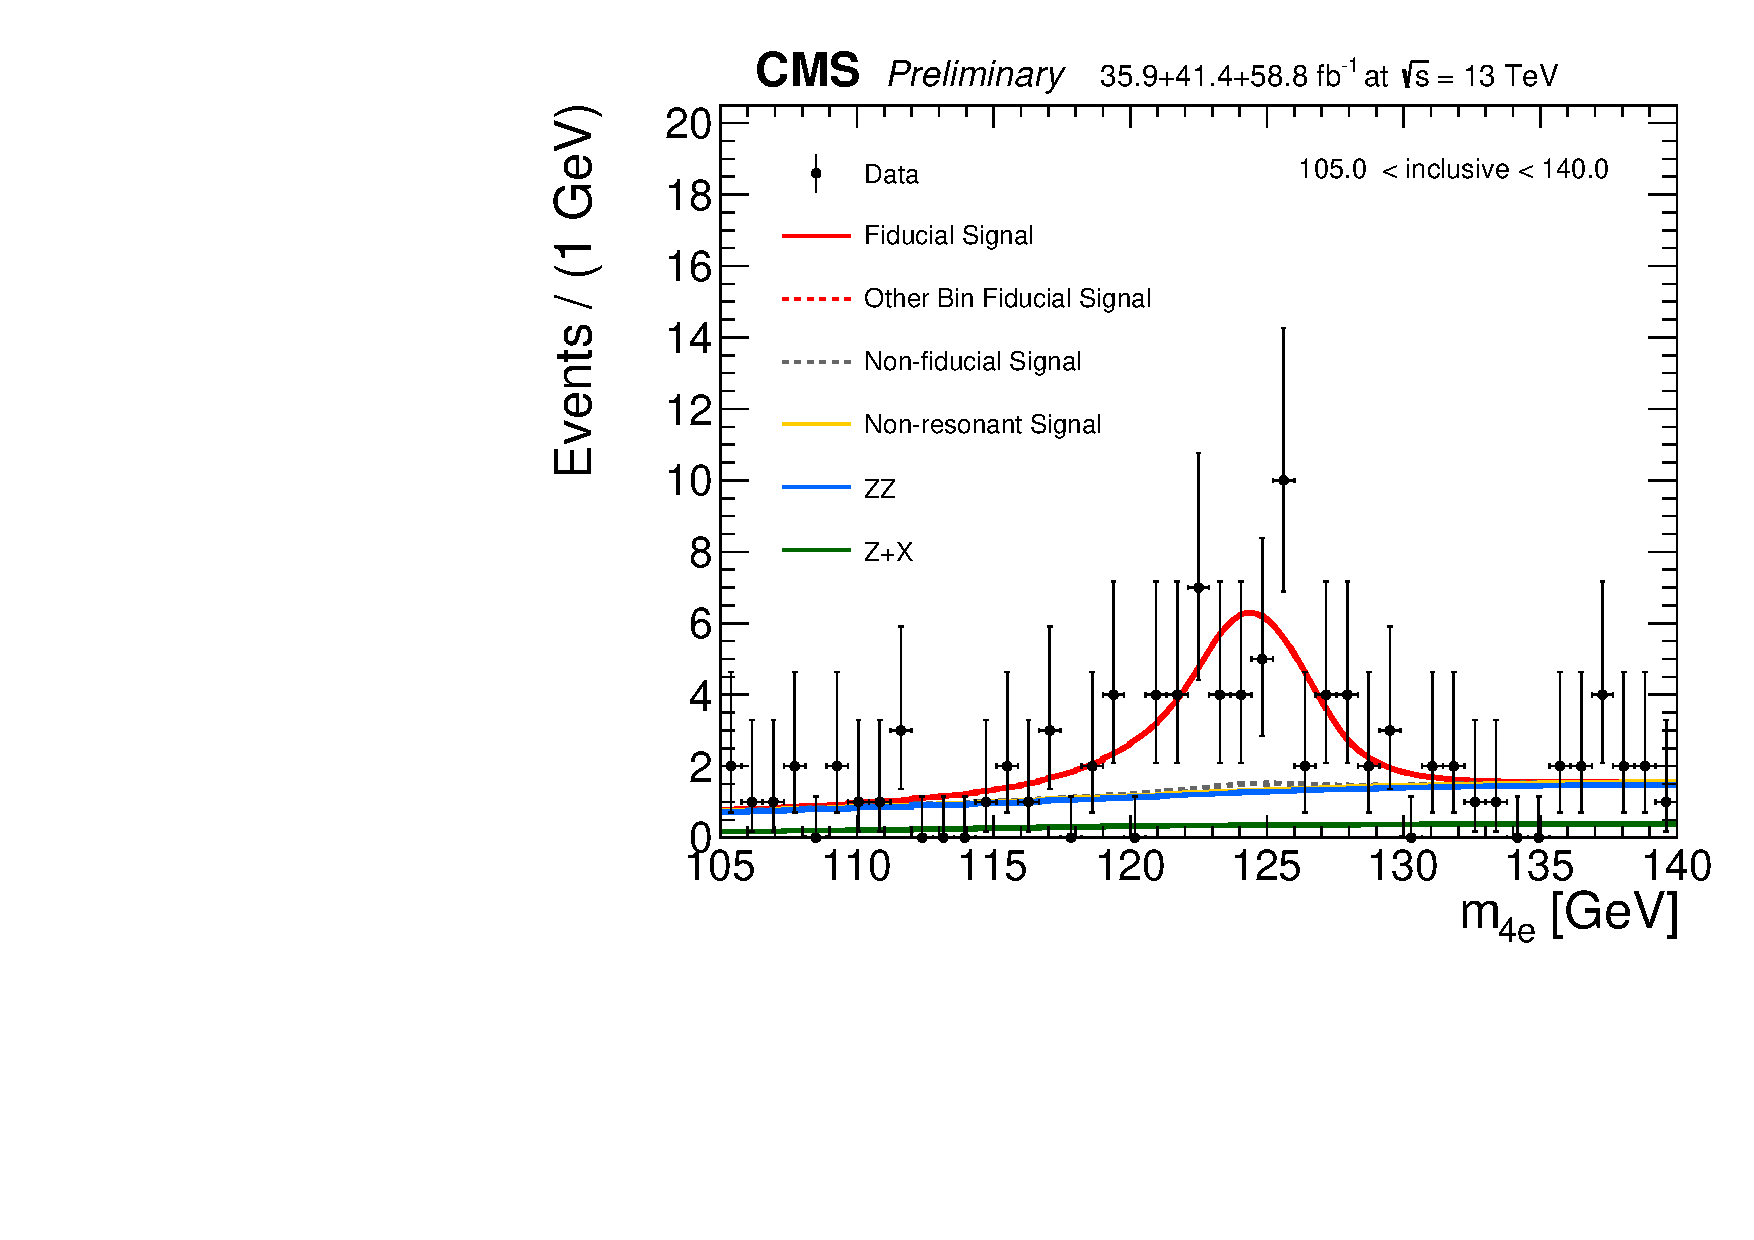
\includegraphics[width=0.45\linewidth]{Figures/results/fiducial/comb/unblind_Feb25/data_unfoldwith_SM_125_v3_mass4l_4e_recobin0.pdf}
	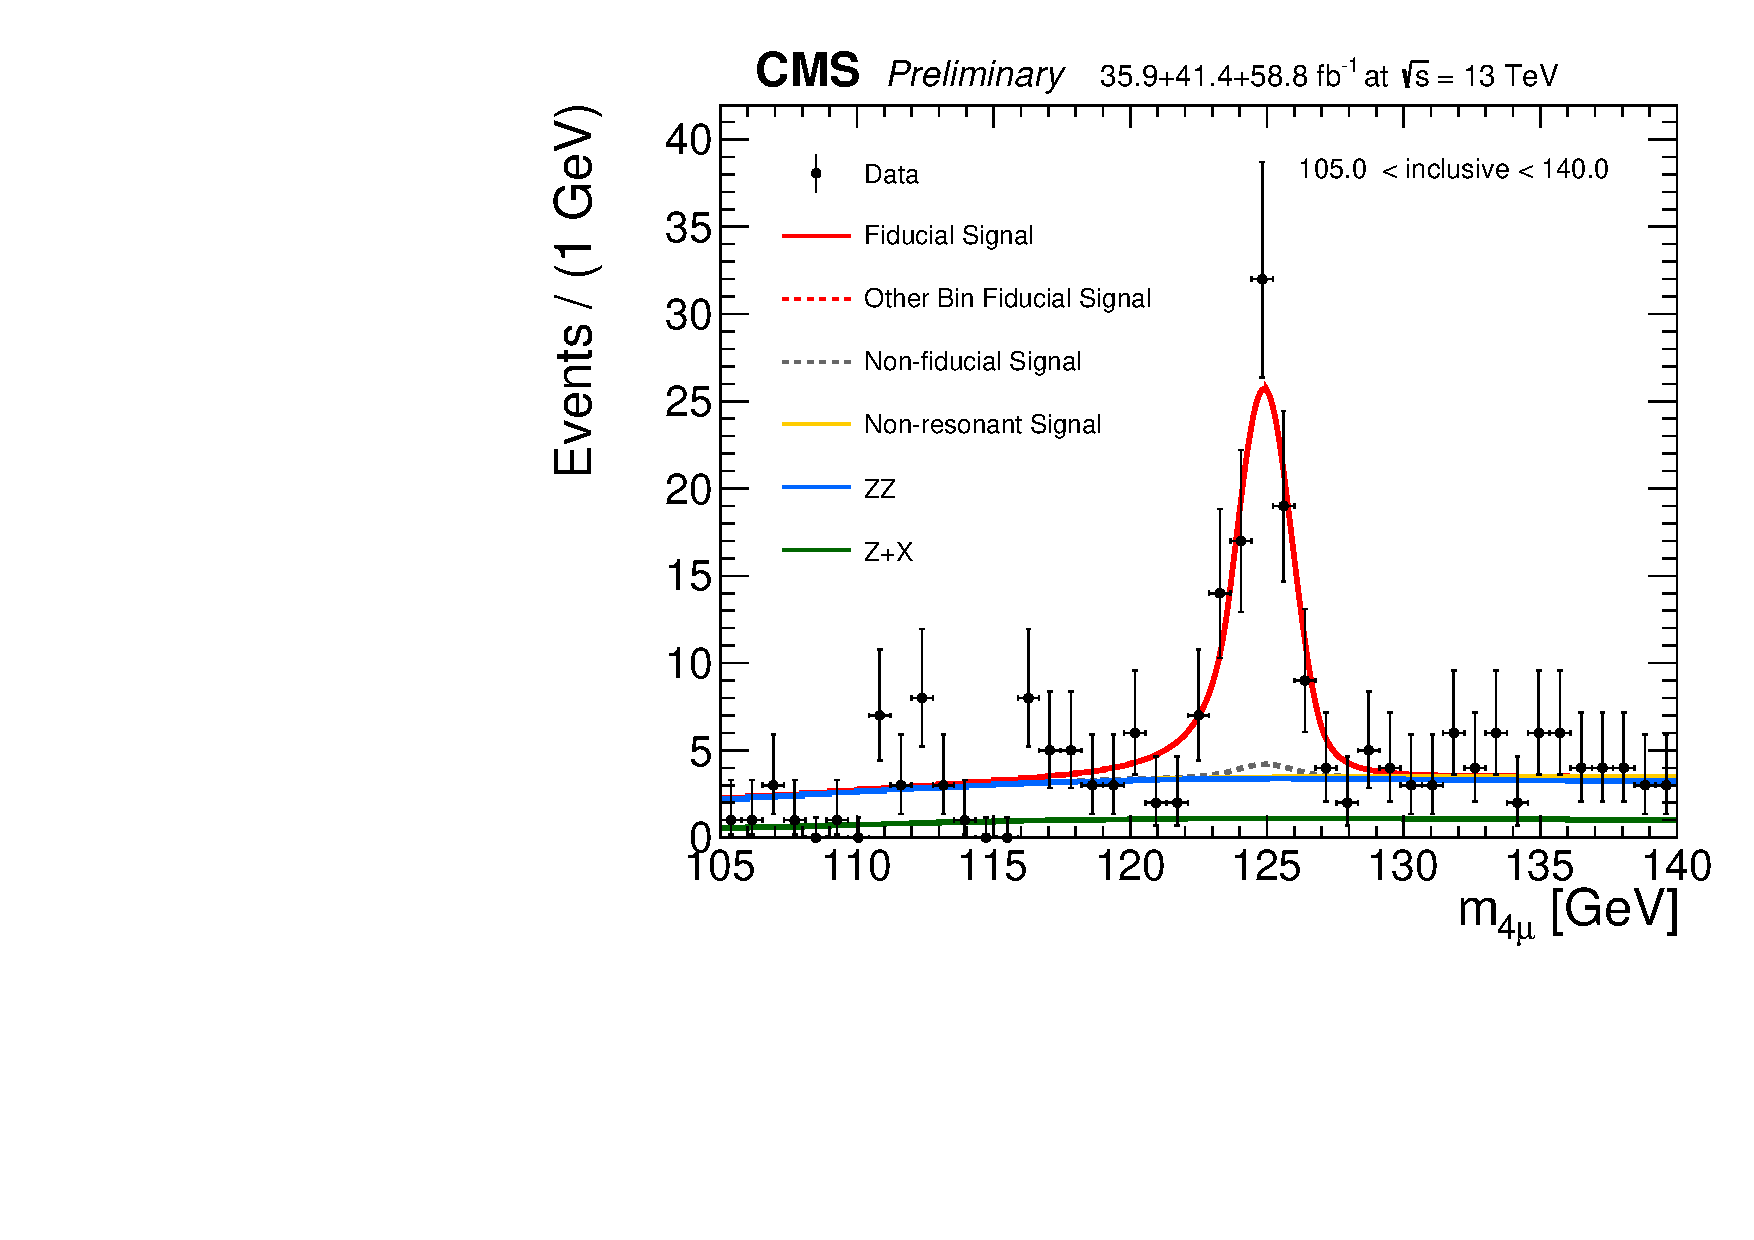
\includegraphics[width=0.45\linewidth]{Figures/results/fiducial/comb/unblind_Feb25/data_unfoldwith_SM_125_v3_mass4l_4mu_recobin0.pdf} \\
	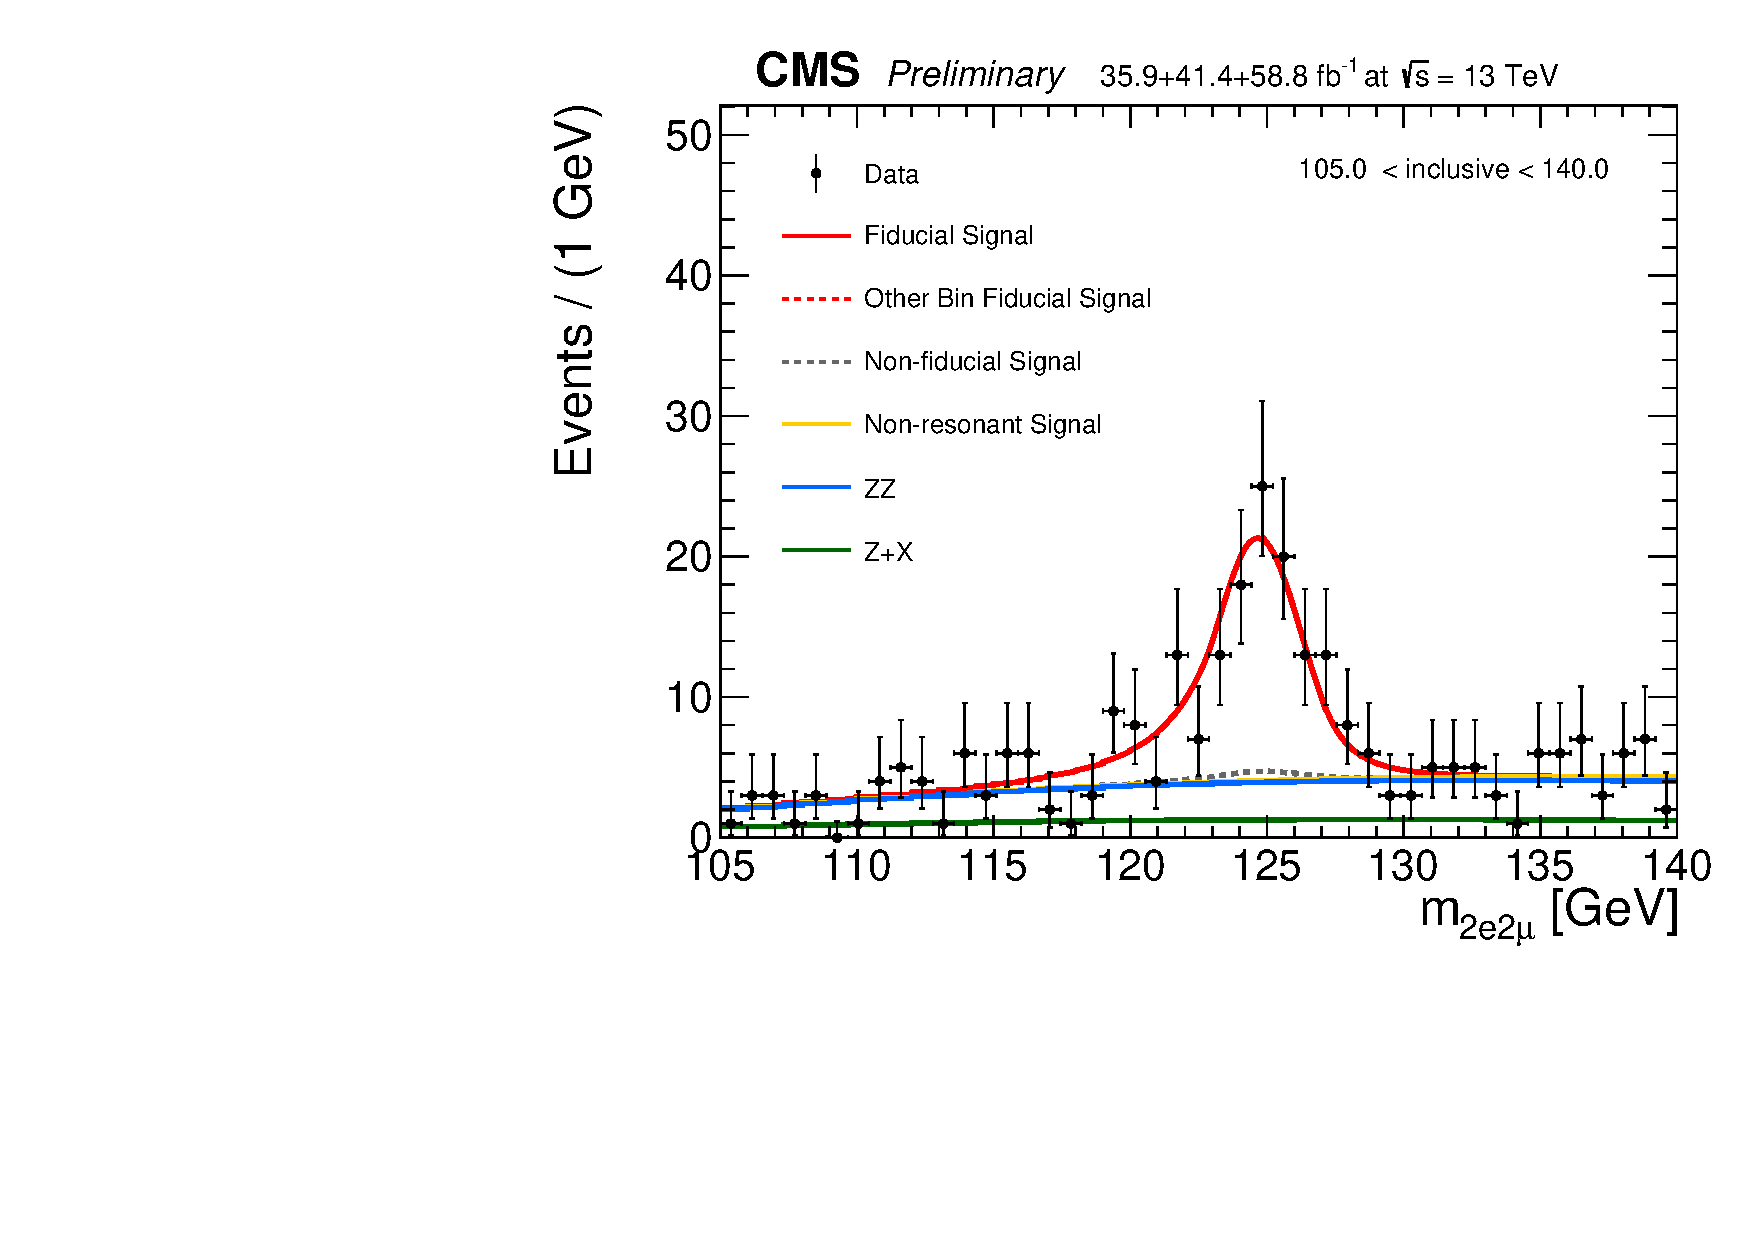
\includegraphics[width=0.45\linewidth]{Figures/results/fiducial/comb/unblind_Feb25/data_unfoldwith_SM_125_v3_mass4l_2e2mu_recobin0.pdf} 
	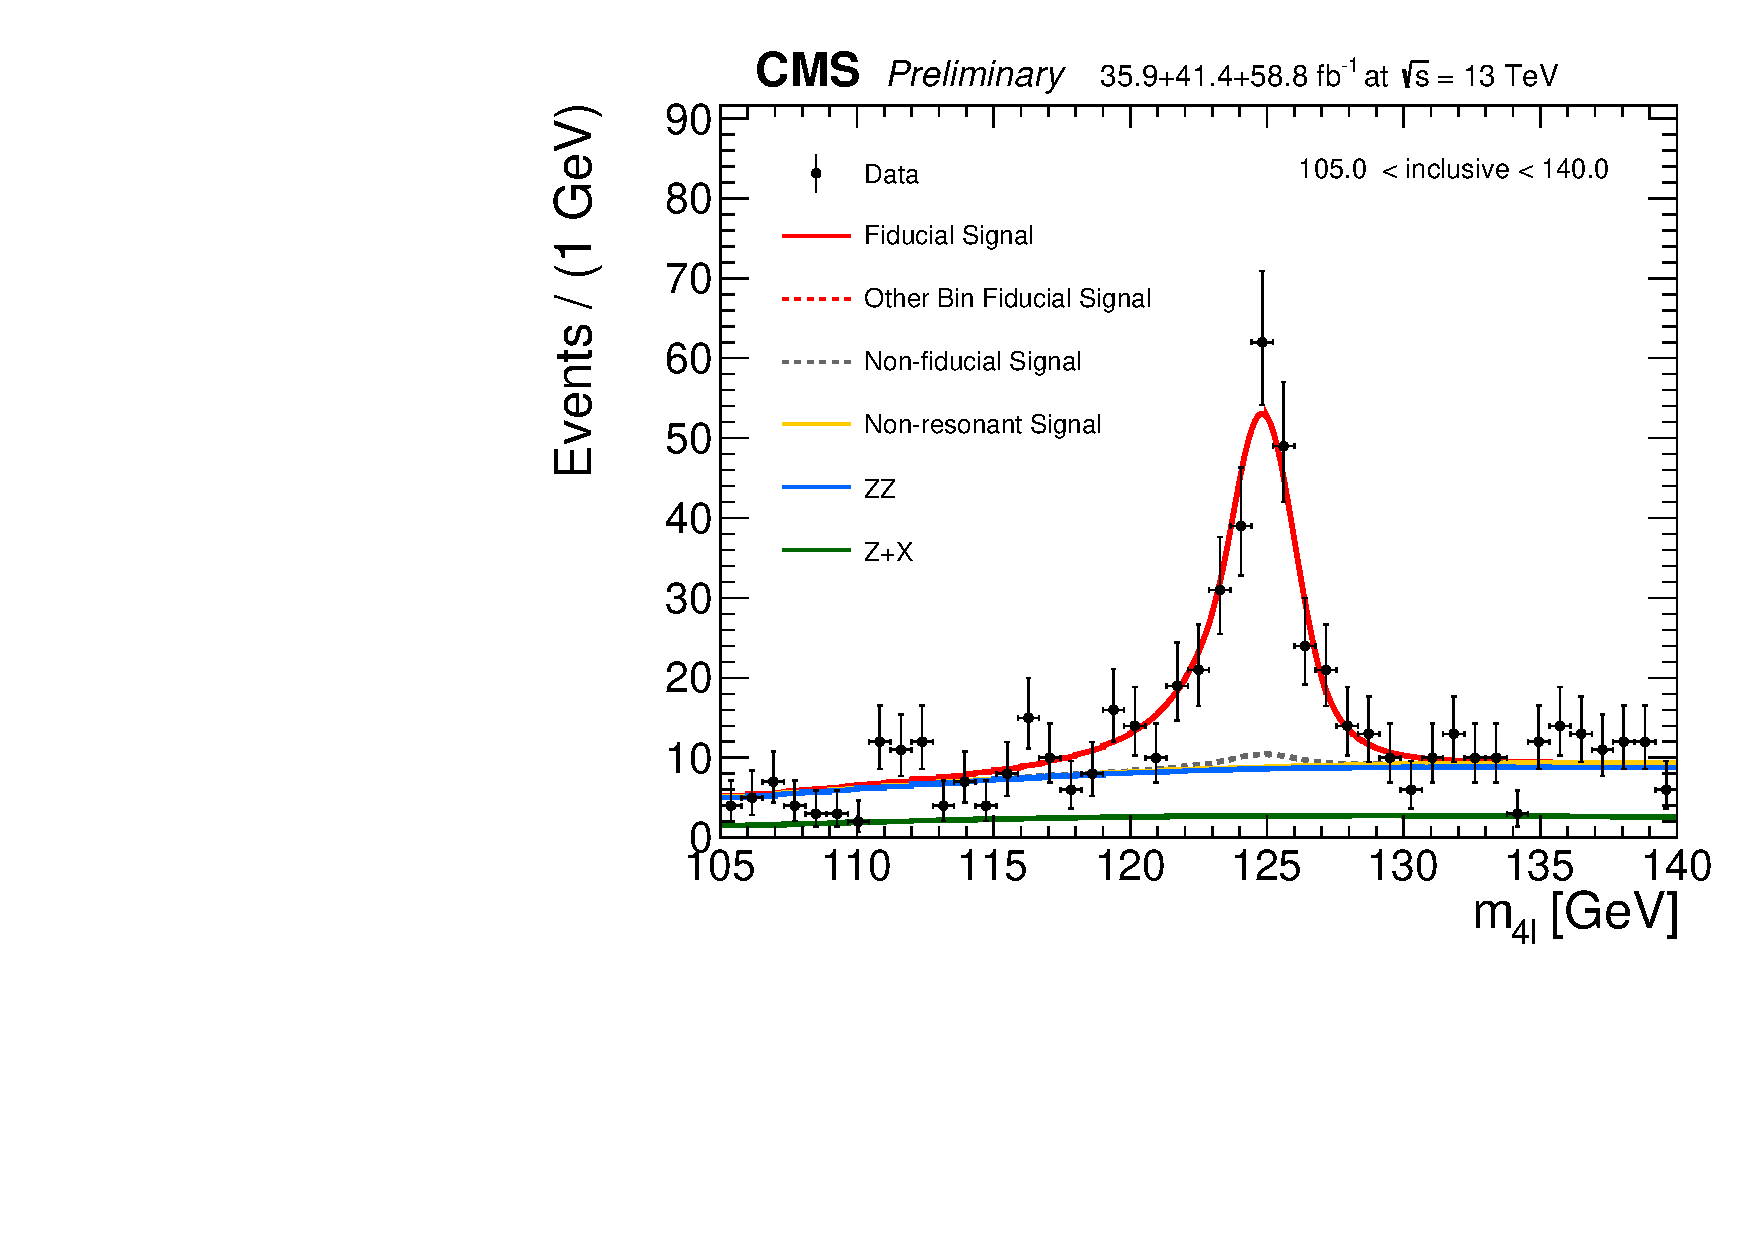
\includegraphics[width=0.45\linewidth]{Figures/results/fiducial/comb/unblind_Feb25/data_unfoldwith_SM_125_v3_mass4l_4l_recobin0.pdf} 
	\caption{Result of simultaneous fit for the integrated fiducial cross section measurement in each final state. The results are shown for 2018 only. \label{fig:fiducialfit}}
\end{figure}

\begin{figure}[!h]
	\centering
	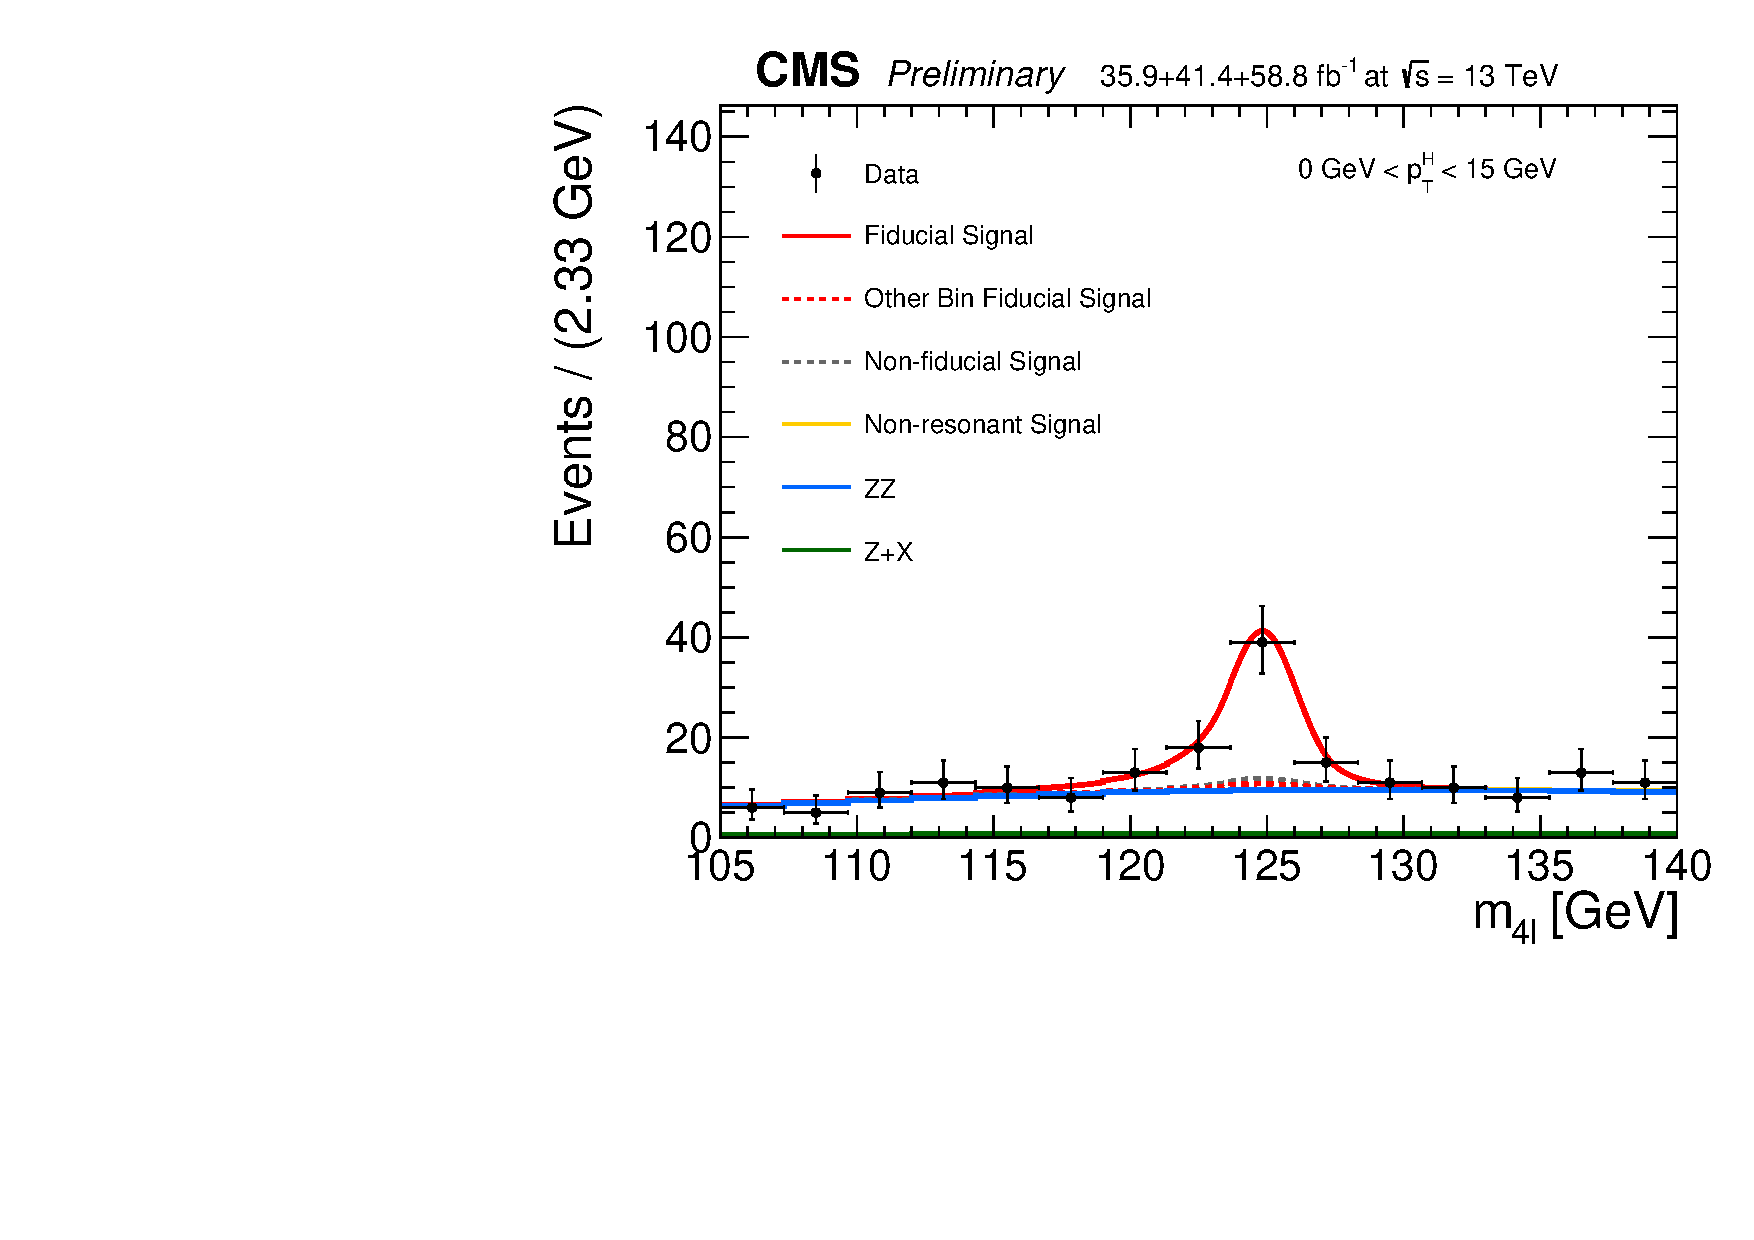
\includegraphics[width=0.32\linewidth]{Figures/results/fiducial/comb/unblind_Feb25/data_unfoldwith_SM_125_v3_pT4l_4l_recobin0.pdf}
	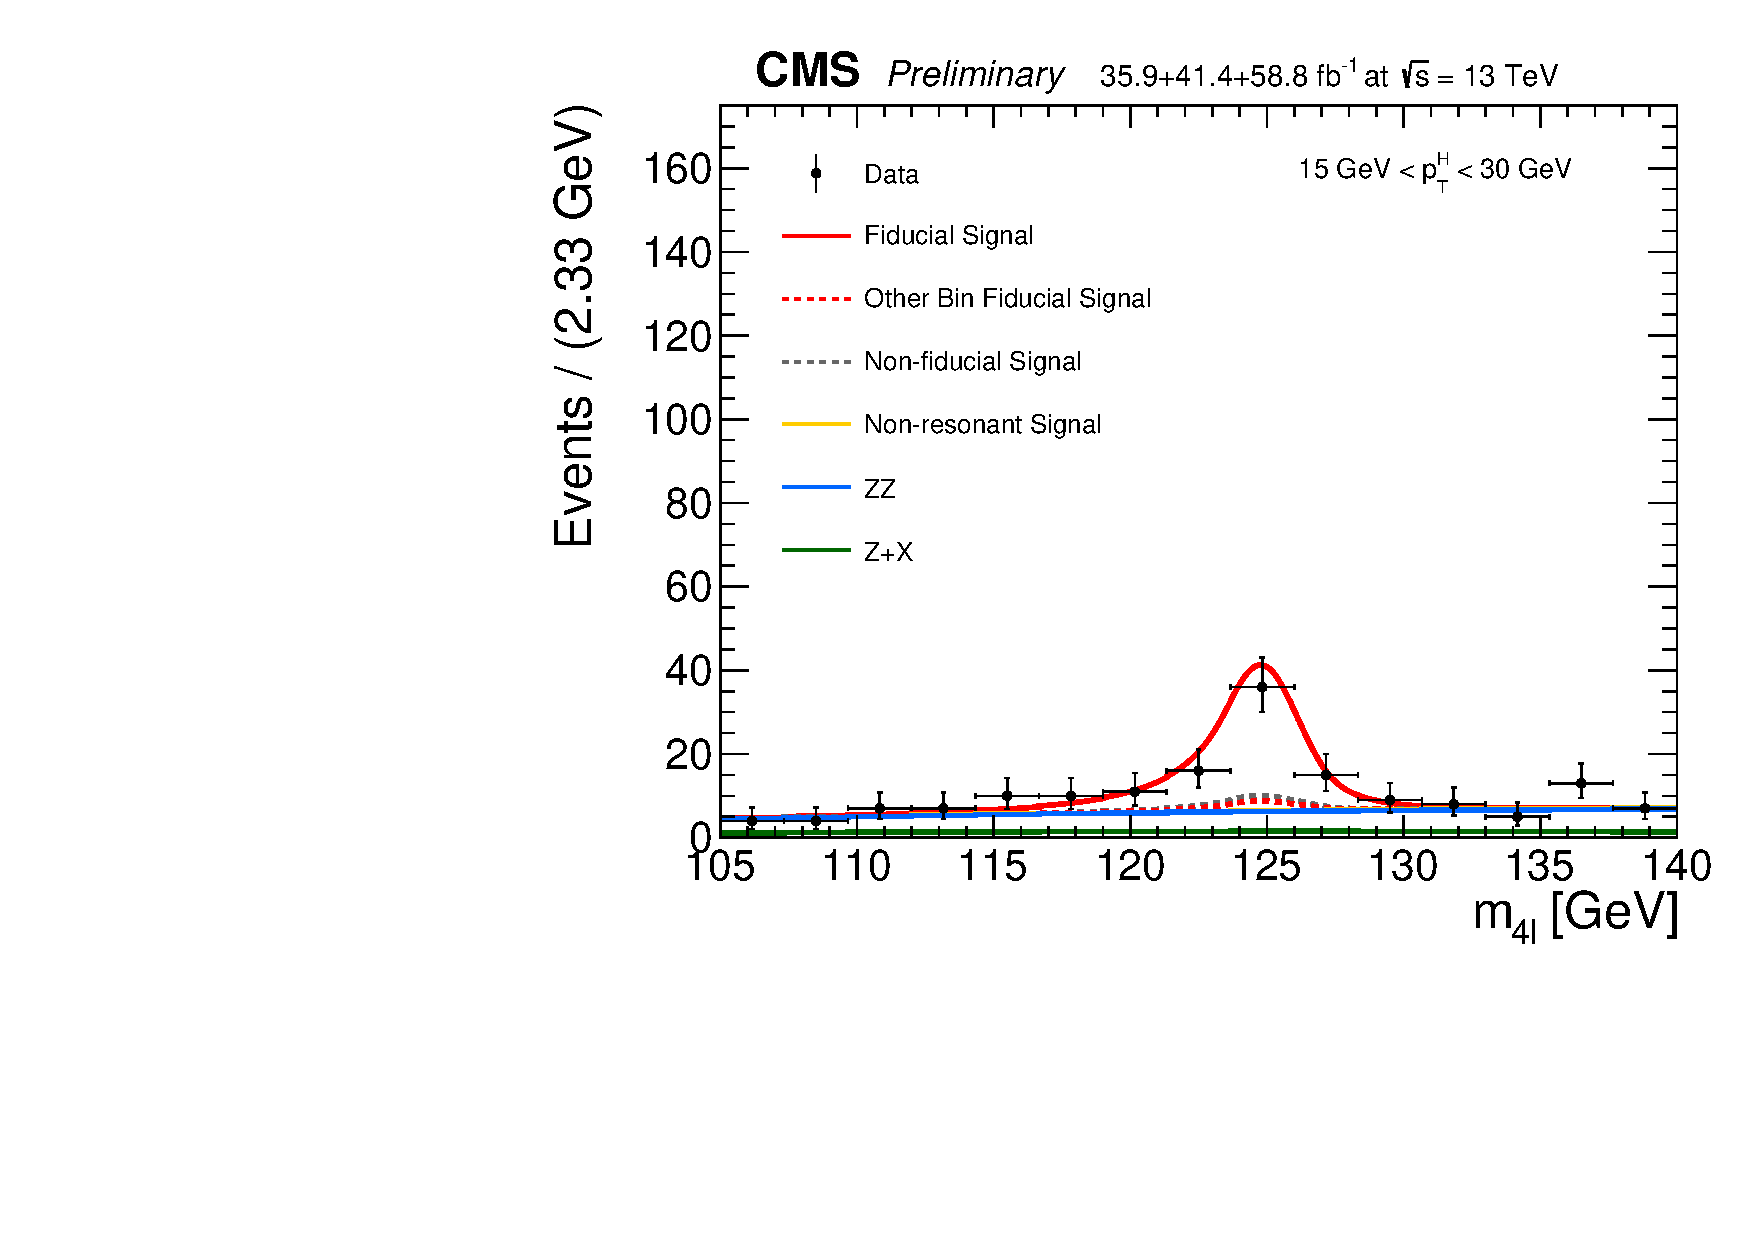
\includegraphics[width=0.32\linewidth]{Figures/results/fiducial/comb/unblind_Feb25/data_unfoldwith_SM_125_v3_pT4l_4l_recobin1.pdf}
	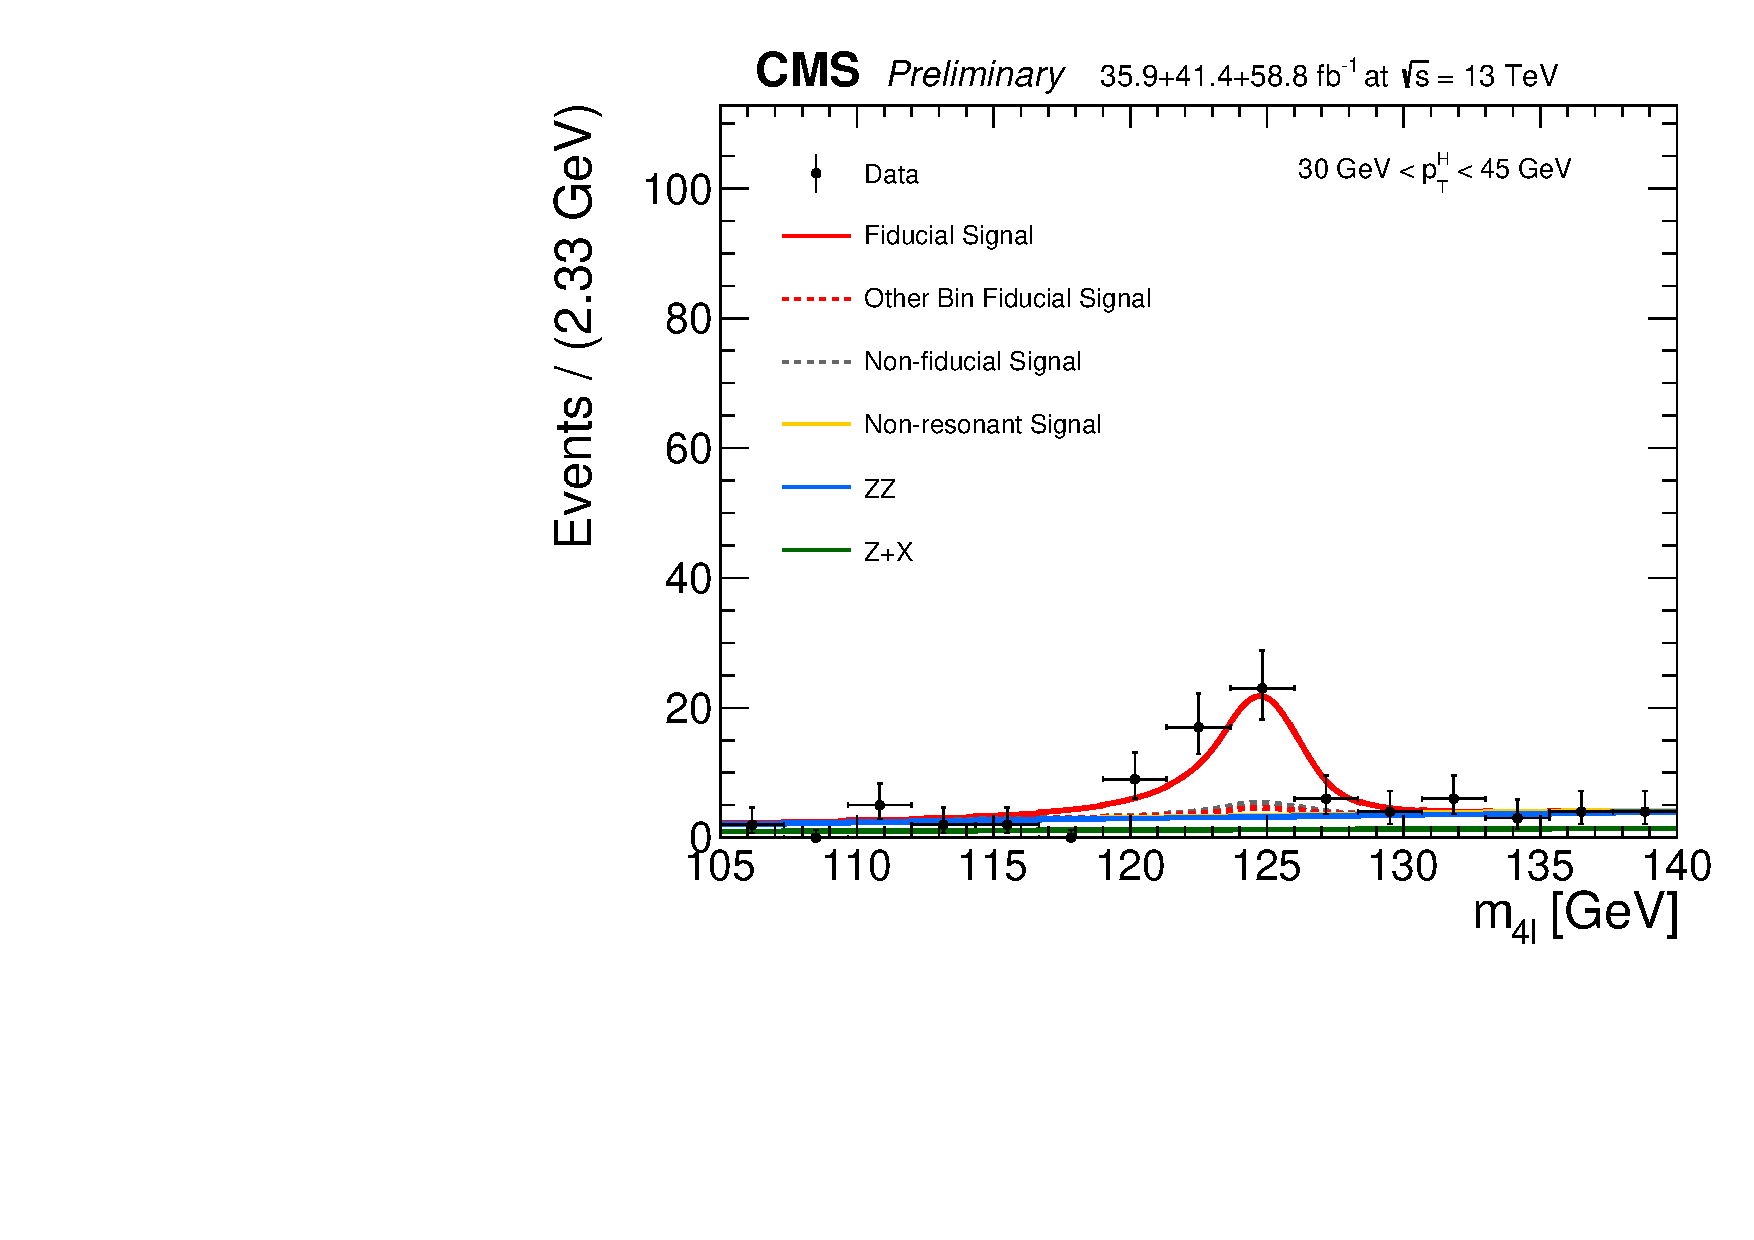
\includegraphics[width=0.32\linewidth]{Figures/results/fiducial/comb/unblind_Feb25/data_unfoldwith_SM_125_v3_pT4l_4l_recobin2.pdf}\\
	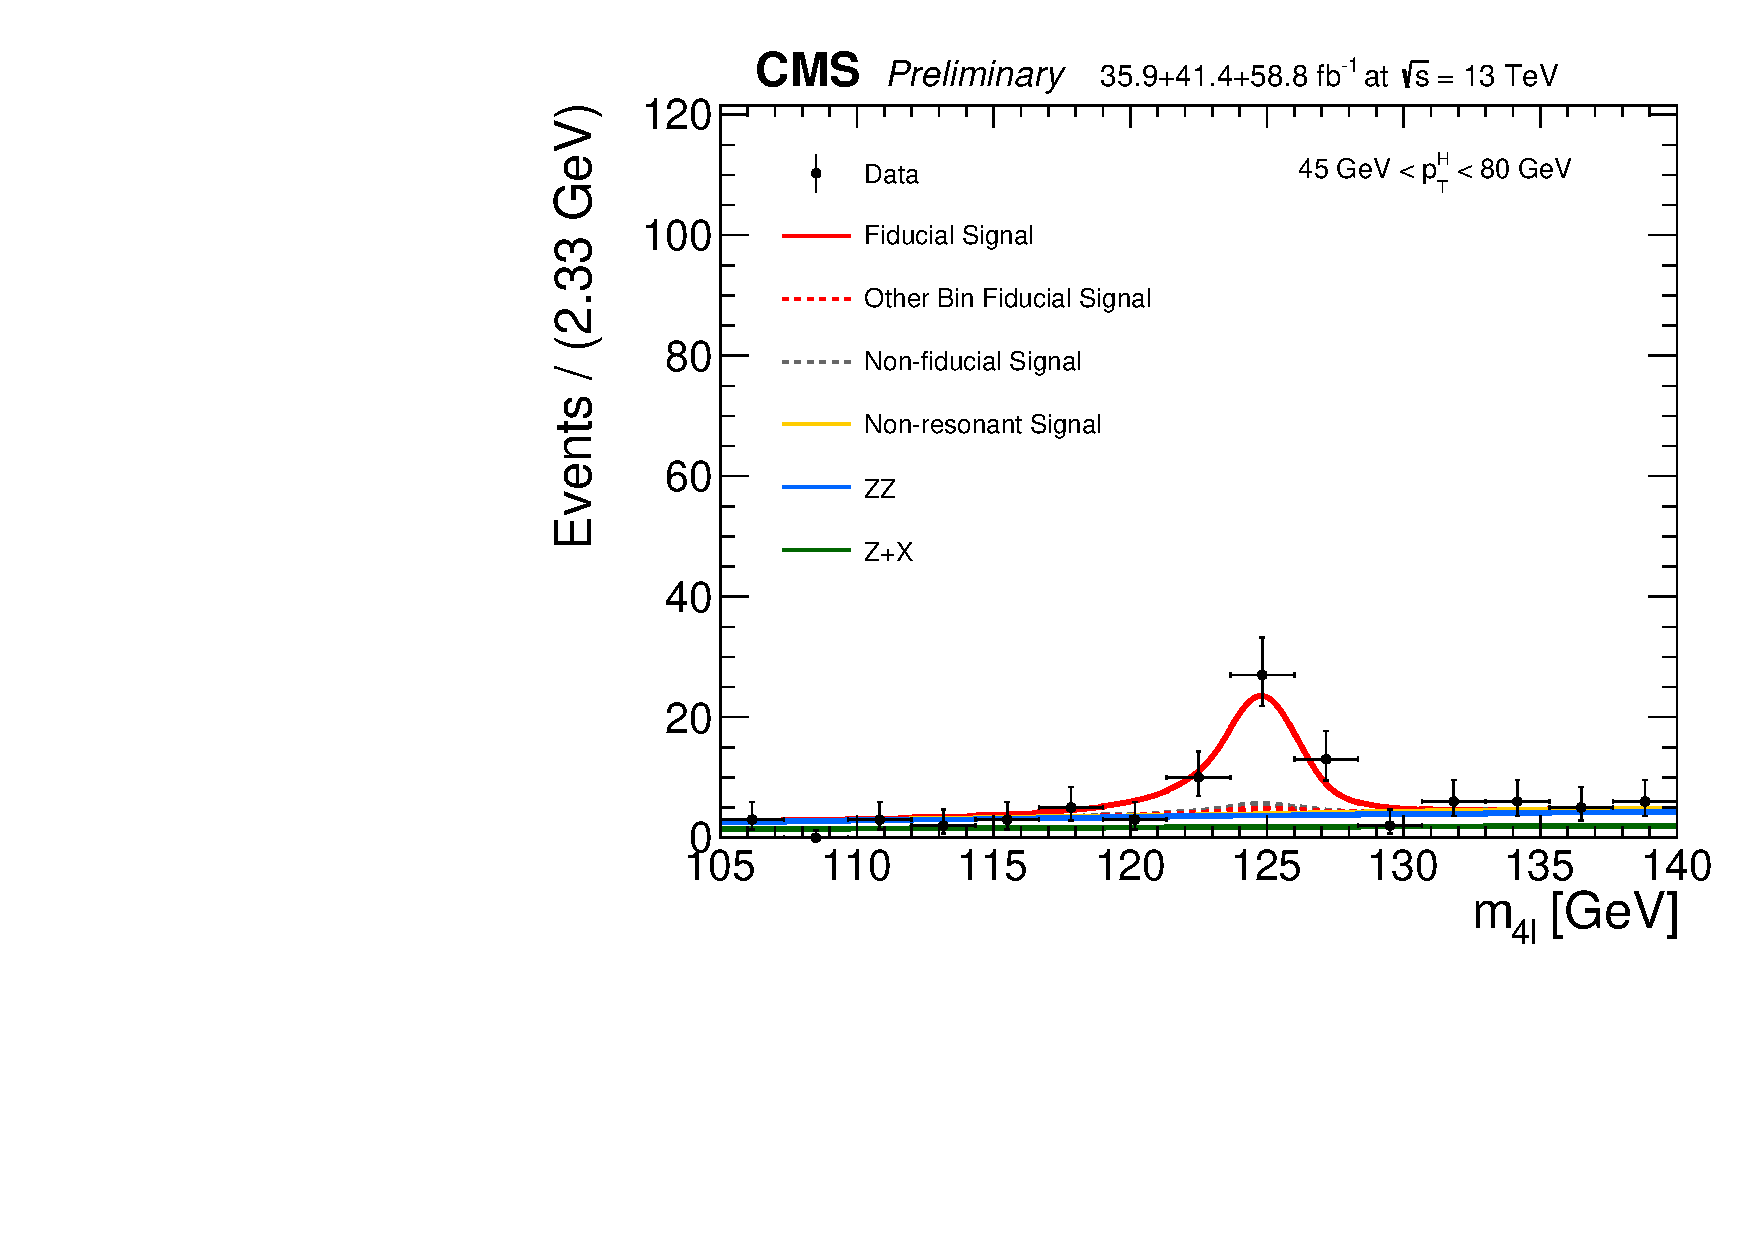
\includegraphics[width=0.32\linewidth]{Figures/results/fiducial/comb/unblind_Feb25/data_unfoldwith_SM_125_v3_pT4l_4l_recobin3.pdf}
	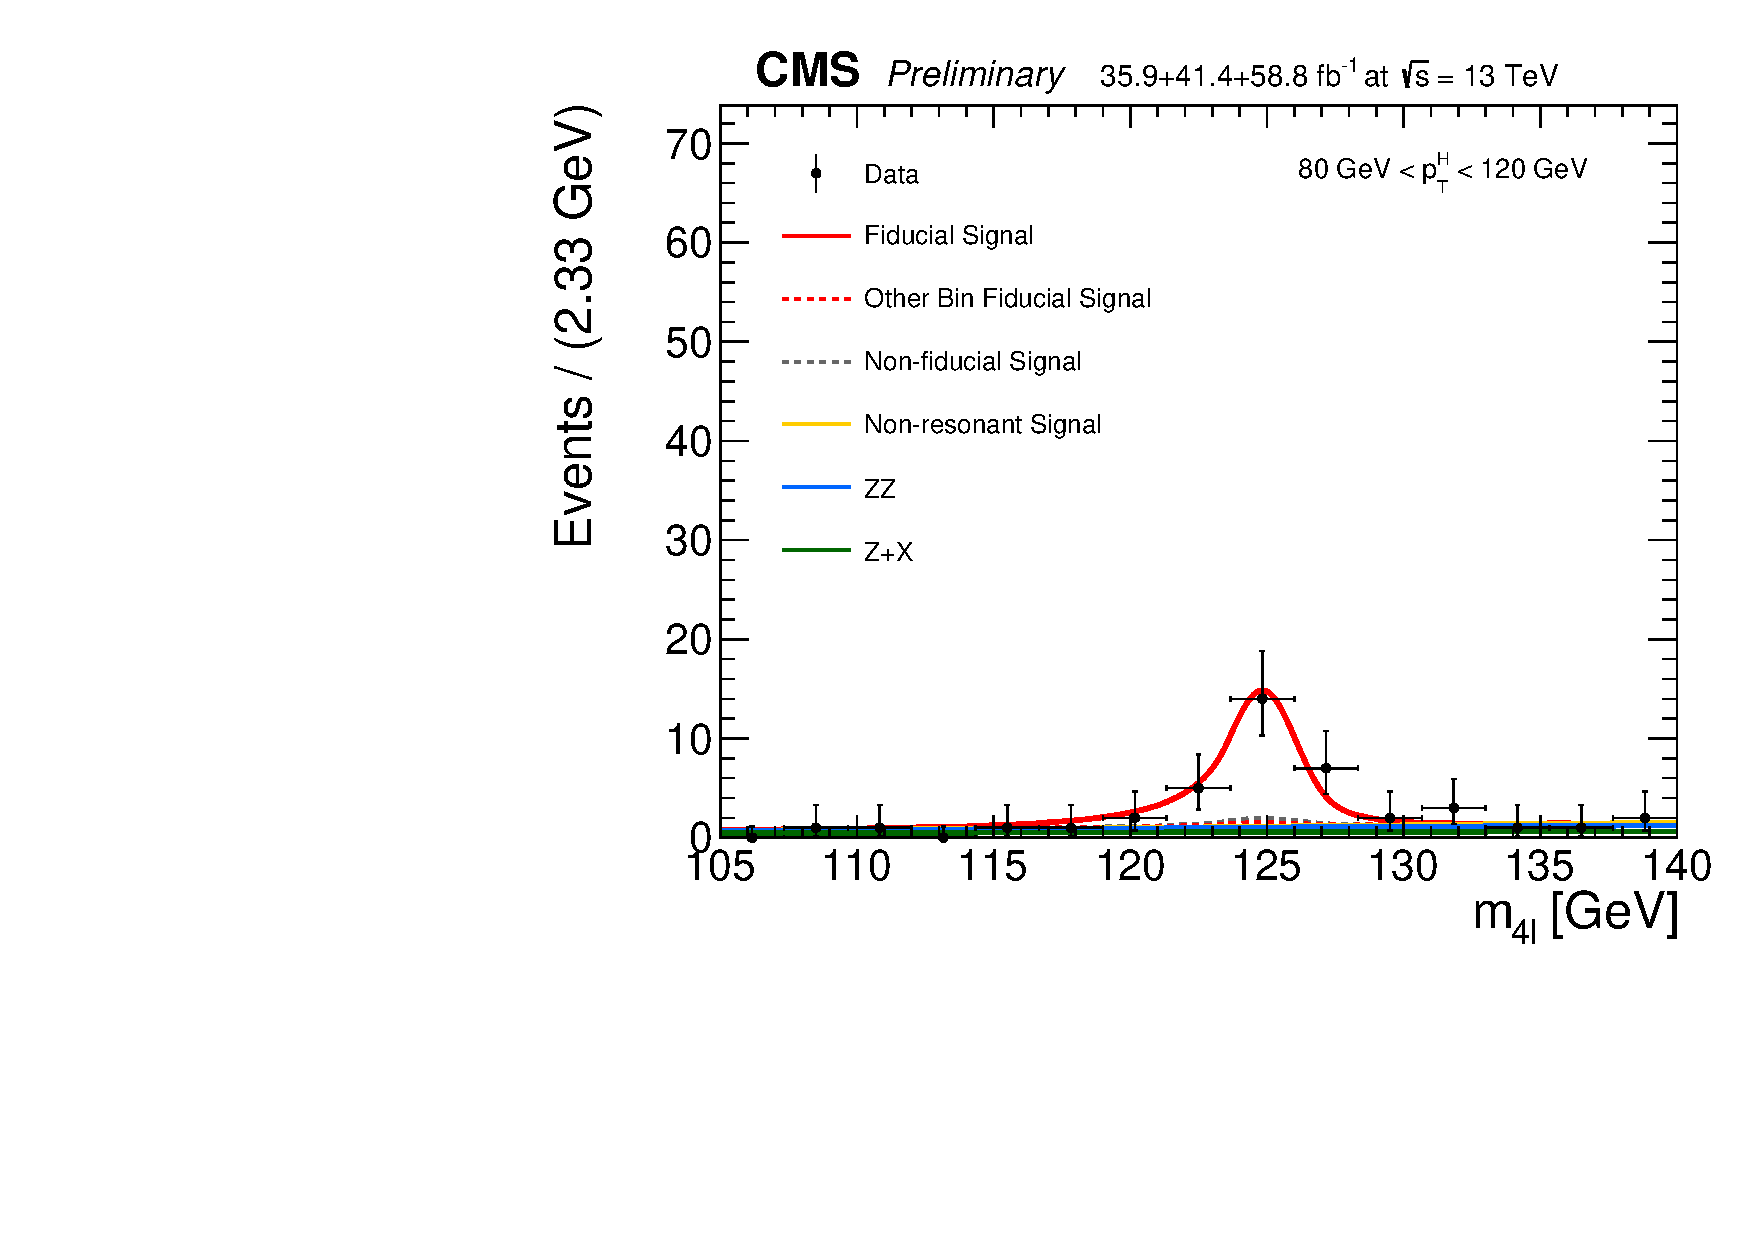
\includegraphics[width=0.32\linewidth]{Figures/results/fiducial/comb/unblind_Feb25/data_unfoldwith_SM_125_v3_pT4l_4l_recobin4.pdf}
	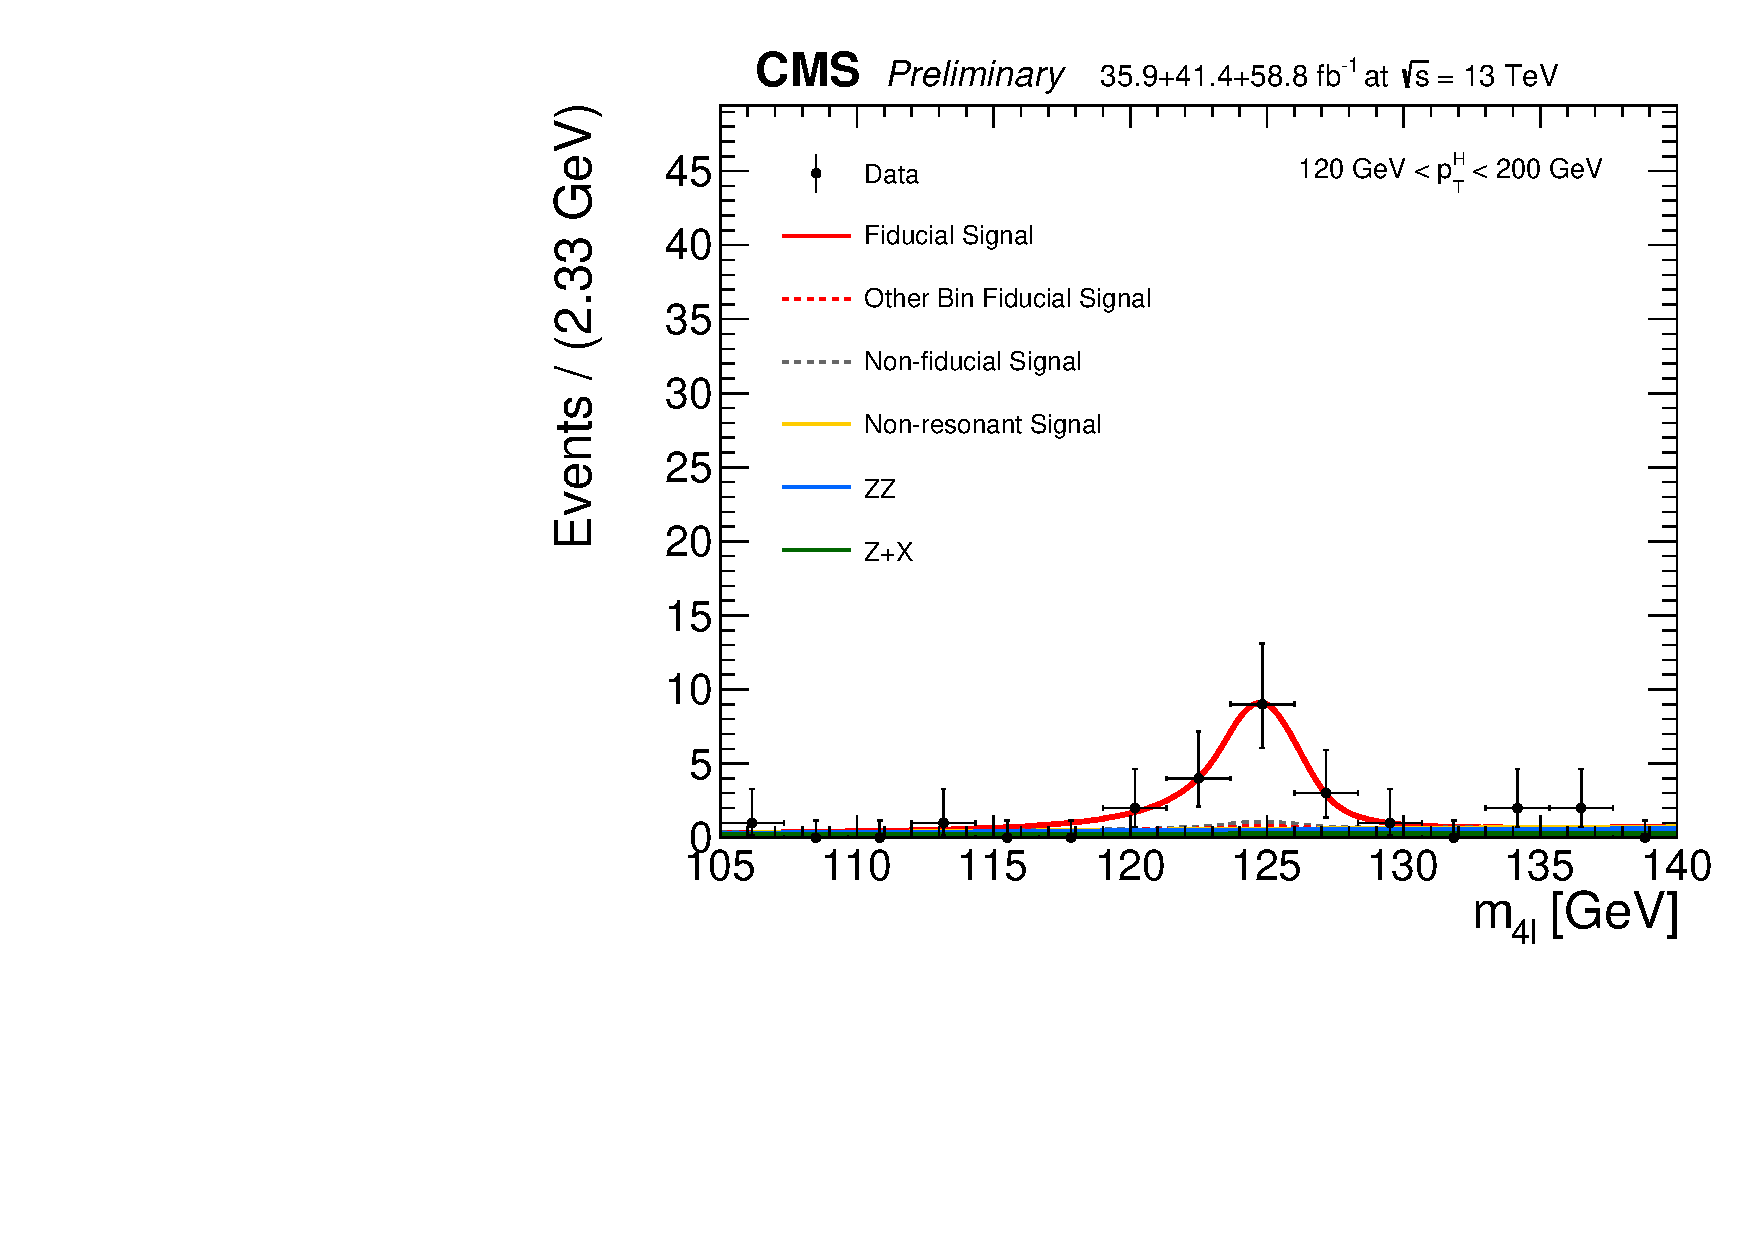
\includegraphics[width=0.32\linewidth]{Figures/results/fiducial/comb/unblind_Feb25/data_unfoldwith_SM_125_v3_pT4l_4l_recobin5.pdf} \\
	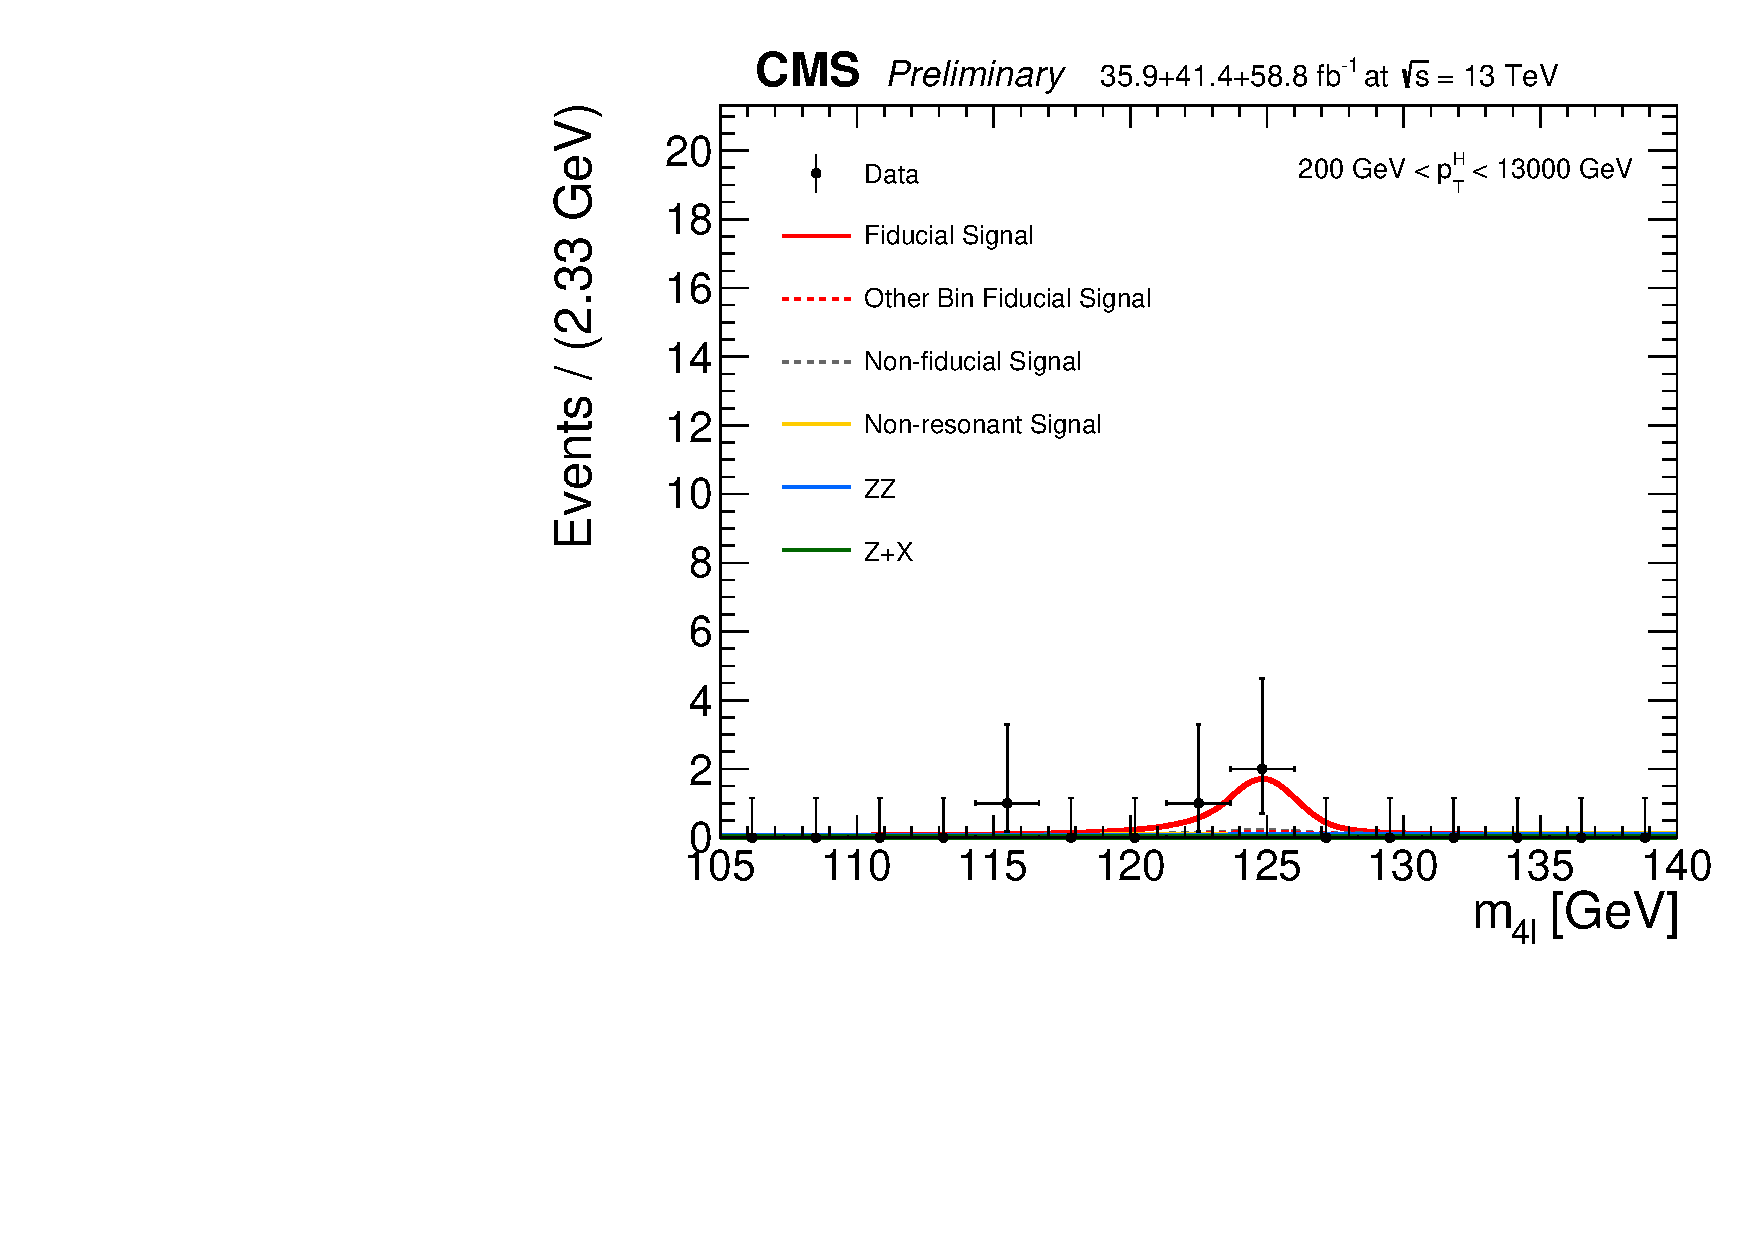
\includegraphics[width=0.32\linewidth]{Figures/results/fiducial/comb/unblind_Feb25/data_unfoldwith_SM_125_v3_pT4l_4l_recobin6.pdf}
	\caption{Result of simultaneous fit for the differential fiducial cross section measurement for $\pt({\rm H})$ 
		in each differential bin. The combined 4$\ell$ final state is shown. The results are shown for 2018 only. \label{fig:differentialfitptH}}
\end{figure}

\begin{figure}[!h]
	\centering 
	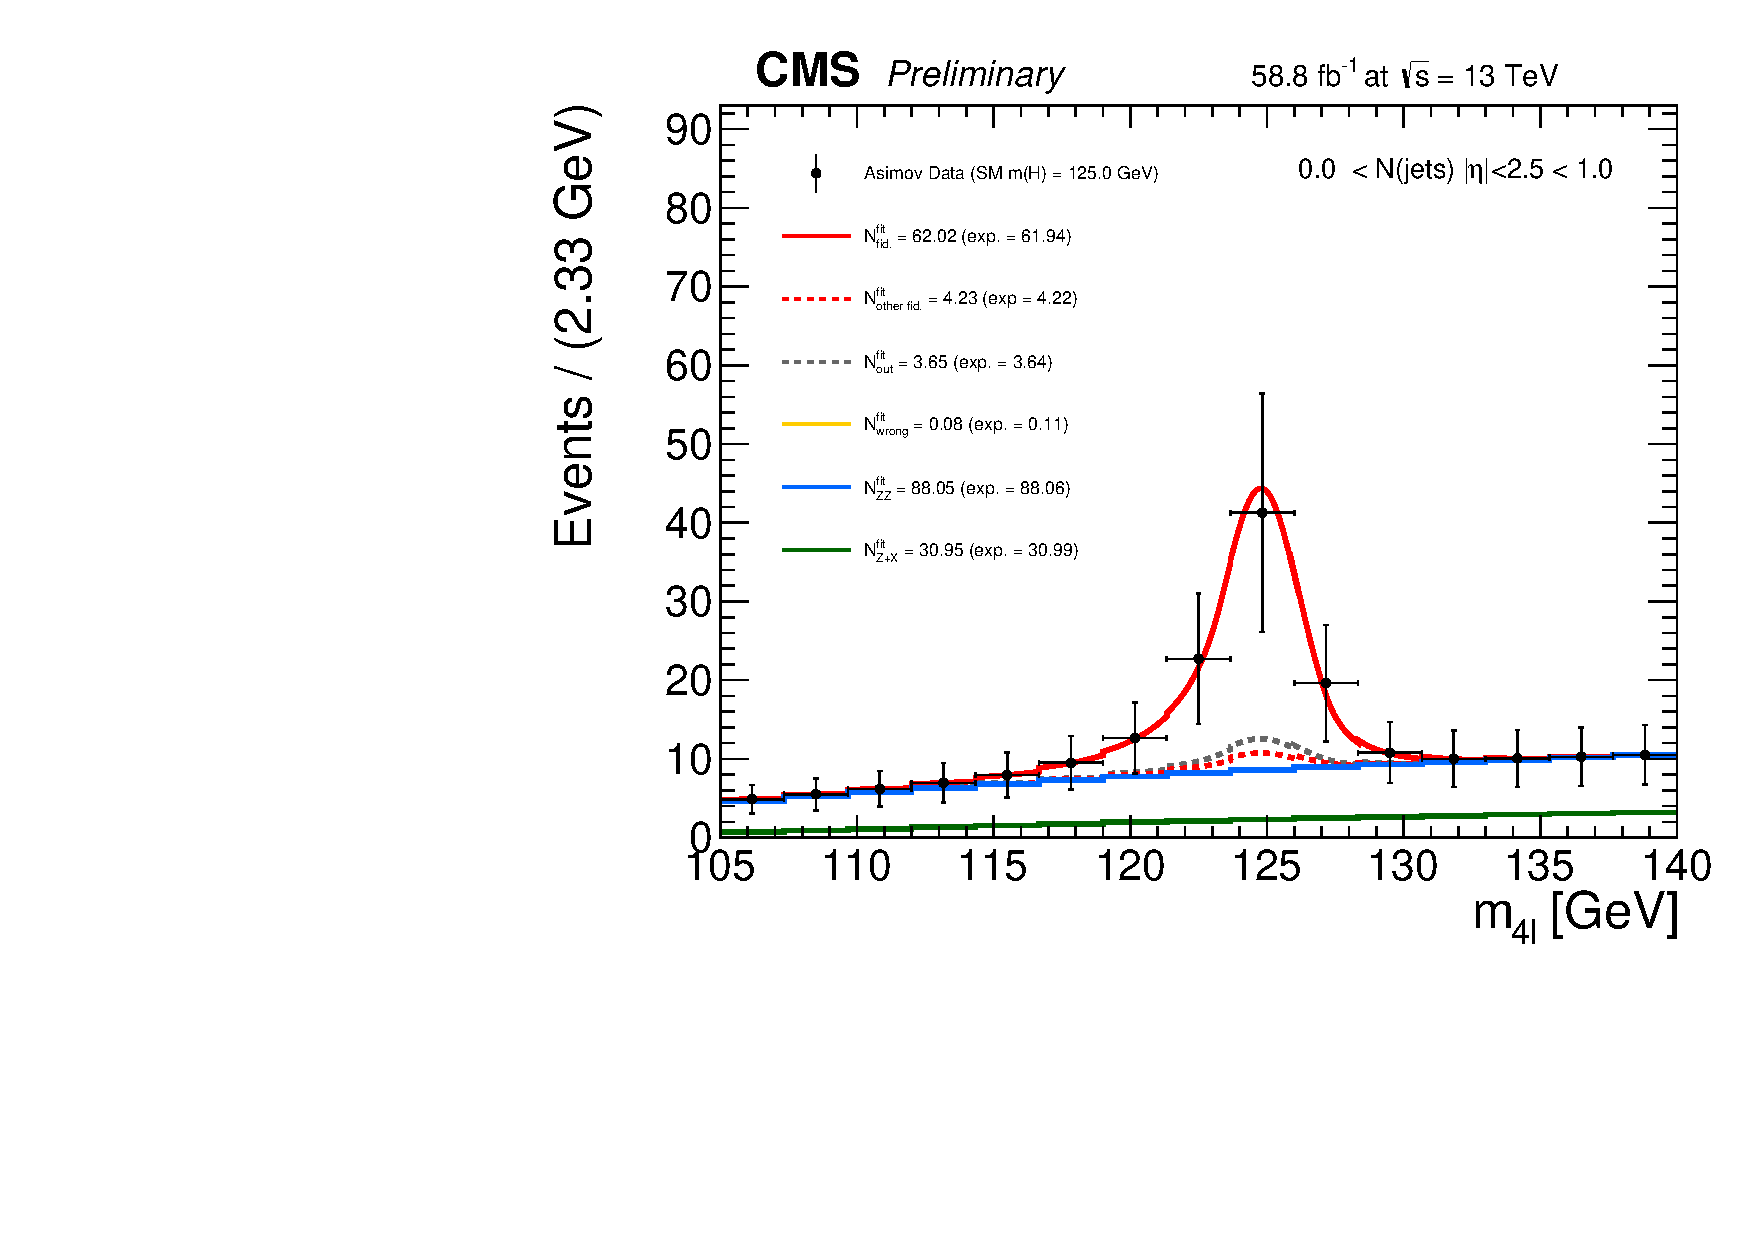
\includegraphics[width=0.32\linewidth]{Figures/results/fiducial/2018/asimovdata_SM_125_v2_unfoldwith_SM_125_v3_njets_pt30_eta2p5_4l_recobin0.pdf}
	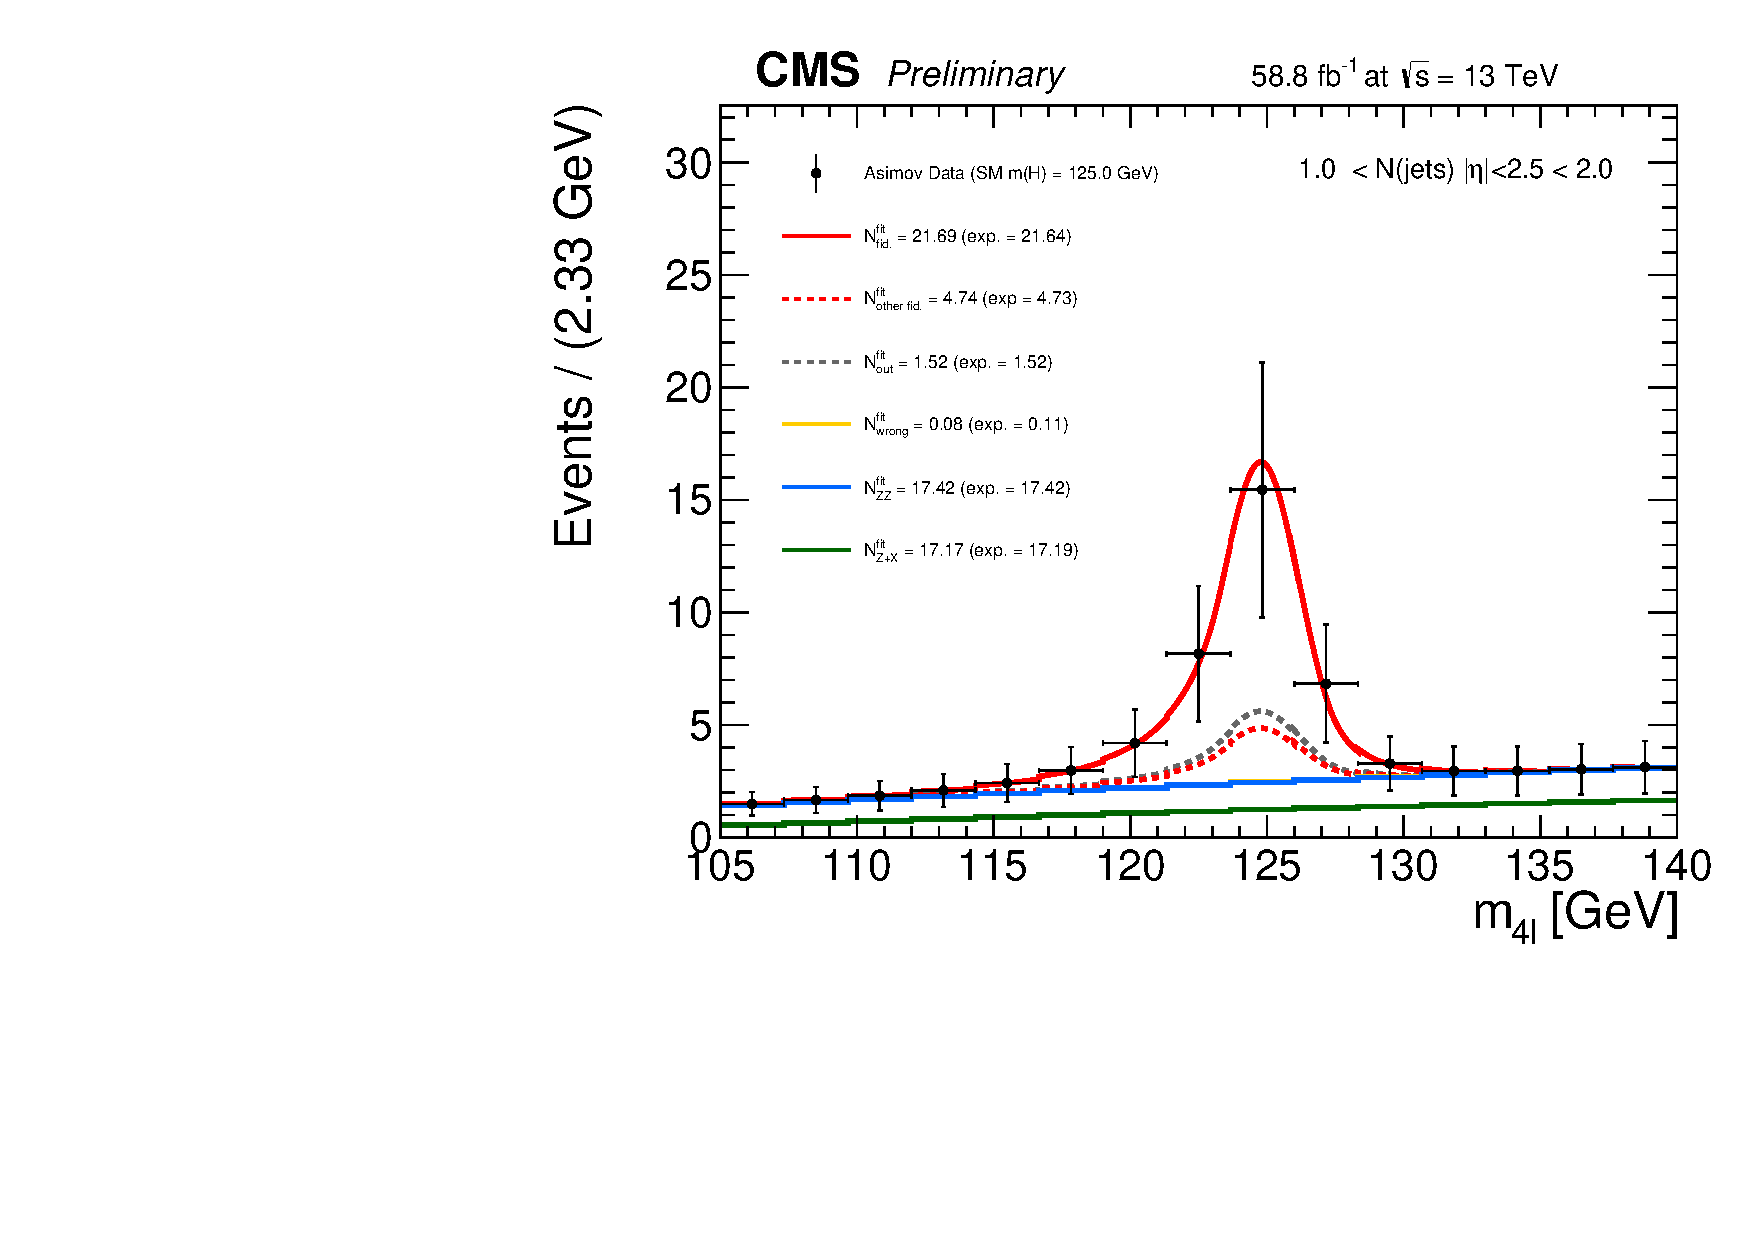
\includegraphics[width=0.32\linewidth]{Figures/results/fiducial/2018/asimovdata_SM_125_v2_unfoldwith_SM_125_v3_njets_pt30_eta2p5_4l_recobin1.pdf}
	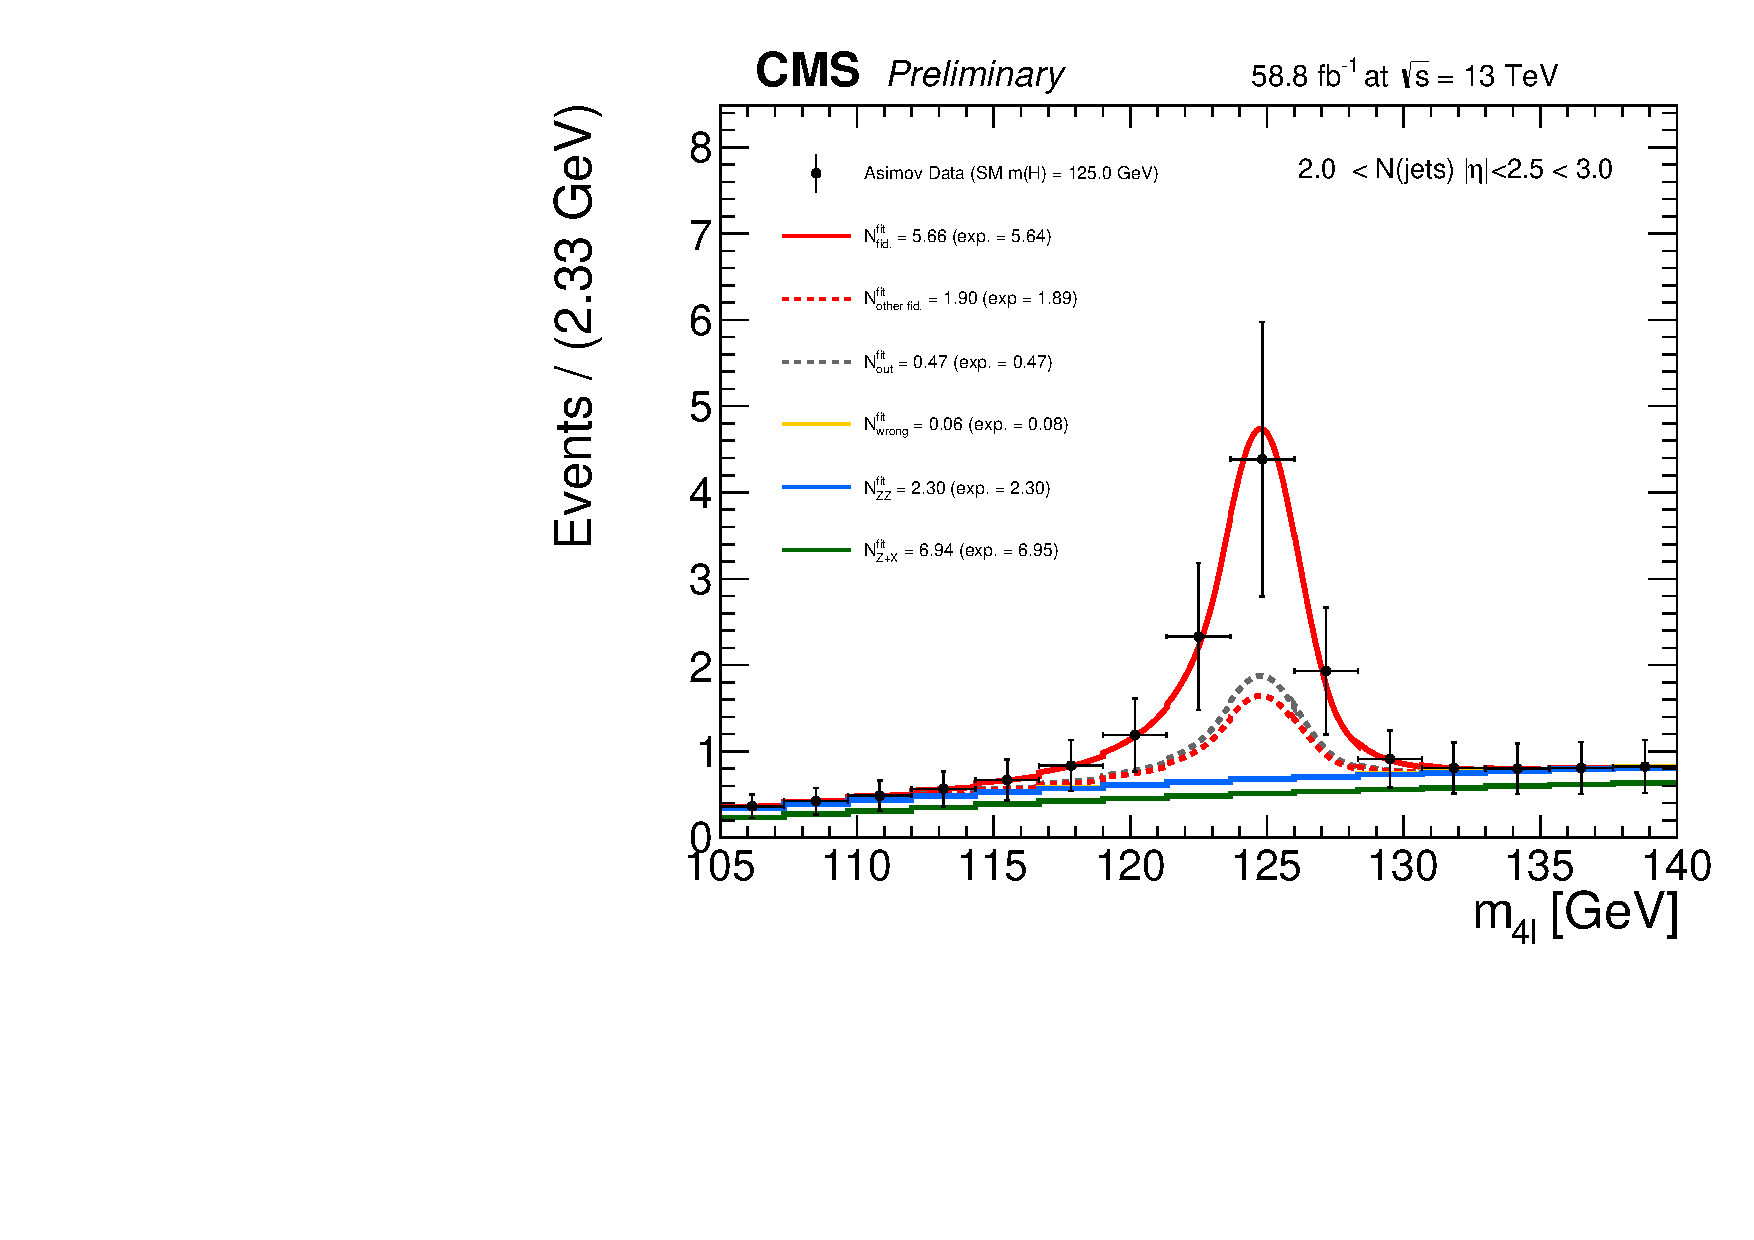
\includegraphics[width=0.32\linewidth]{Figures/results/fiducial/2018/asimovdata_SM_125_v2_unfoldwith_SM_125_v3_njets_pt30_eta2p5_4l_recobin2.pdf} \\
	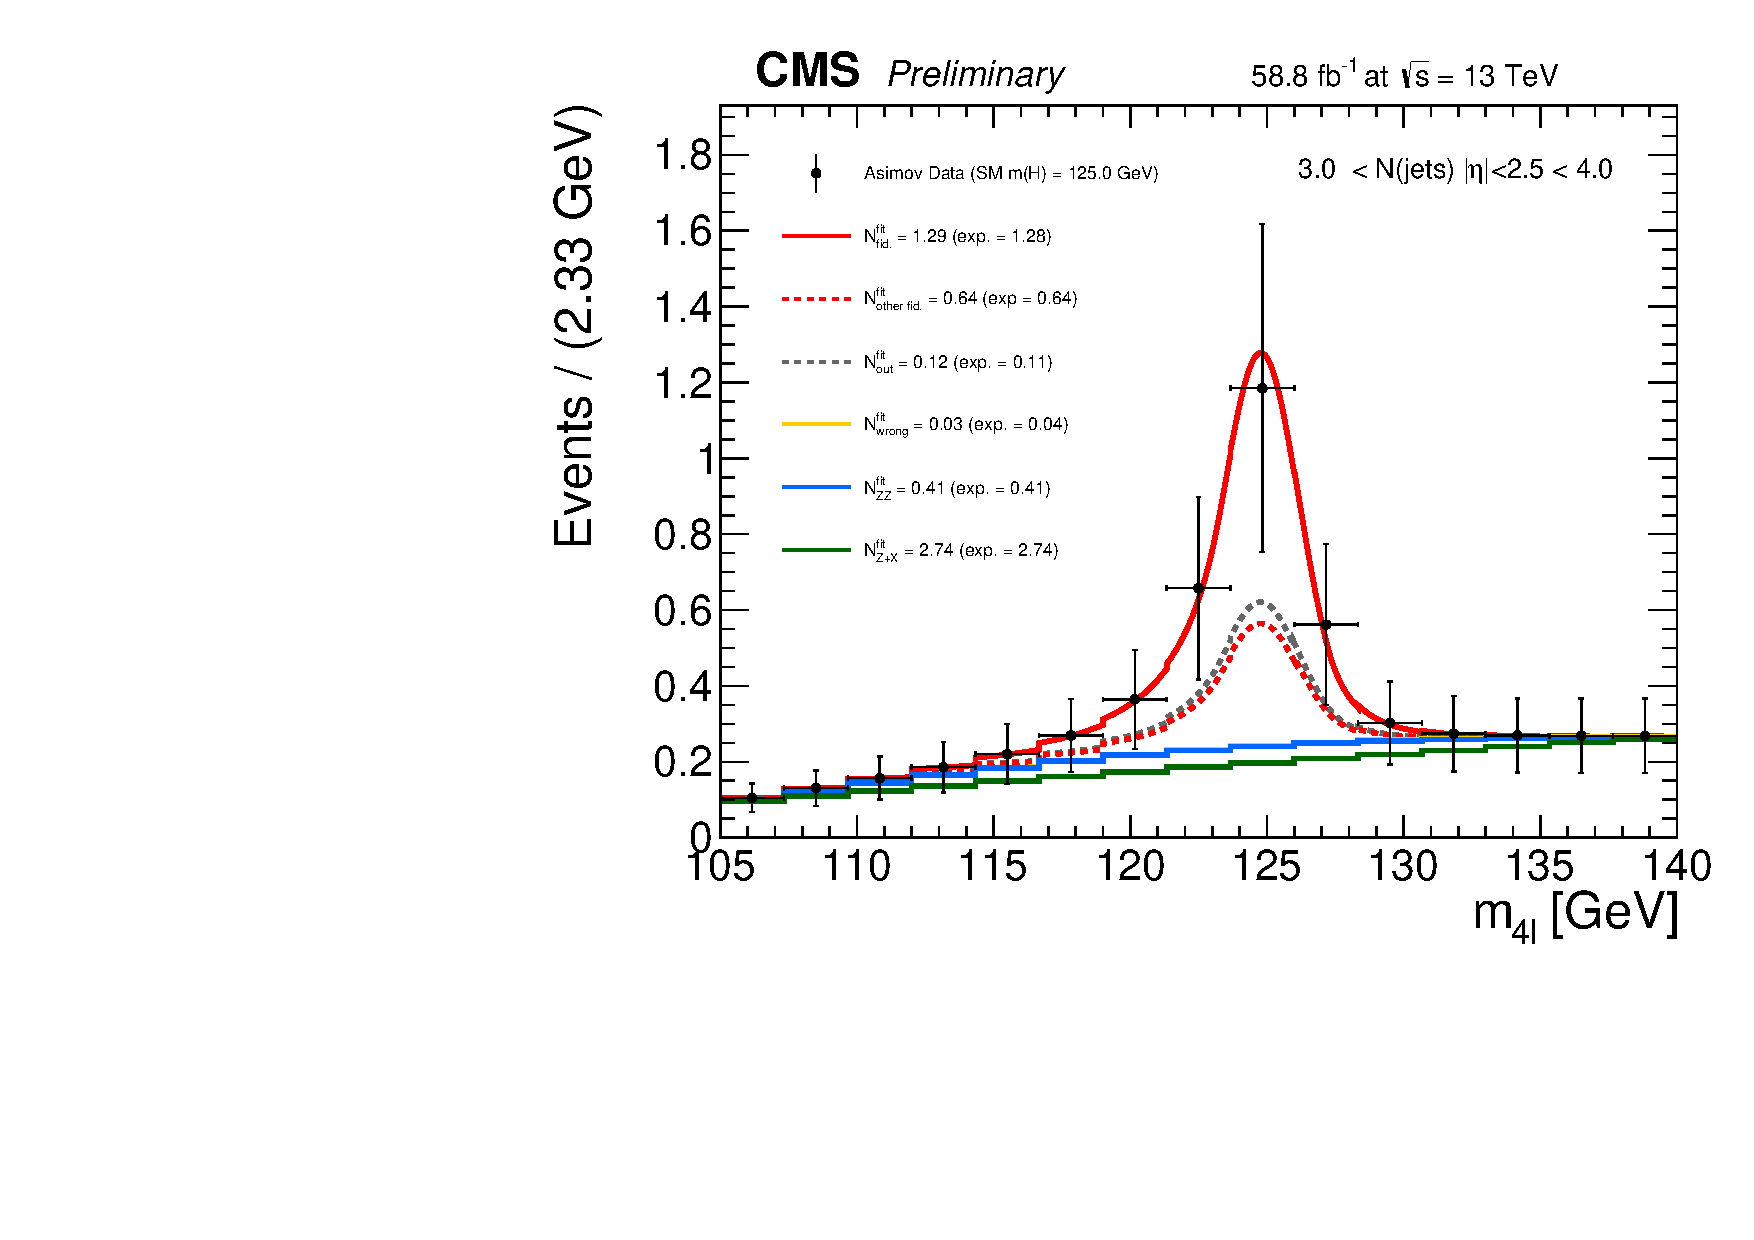
\includegraphics[width=0.32\linewidth]{Figures/results/fiducial/2018/asimovdata_SM_125_v2_unfoldwith_SM_125_v3_njets_pt30_eta2p5_4l_recobin3.pdf}
	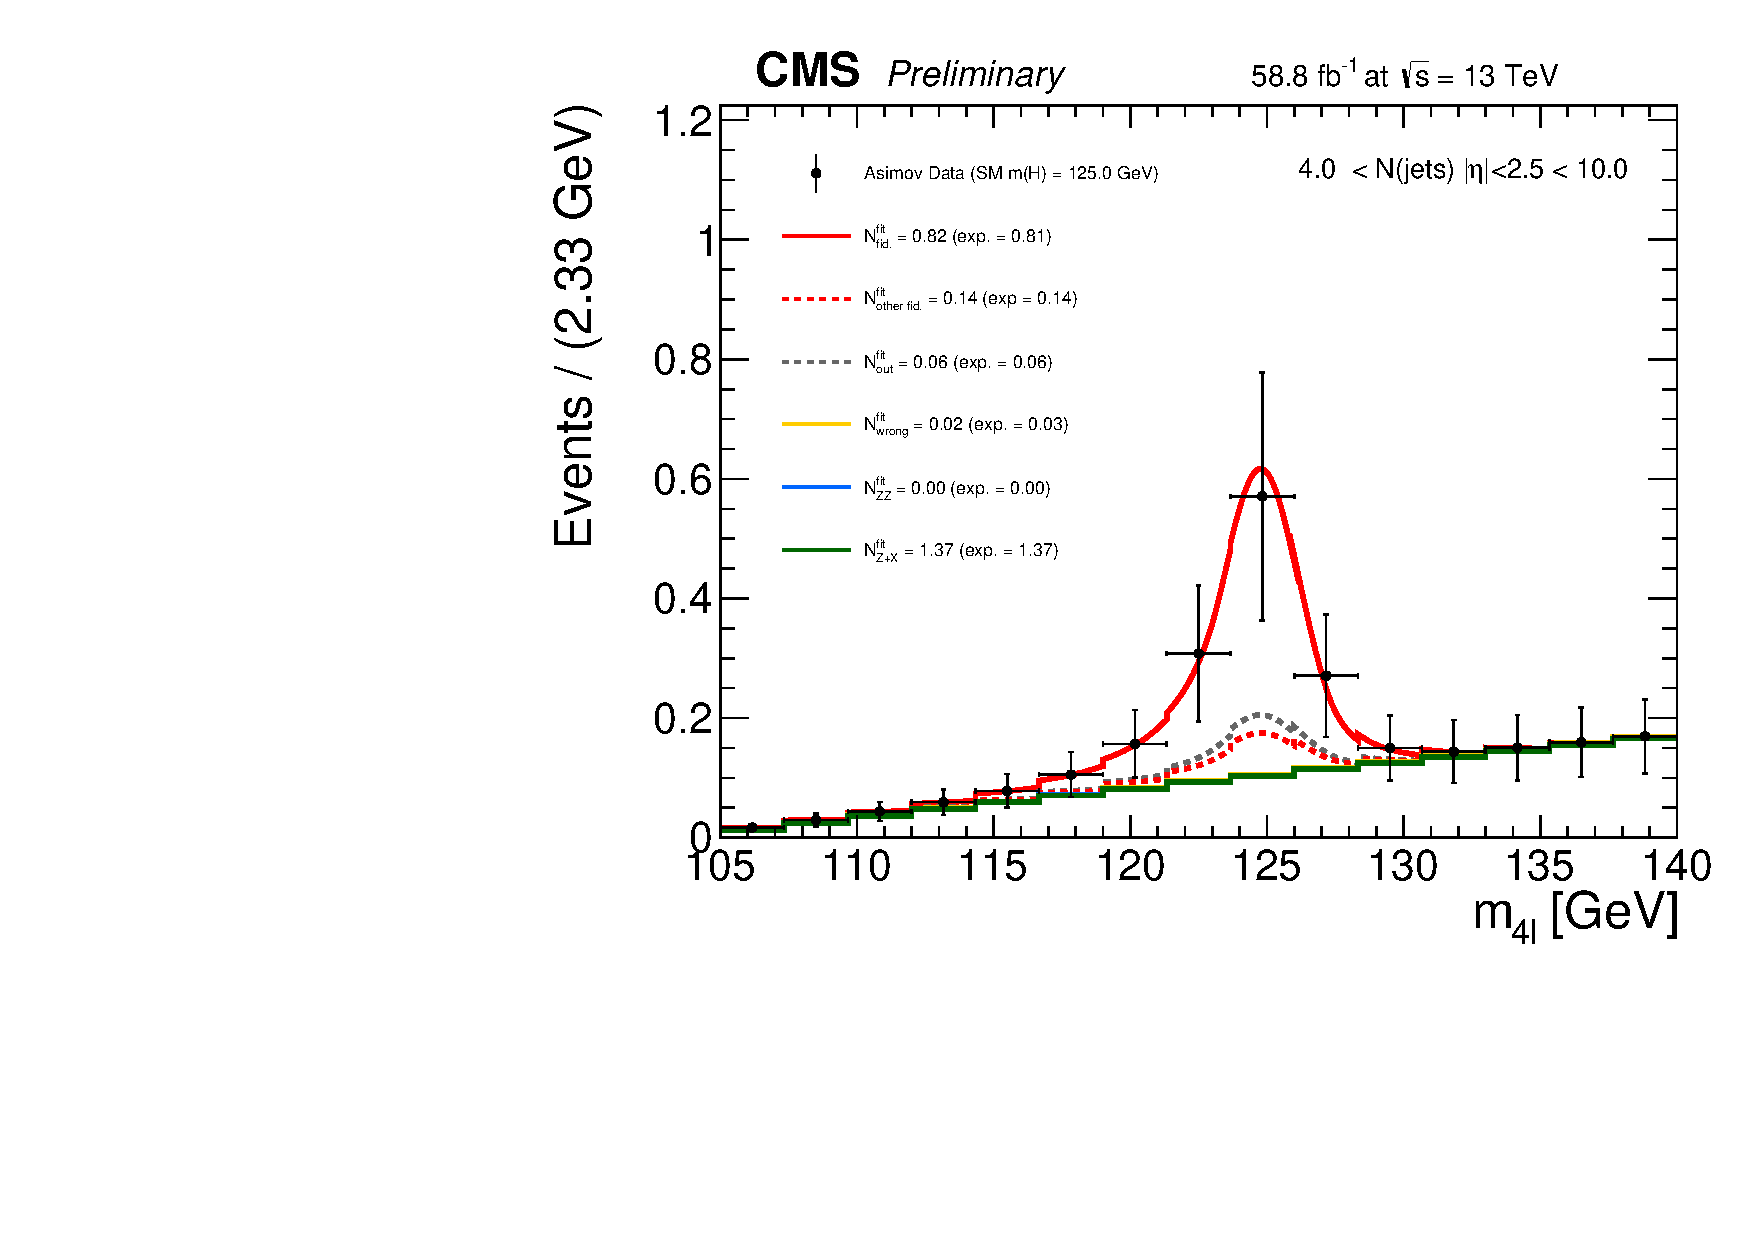
\includegraphics[width=0.32\linewidth]{Figures/results/fiducial/2018/asimovdata_SM_125_v2_unfoldwith_SM_125_v3_njets_pt30_eta2p5_4l_recobin4.pdf}
	\caption{Result of simultaneous fit for the differential fiducial cross section measurement for N(jets) 
		in each differential bin. The combined 4$\ell$ final state is shown. The results are shown for 2018 only. \label{fig:differentialfitNjets}}
\end{figure}

\begin{figure}[!h]
	\centering
	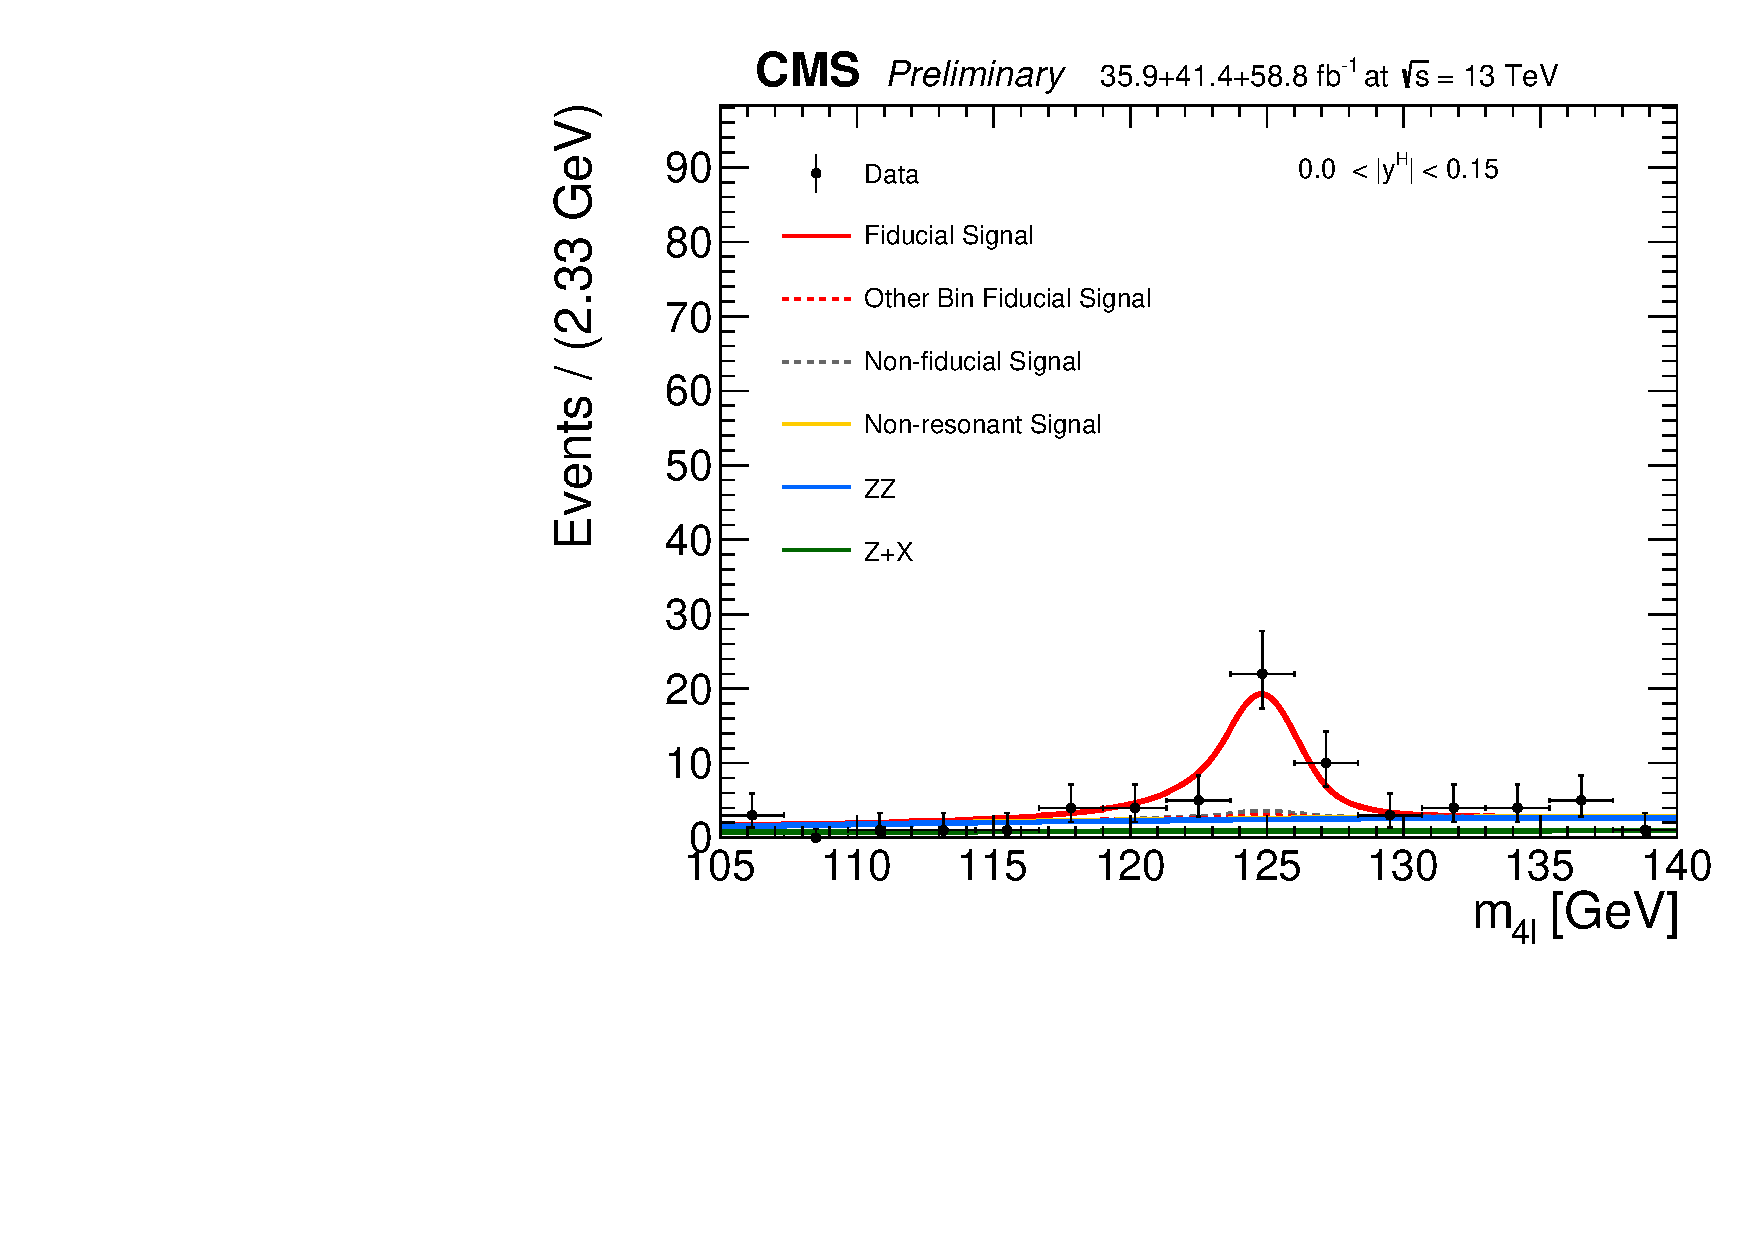
\includegraphics[width=0.32\linewidth]{Figures/results/fiducial/comb/unblind_Feb25/data_unfoldwith_SM_125_v3_rapidity4l_4l_recobin0.pdf}
	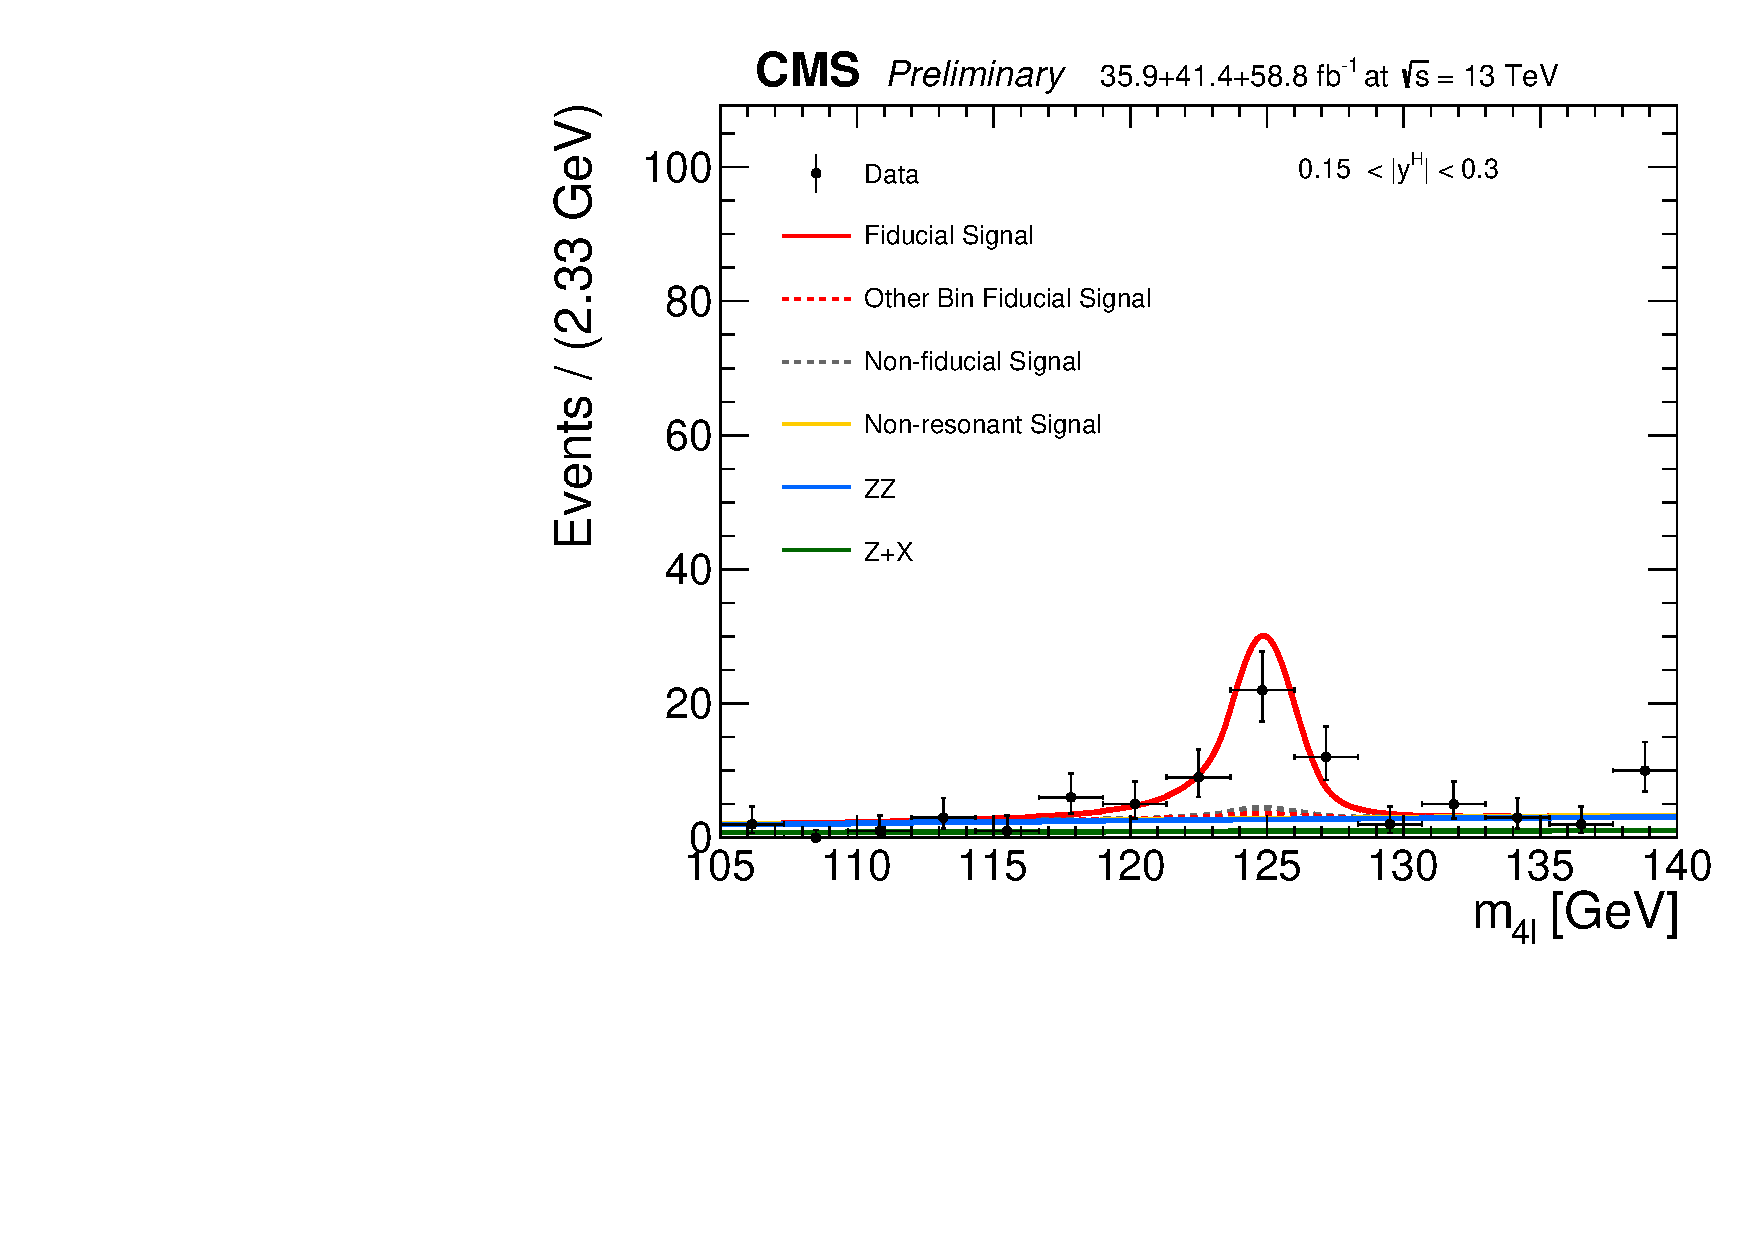
\includegraphics[width=0.32\linewidth]{Figures/results/fiducial/comb/unblind_Feb25/data_unfoldwith_SM_125_v3_rapidity4l_4l_recobin1.pdf}
	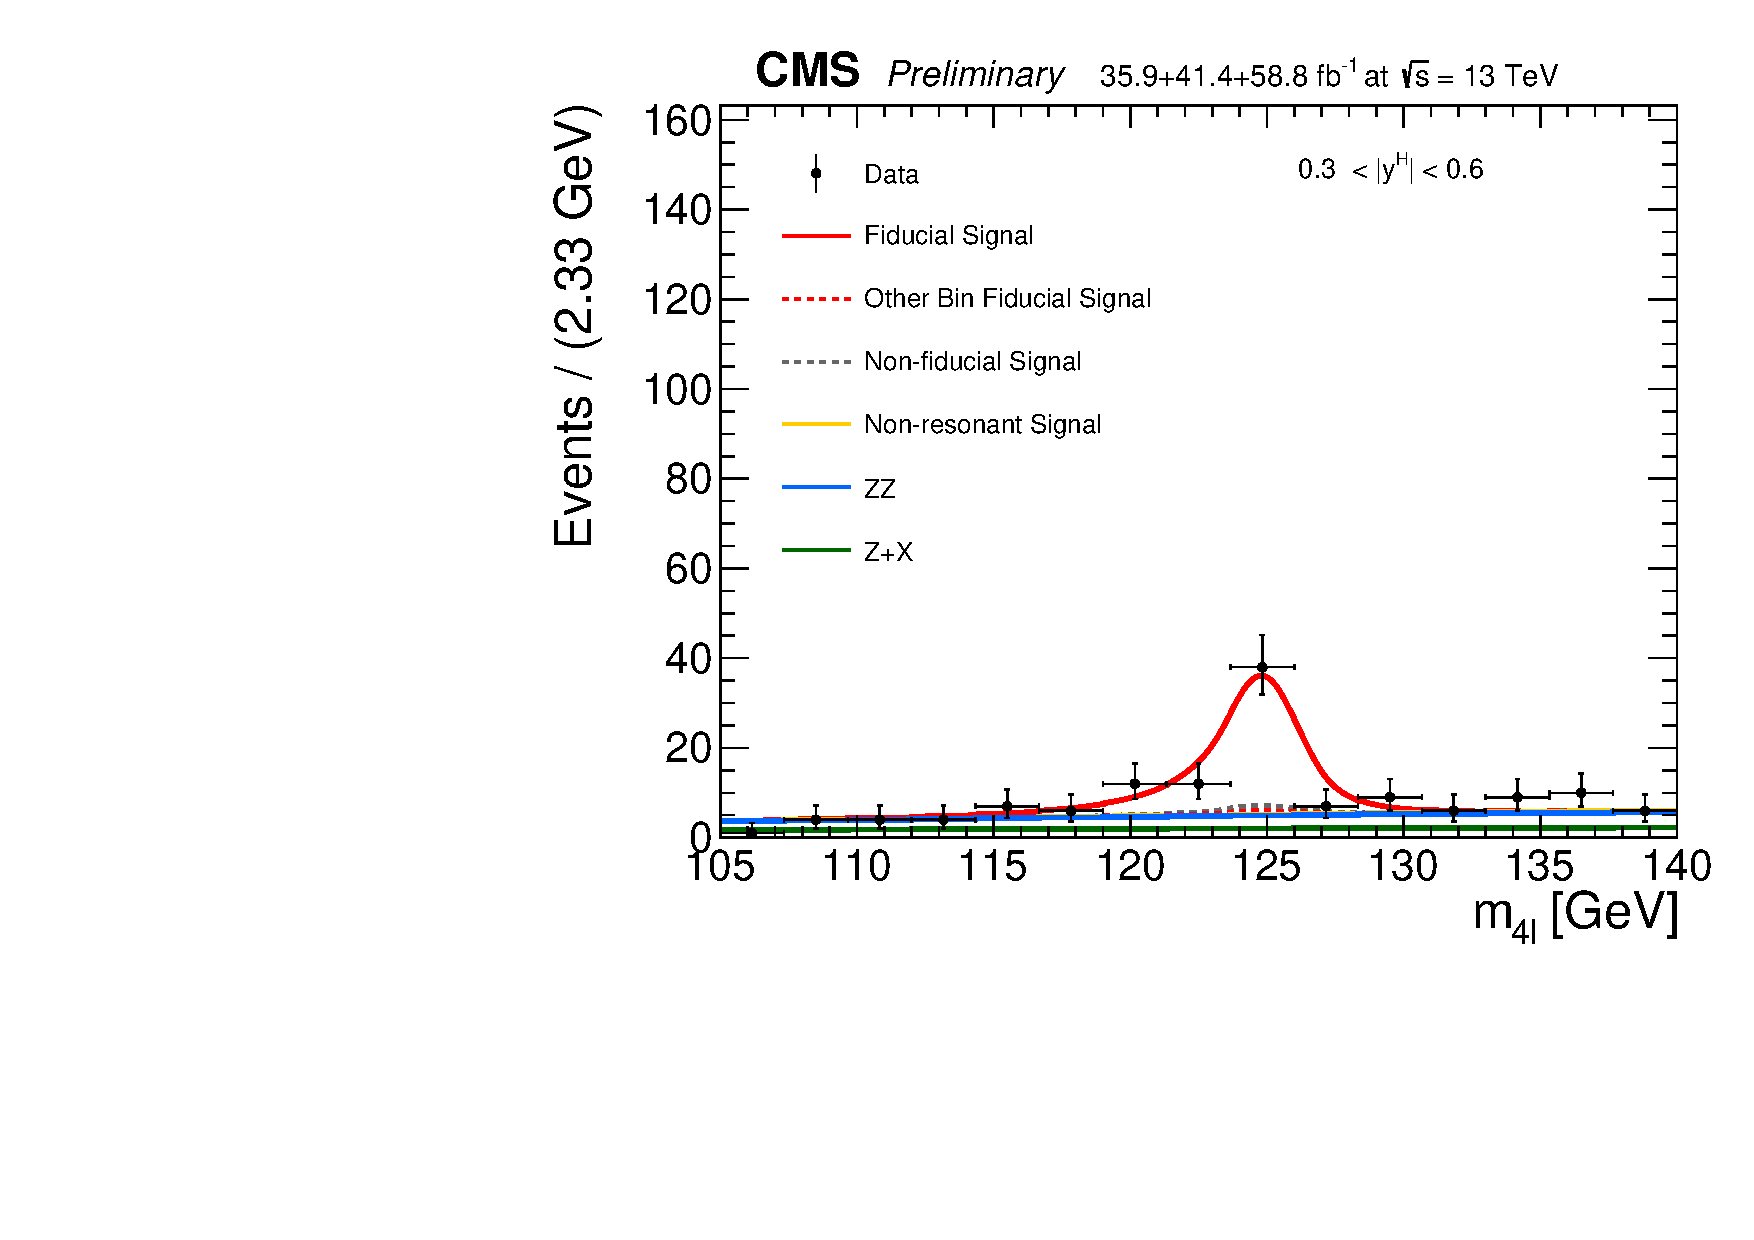
\includegraphics[width=0.32\linewidth]{Figures/results/fiducial/comb/unblind_Feb25/data_unfoldwith_SM_125_v3_rapidity4l_4l_recobin2.pdf} \\
	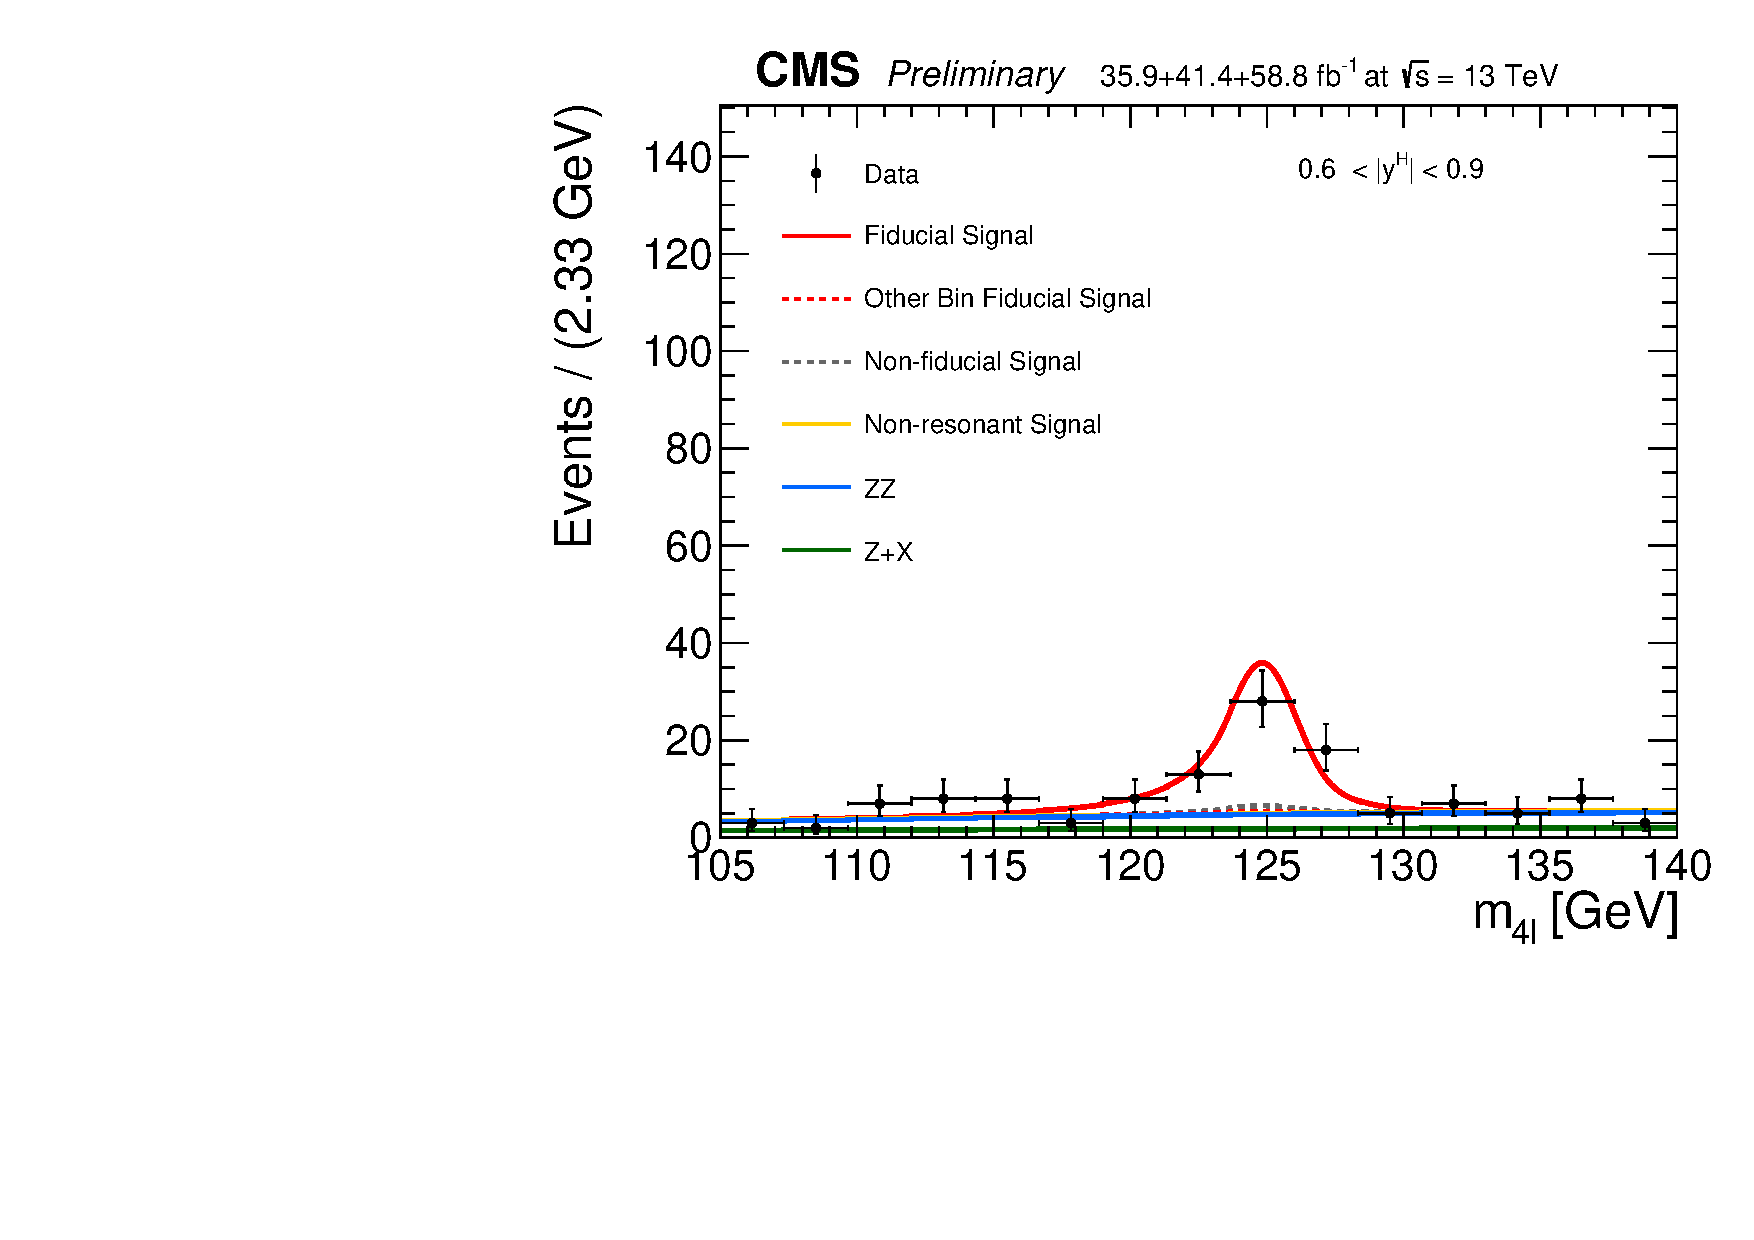
\includegraphics[width=0.32\linewidth]{Figures/results/fiducial/comb/unblind_Feb25/data_unfoldwith_SM_125_v3_rapidity4l_4l_recobin3.pdf}
	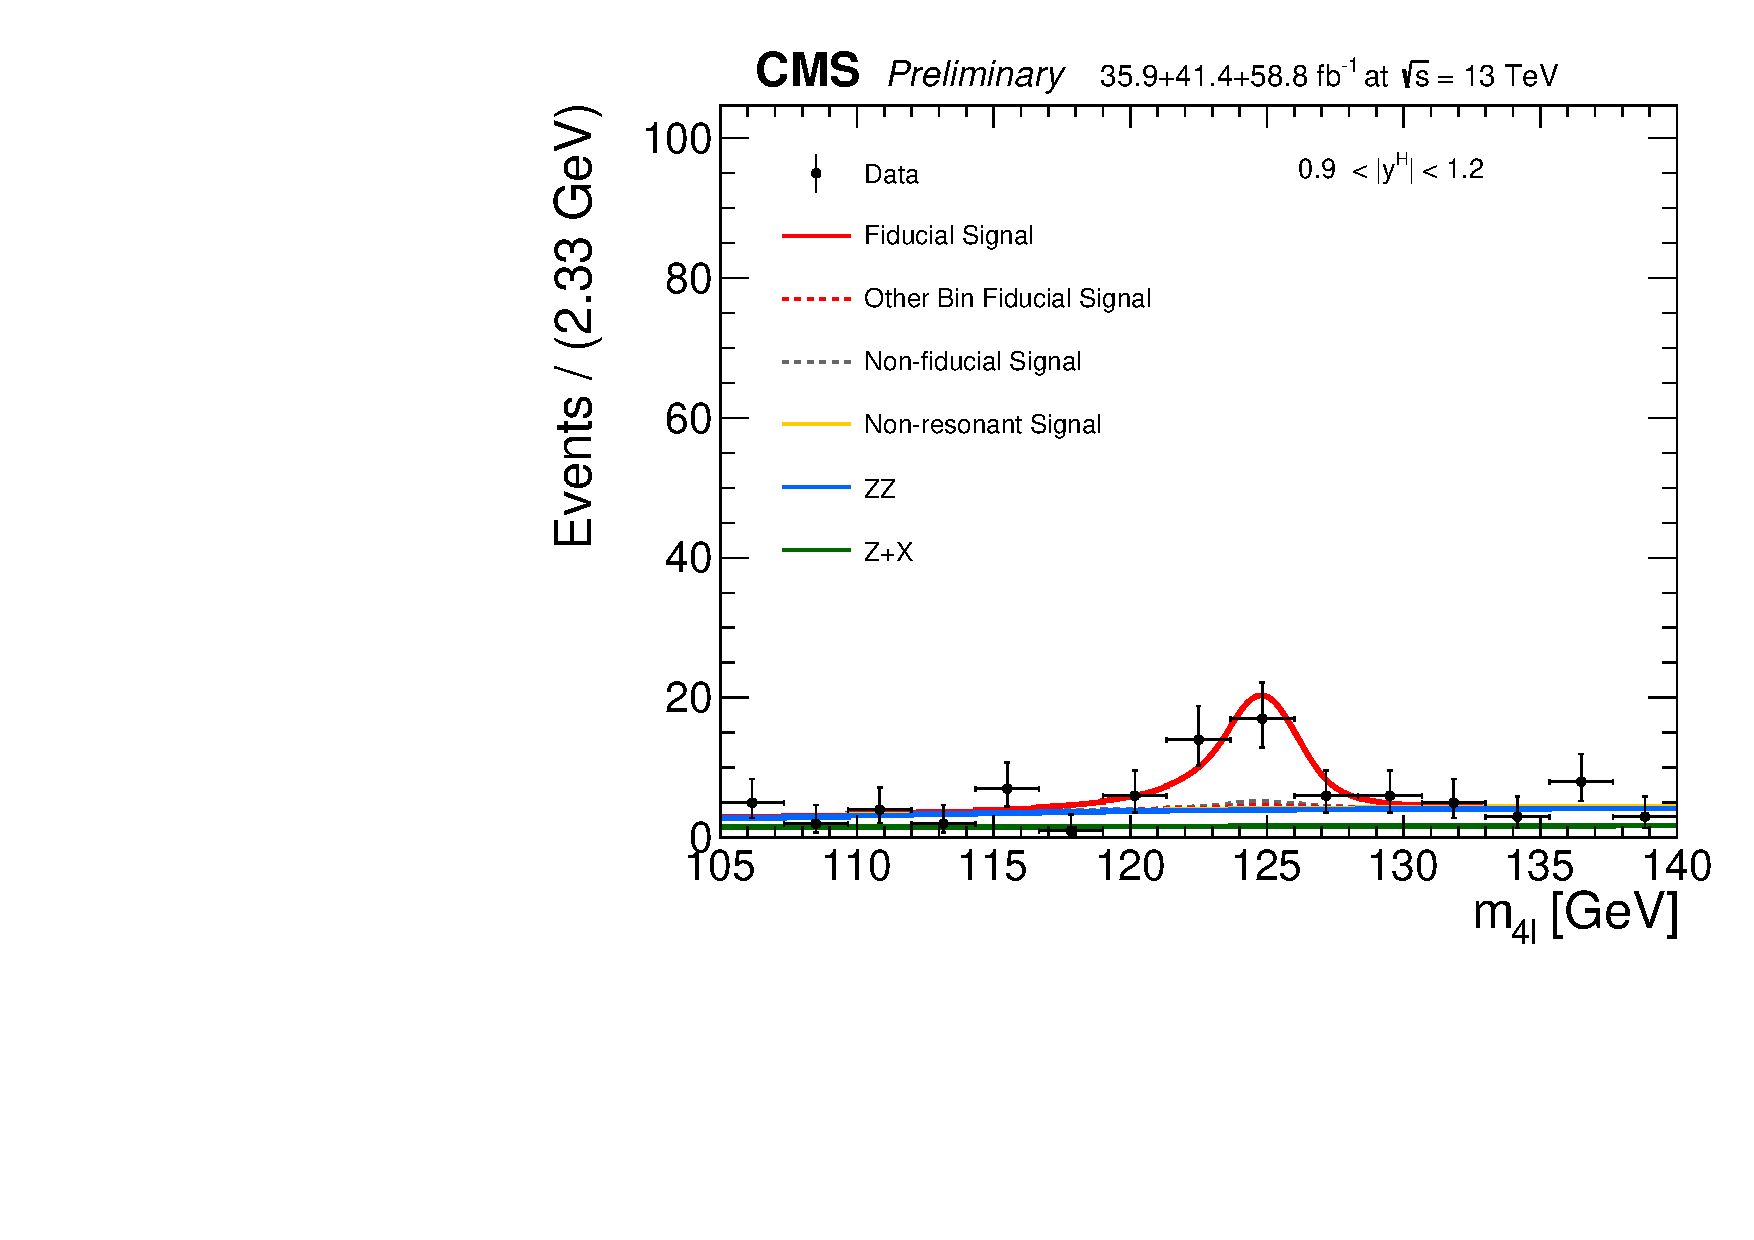
\includegraphics[width=0.32\linewidth]{Figures/results/fiducial/comb/unblind_Feb25/data_unfoldwith_SM_125_v3_rapidity4l_4l_recobin4.pdf}
	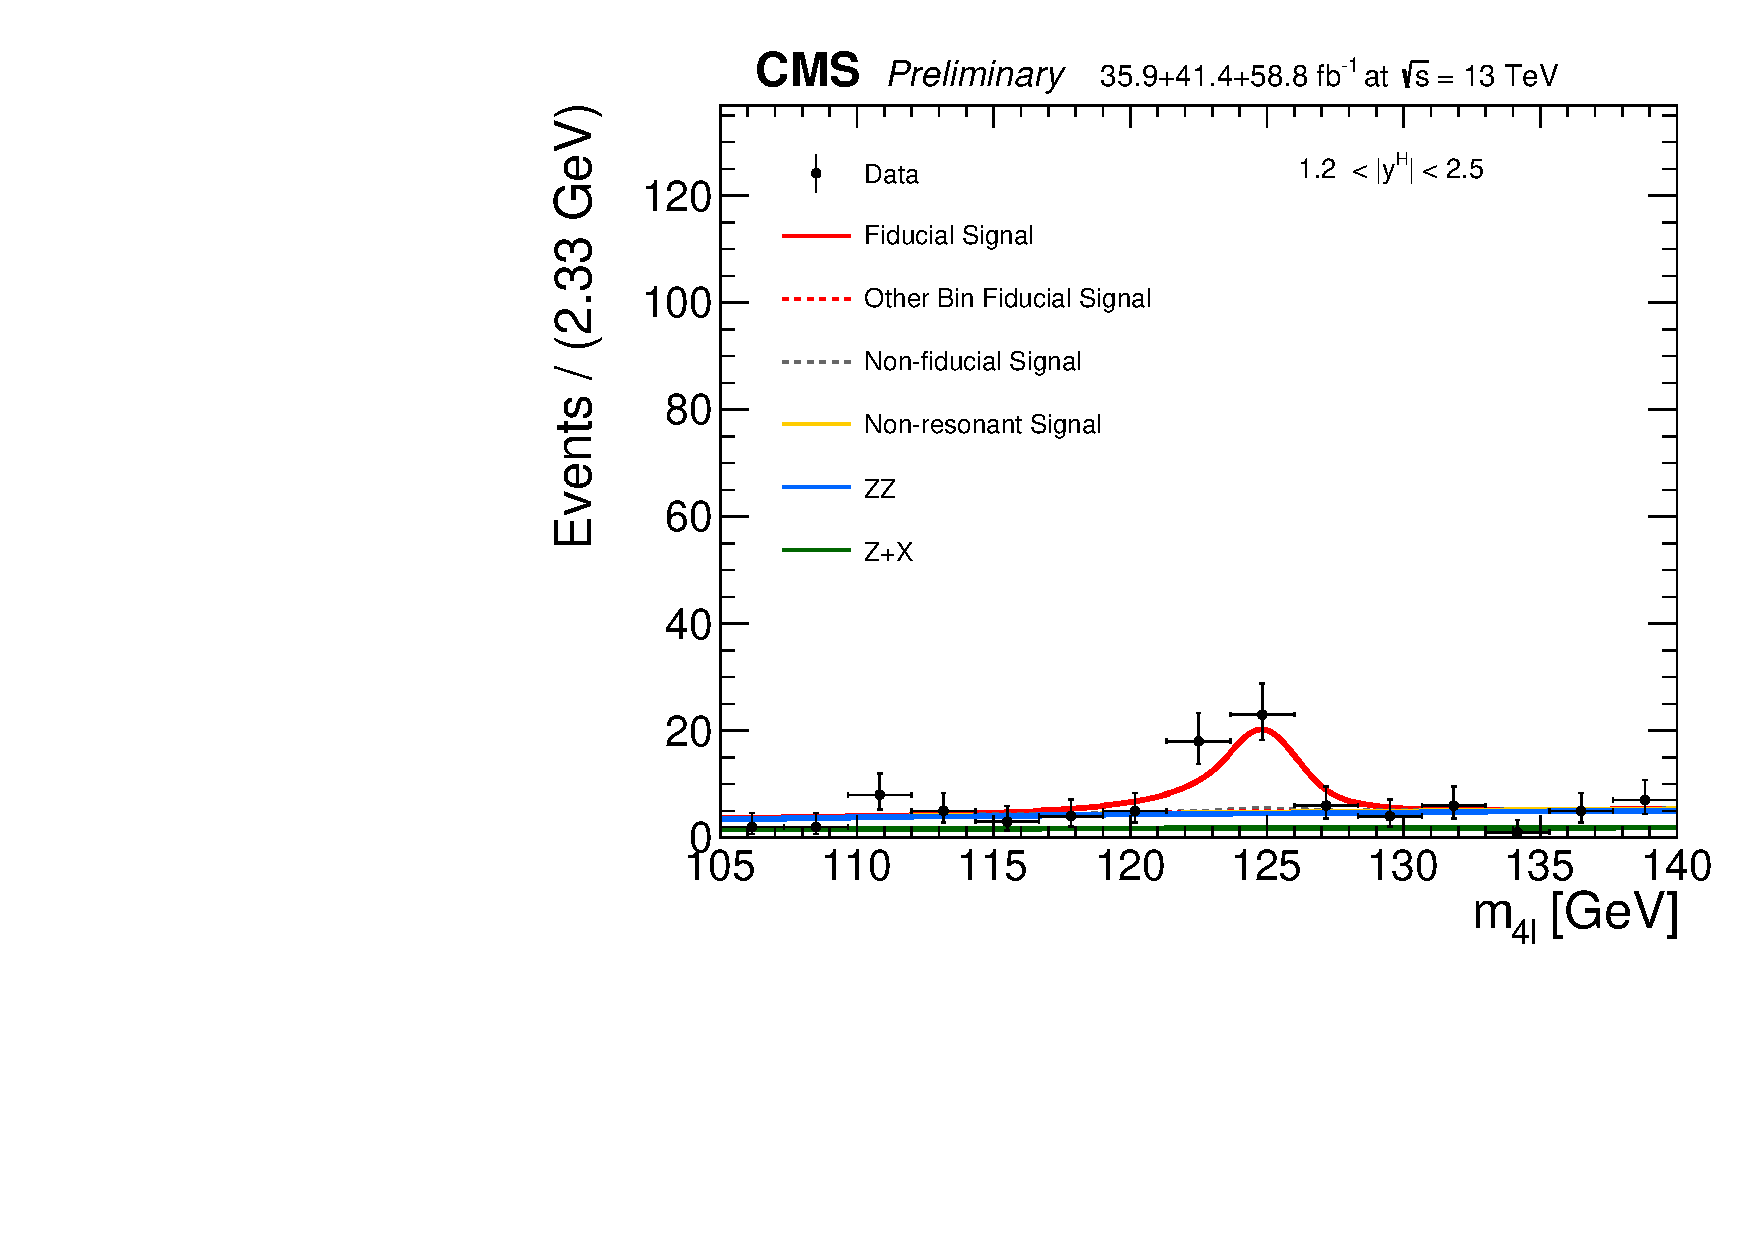
\includegraphics[width=0.32\linewidth]{Figures/results/fiducial/comb/unblind_Feb25/data_unfoldwith_SM_125_v3_rapidity4l_4l_recobin5.pdf}
	\caption{Result of simultaneous fit for the differential fiducial cross section measurement for $y(H)$
		in each differential bin. The combined 4$\ell$ final state is shown. The results are shown for 2018 only. \label{fig:differentialfitNjets}}
\end{figure}


The expected differential cross section results can be seen in Fig.~\ref{fig:fiducialresult}. 

%\begin{figure}[!h]
%	\centering
%	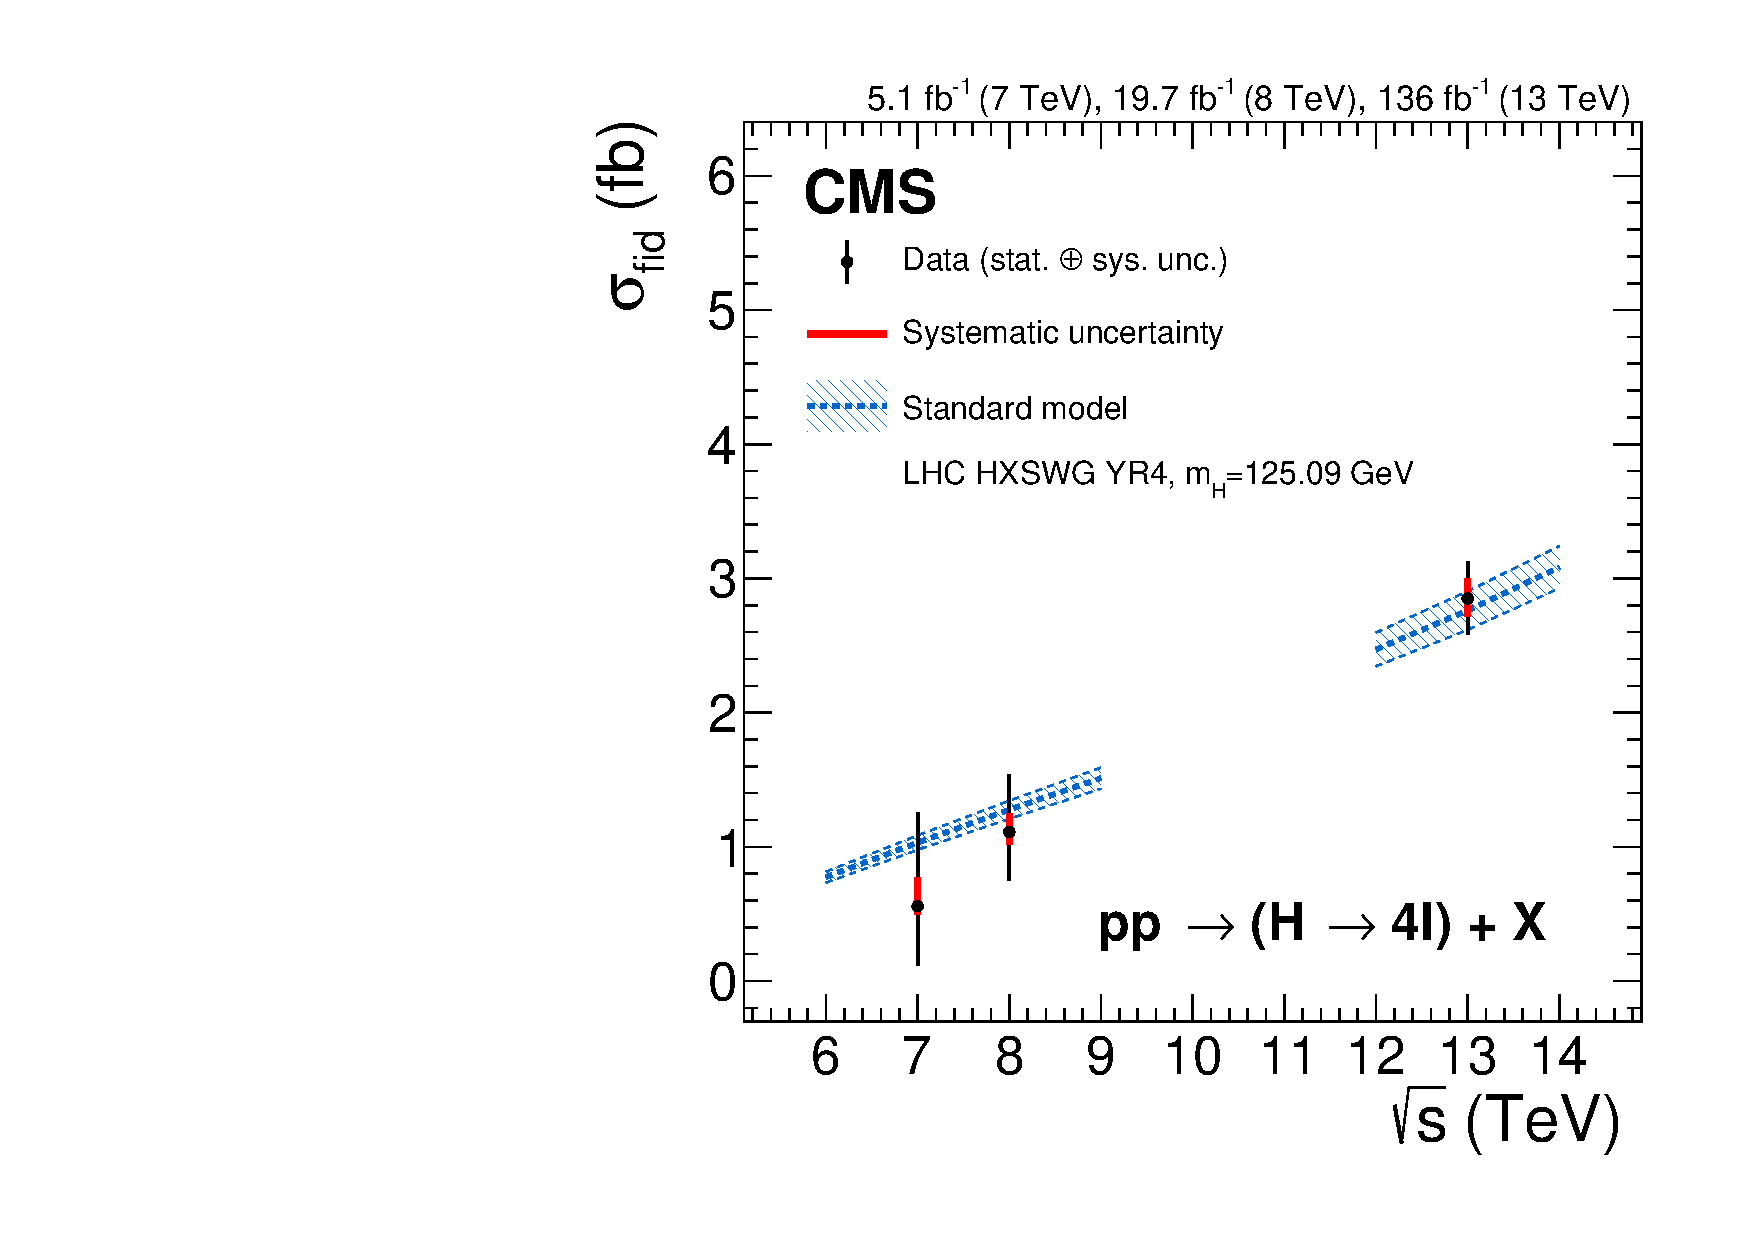
\includegraphics[width=0.45\linewidth]{Figures/results/fiducial/comb/unblind_Feb25/xs_vs_sqrts.pdf}
    % this one is 2016 scaled, to be fixed
%	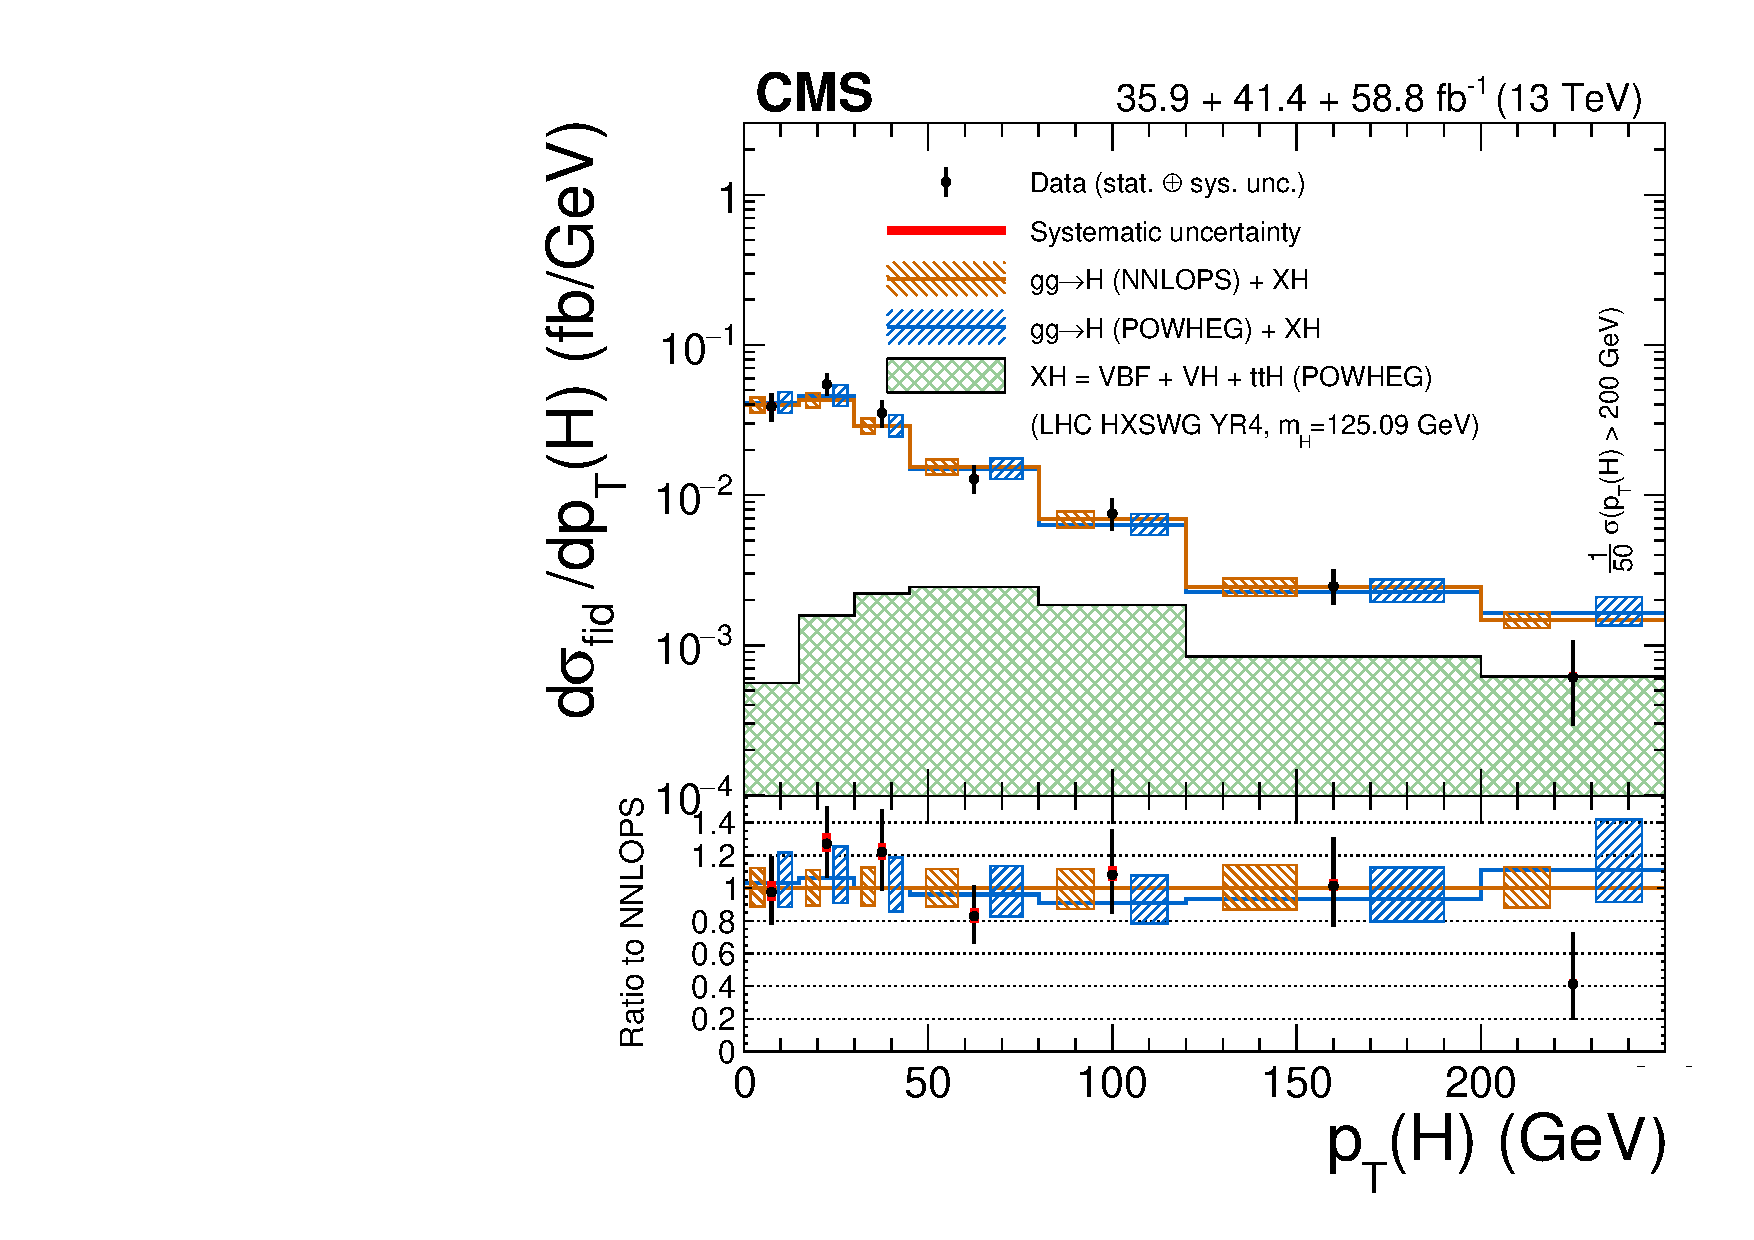
\includegraphics[width=0.45\linewidth]{Figures/results/fiducial/comb/unblind_Feb25/pT4l_unfoldwith_SM_125_logscale.pdf} \\
%	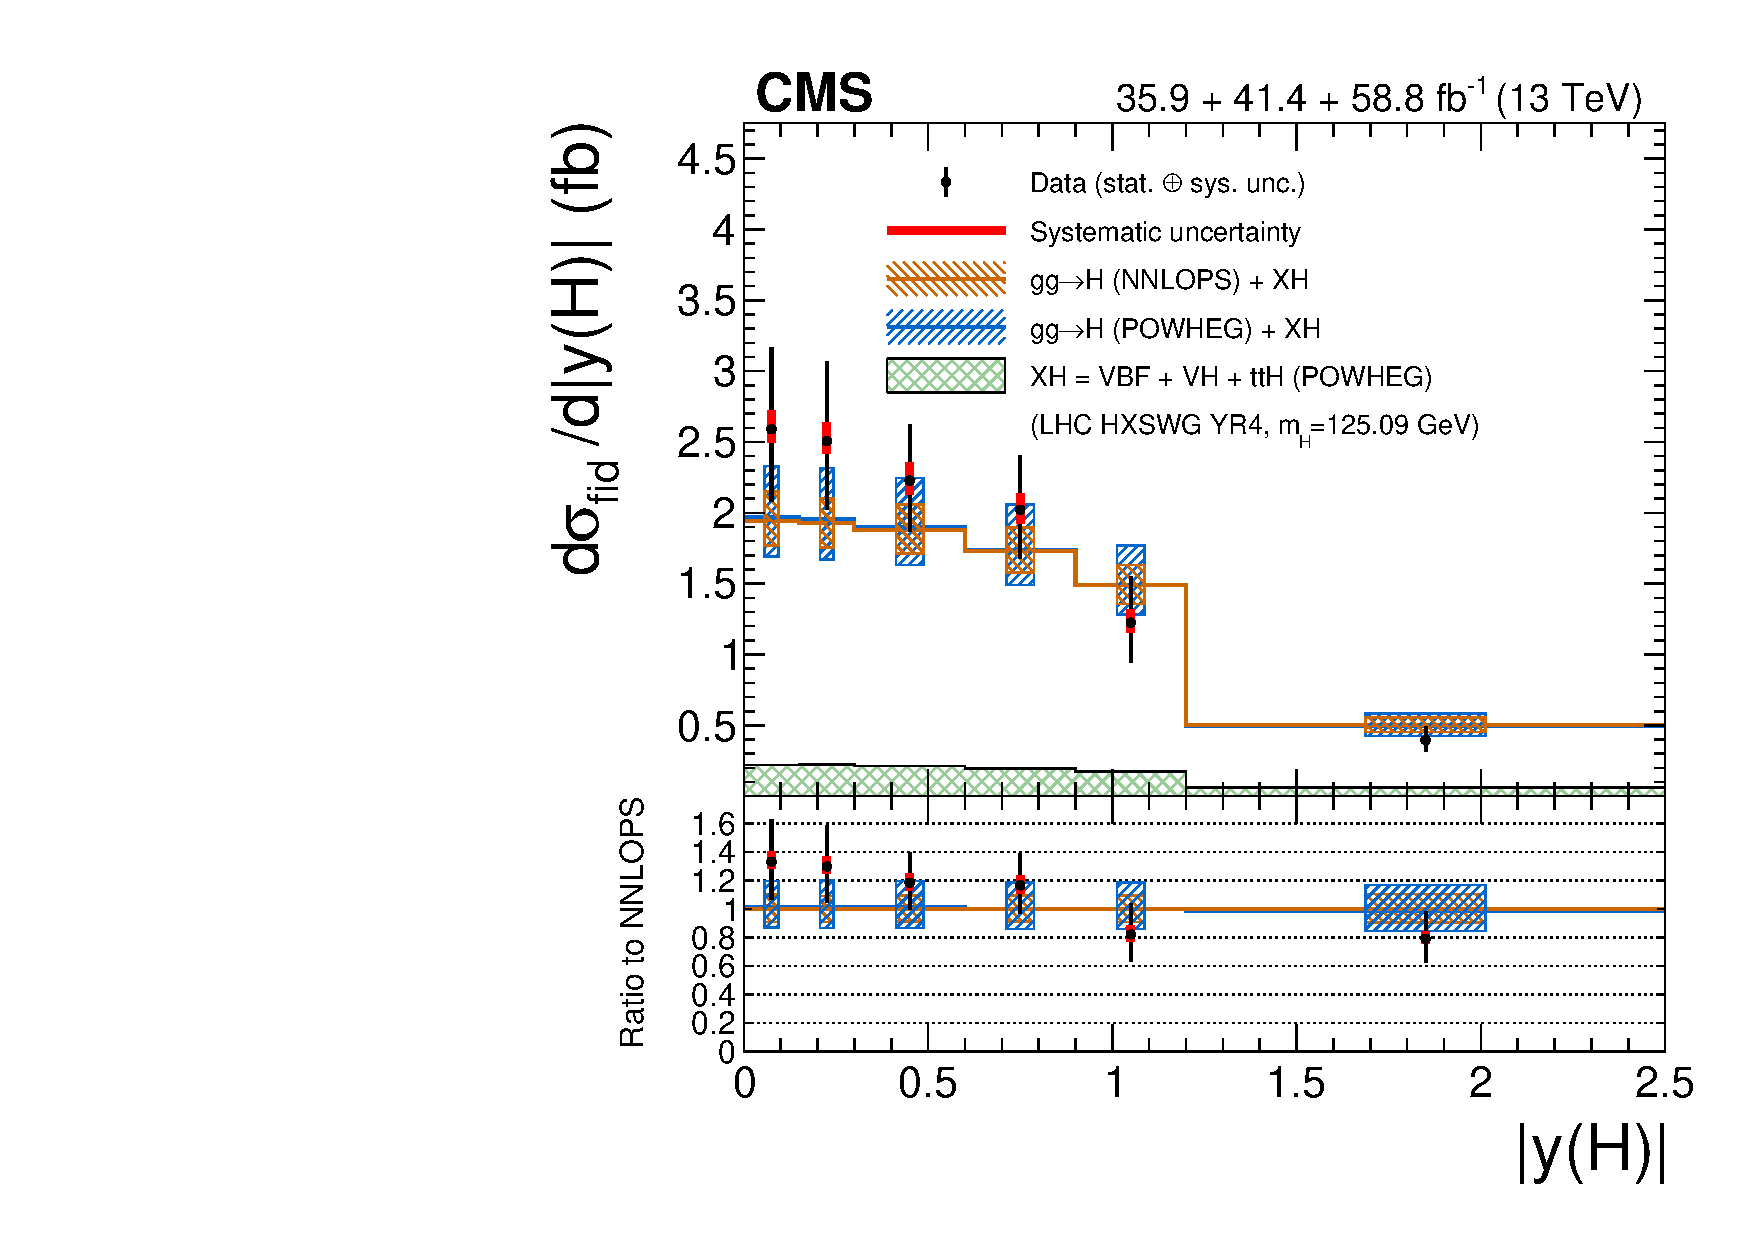
\includegraphics[width=0.45\linewidth]{Figures/results/fiducial/comb/unblind_Feb25/rapidity4l_unfoldwith_SM_125.pdf}
%	\includegraphics[width=0.45\linewidth]{Figures/results/fiducial/comb/scaled_2018/njets_pt30_eta2p5_unfoldwith_SM_125_logscale_asimov.pdf}
%	\caption{Result of the integrated fiducial cross section and the differential cross section measurements for $\pt({\rm H})$, $y({\rm H}$, and N(jets). {\color{red} Lepton scale factors are uncorrelated across years. N(jets) still asimov.} \label{fig:differentialresult}}
%\end{figure}

\begin{figure}[!htb]
        \centering
        \includegraphics[width=0.45\linewidth]{Figures/results/fiducial/comb/mass4l_unfoldwith_SM_125.pdf}
        \includegraphics[width=0.45\linewidth]{Figures/results/fiducial/comb/xs_vs_sqrts.pdf} \\
        \includegraphics[width=0.45\linewidth]{Figures/results/fiducial/comb/pT4l_unfoldwith_SM_125_logscale.pdf}
        \includegraphics[width=0.45\linewidth]{Figures/results/fiducial/comb/rapidity4l_unfoldwith_SM_125_logscale.pdf} \\
        \includegraphics[width=0.45\linewidth]{Figures/results/fiducial/comb/njets_pt30_eta2p5_unfoldwith_SM_125_logscale.pdf}
        \includegraphics[width=0.45\linewidth]{Figures/results/fiducial/comb/pt_leadingjet_pt30_eta2p5_unfoldwith_SM_125_logscale.pdf}
        \caption{
            The measured inclusive fiducial cross section in different final states (top left). The measured fiducial cross section as a function of $\sqrt{s}$ (top right).  
                The acceptance is calculated using \POWHEG at  $\sqrt{s}$=13\TeV and {\sc HRes}~\cite{Grazzini:2013mca,deFlorian:2012mx} 
                at  $\sqrt{s}$=7 and 8\TeV and the total gluon fusion cross section and uncertainty are taken from 
                Ref.~\cite{Anastasiou2016}. The fiducial volume for $\sqrt{s}$=6--9\TeV uses the lepton isolation definition from 
                Ref.~\cite{CMSH4lFiducial8TeV}, while for $\sqrt{s}$=12--14\TeV the definition described in the text is used.
                The results of the differential cross section measurement for $\pt({\rm H})$ (middle left), $|y({\rm H})|$ (middle right) and N(jets) (bottom left), $p_T$ of the leading jet (bottom right). The acceptance and theoreti
cal uncertainties in the differential bins are are calculated using \POWHEG. 
                The sub-dominant component of the the signal (VBF $+$ VH $+~\ttH$) is denoted as XH. 
                \label{fig:fiducialresult}}
\end{figure}



 
